%% ------------------------------------------------------------------------- %%
\chapter{Results and Discussion}
\label{cap:results}

All the statistical tests shown in the last chapter were applied to all experimental scenarios and then filtered by their significance. In very few scenarios of the study it was possible to conclude that the residuals followed a normal distribution according to Shapiro-Wilk test. Even though in these specific instances the typical ANOVA test could be used (given they're also homoscedastic), it was decided to use only the Kruskal–Wallis test so every experimental scenario uses the same statistical framework.

%% ------------------------------------------------------------------------- %%
\section{Statistical Significance}
\label{sec:stats-significance}

Scenarios with a $p$-value above the 0.05 significance level in the Levene test means it failed to reject the hypothesis that the group variances are different: in practice, the homoscedasticity assumption is considered to be true in these cases. In the Kruskal–Wallis test if the $p$-value is less than the $0.05$ the null hypothesis of equal treatment means is rejected, i.e. in practice it is considered at least one treatment mean is different from the other. When an experimental scenario has enough samples (i.e. it won't return NaN), passed the homoscedasticity assumption and reject the equality of treatment means in the Kruskal–Wallis test it is indicated here as \ok. If either the homoscedasticity test failed or Kruskal–Wallis failed to reject the hypothesis of equal means, it is indicated as \notok. All the results of statistical significance of treatment means are summarized in Table \ref{table:stats-sig}.

An important note about homoscedasticity in these results is that the results can be analyzed even though failing the homoscedasticity assumption. For instance, the treatment means can be individually analyzed taking into the context the experimental scenario it belongs to, and insights can be obtained from it. Even though in this case the Kruskal–Wallis cannot be used, observed behaviors which do not require directly statistical significance are reported if deemed insightful.

\begin{table}[H]
    \centering
    \begin{tabular}{||c|lccccccc||}
        \toprule
                    & &  $\eta_{NE}$ & $\eta_{MD}$ & $\eta_{LR}$ & $\eta_{MD,LR}$ & $\eta_{MD, NE}$  & $\eta_{LR,NE}$ & $\eta_{NE, MD, LR}$\\
        \textbf{Cluster} & \textbf{Metric} & & & & & & & \\
        \midrule
        \multirow{3}{4em}{\Large\centering 1} & $\delta_{AUC}$ & \notok & \notok & \ok & \ok & \notok & \notok & \ok \\
                                            & $\delta_{Brier}$ & \notok & \ok & \notok & \ok & \notok & \ok & \ok \\
                                            & $\delta_{Logloss}$ & \ok  & \ok & \notok & \notok & \ok & \ok & \ok \\
        \midrule
        \multirow{3}{4em}{\Large\centering 2} & $\delta_{AUC}$ & \notok & \ok & \notok & \ok & \notok & \ok & \ok \\
                                            & $\delta_{Brier}$ & \notok & \ok & \notok & \ok & \notok & \ok & \ok \\
                                            & $\delta_{Logloss}$ & \ok  & \ok & \notok & \ok & \ok & \ok & \ok \\
        \midrule
        \multirow{3}{4em}{\Large\centering 3} & $\delta_{AUC}$ & \notok & \notok & \ok & \ok & \notok & \notok & \notok\\
                                            & $\delta_{Brier}$ & \notok & \notok & \notok & \ok & \notok & \notok & \notok \\
                                            & $\delta_{Logloss}$ & \notok & \notok & \notok & \notok & \notok & \notok & \notok\\
        \midrule
        \multirow{3}{4em}{\Large\centering 4} & $\delta_{AUC}$ & \notok & \notok & \notok & \notok & \notok & \notok & \notok\\
                                            & $\delta_{Brier}$ & \notok & \notok & \notok & \ok & \notok & \ok & \ok \\
                                            & $\delta_{Logloss}$ & \notok & \notok & \notok & \ok & \notok & \ok & \ok \\
        \midrule
        \multirow{3}{4em}{\Large\centering 5} & $\delta_{AUC}$ & \notok & \notok & \ok & \ok & \notok & \ok & \ok \\
                                            & $\delta_{Brier}$ & \notok & \ok & \ok &  \ok & \notok & \ok  & \ok \\
                                            & $\delta_{Logloss}$ & \notok & \ok & \ok &  \ok & \notok & \ok & \ok \\
        \midrule
        \multirow{3}{4em}{\Large\centering 6} & $\delta_{AUC}$ & \ok & \notok & \notok & \ok & \notok & \notok & \ok \\
                                            & $\delta_{Brier}$ & \notok & \notok & \notok & \ok & \notok & \notok & \notok \\
                                            & $\delta_{Logloss}$ & \notok & \notok & \notok & \ok & \notok & \notok & \notok \\
        \bottomrule
    \end{tabular}
    \caption{All experimental scenarios and their respective Kruskal–Wallis results for equality of treatment means}
    \label{table:stats-sig}
\end{table}

Some interesting insights can be made by inspecting the statistical significance results in Table \ref{table:stats-sig} and the specific $p$-values for the tests in the Table \ref{Appendix} in the Appendix:

\begin{enumerate}
    \item For instance, Cluster 3 scenarios failed most of the homoscedasticity tests, but by visually analyzing the $\delta_{metric}$ plot it displays the same behavior of the treatments as the other clusters. However, Cluster 3 datasets are all synthetically generated (as illustrated in Table \ref{table:1}), and this can be a reason why it has so few statistically significant results. In Figure \ref{fig:res-failed-c3} one $\delta_{AUC}$ plot from Cluster 3 results is illustrated.
    \begin{figure}[H]
        \centering
        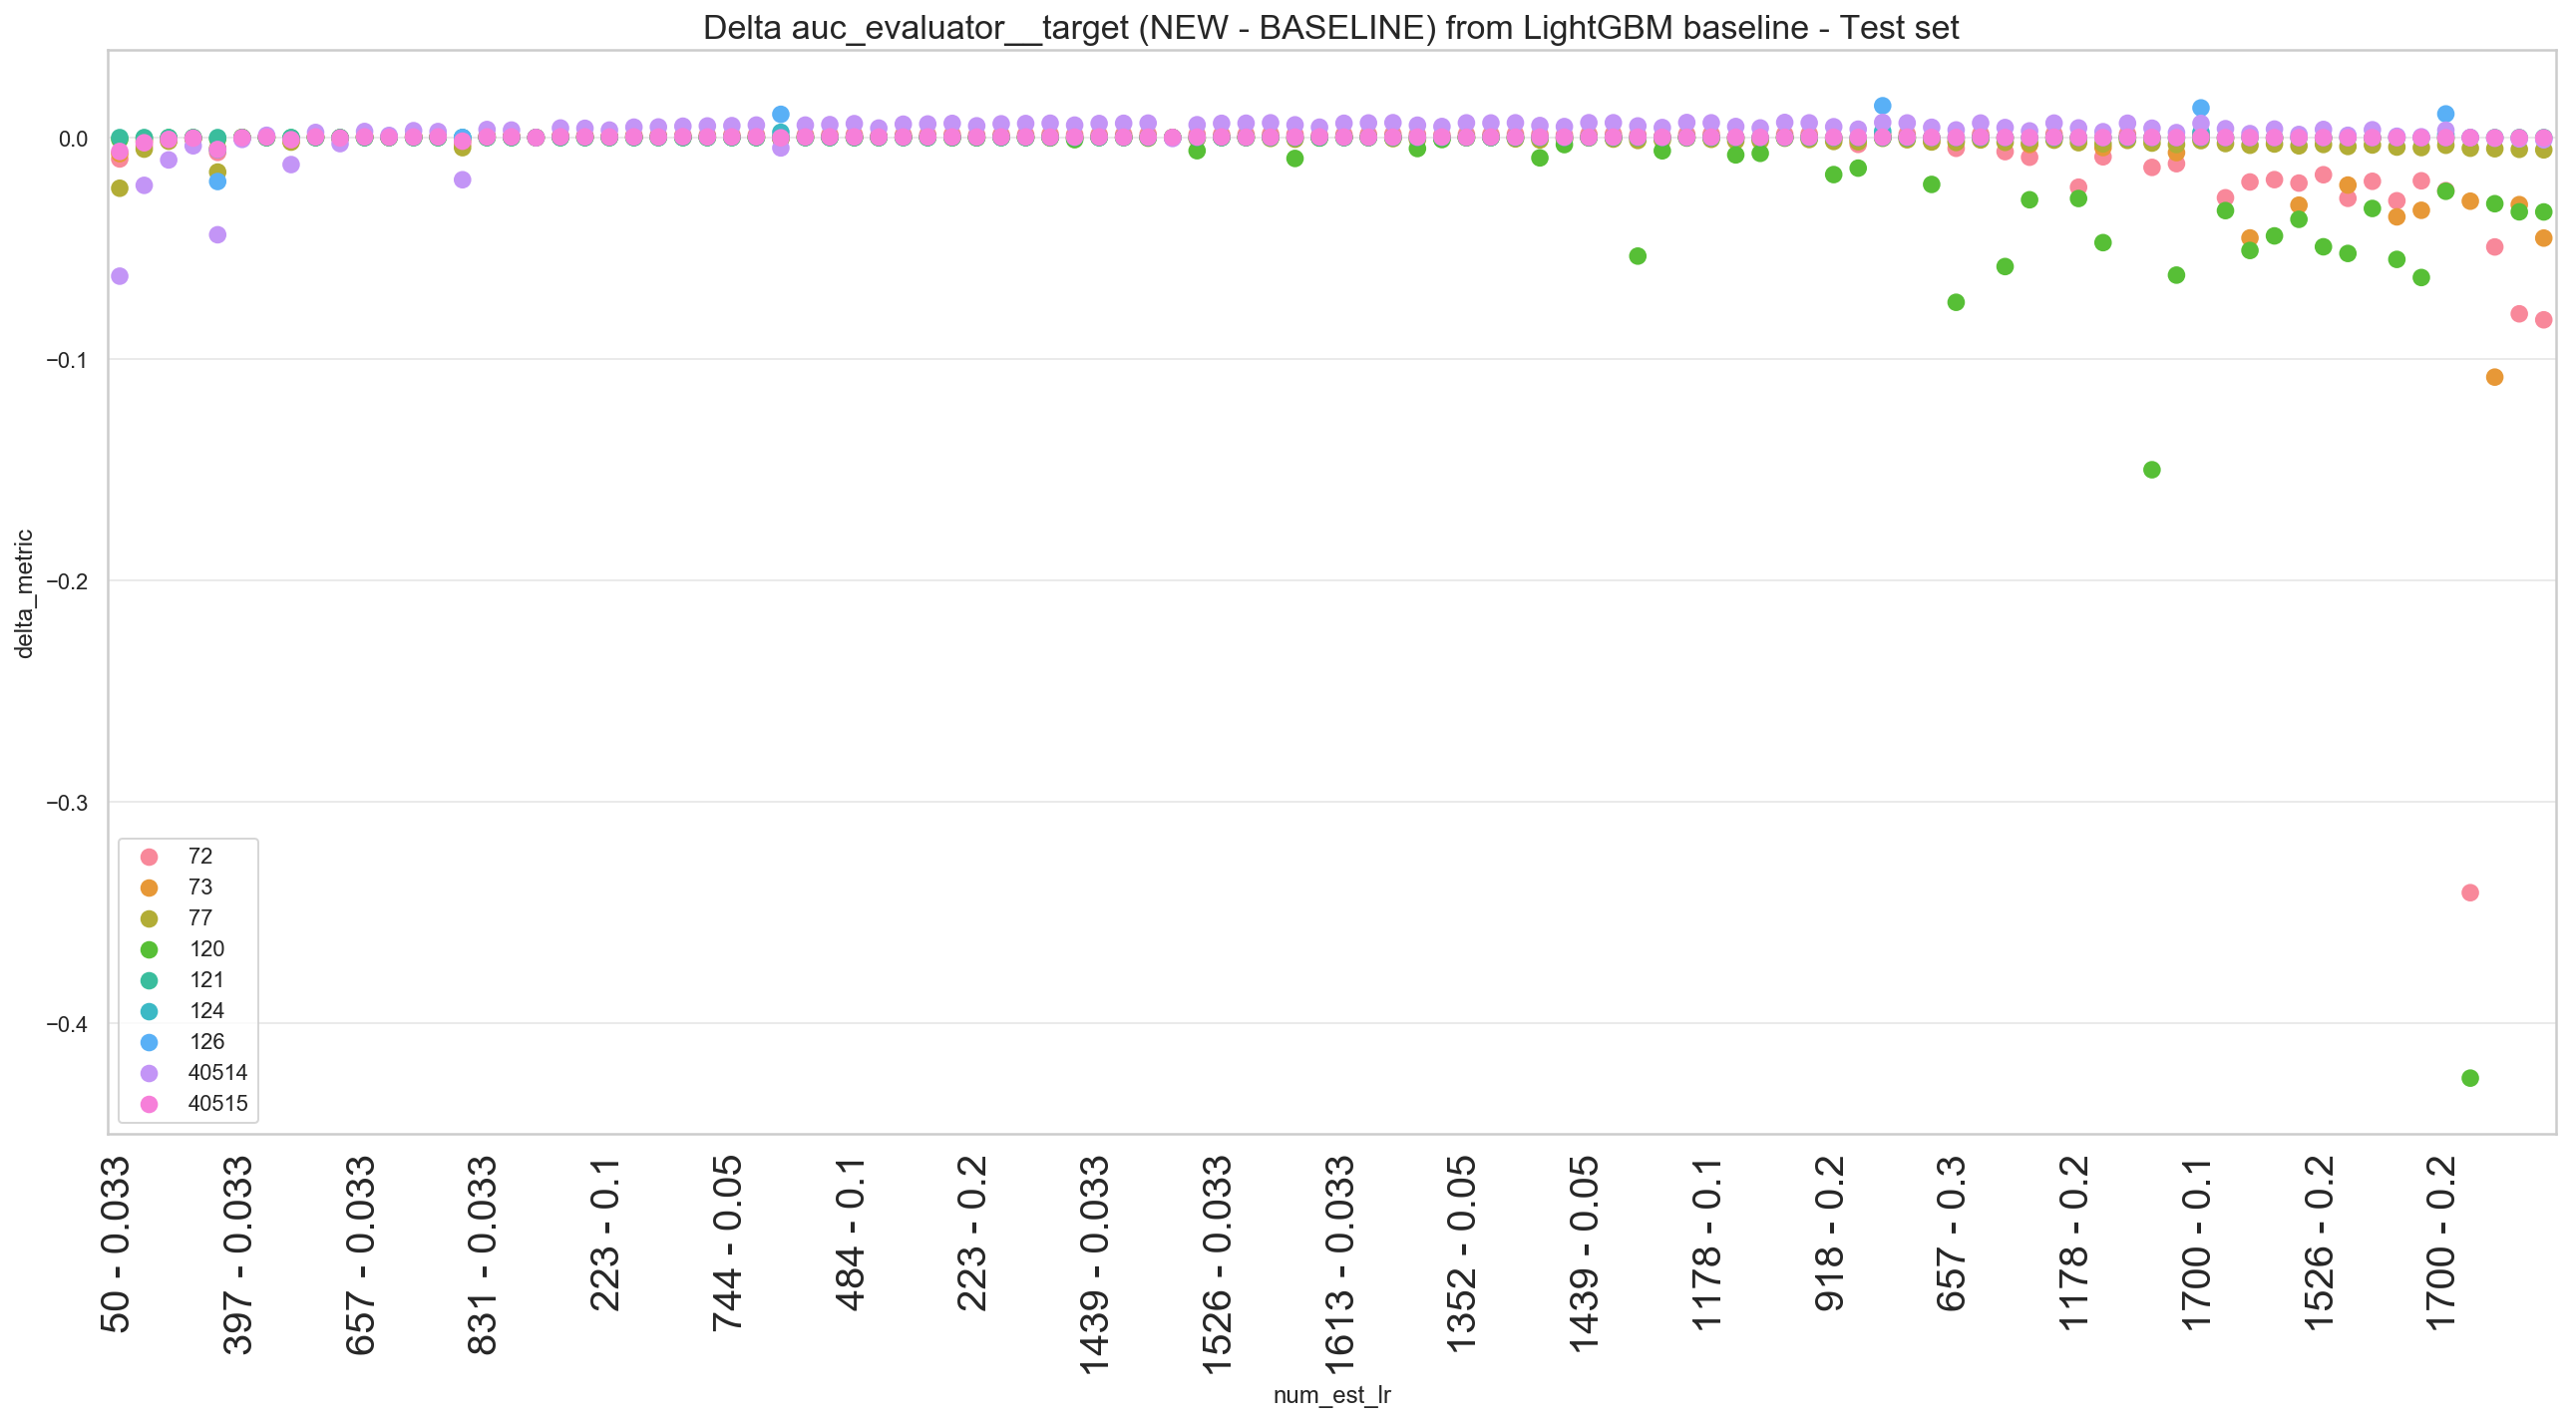
\includegraphics[width=1\textwidth]{delta-auc-cluster3-failed.png} 
        \caption{$\delta_{AUC}$ for scenario $\mathcal{S}(C_3, \eta^{(3)}_{LR, NE}, AUC)$, which failed the Levene Test; Some datasets $\delta_{AUC}$ increased the variance in treatment groups with very high learning rate and number of estimators}
        \label{fig:res-failed-c3}
    \end{figure}
    \item Analyzing Table \ref{table:stats-sig} column-wise, the experiments changing the number of estimators ($\eta_{NE}$) and changing both the number of estimators and maximum depth ($\eta_{MD, NE}$) have very few scenarios where there's a significant change in the performance metrics.
    \item Overall, the Brier Score and Logloss metrics are relatively more sensitive when compared to AUC in the analyzed datasets.
\end{enumerate}

In experimental analysis, if a statistically significant result of a parametric or nonparametric analysis of variance is obtained on the experimental data, a \textit{post hoc} test is used to assess the difference between group treatments results, as described in \cite{Terpilowski2019}. In this study the results of the post hoc tests are not analyzed here, although it could be useful in future work. For this reason, the analysis pipeline implemented in the code has the option to perform a pair-wise Conover test (using the Holm–Bonferroni method to correct for \textit{family-wise error rate}) on all treatment means. In Figure \ref{fig:posthoc-conover} it is shown one example of a Conover test of the experimental scenario $\mathcal{S}(C_1, \eta^{(1)}_{LR}, Brier)$, to exemplify\footnote{This is just an example plot that wasn't used in the analysis, since the scenario is not statistically significant according to Kruskal–Wallis.}.

\begin{figure}[H]
    \centering
    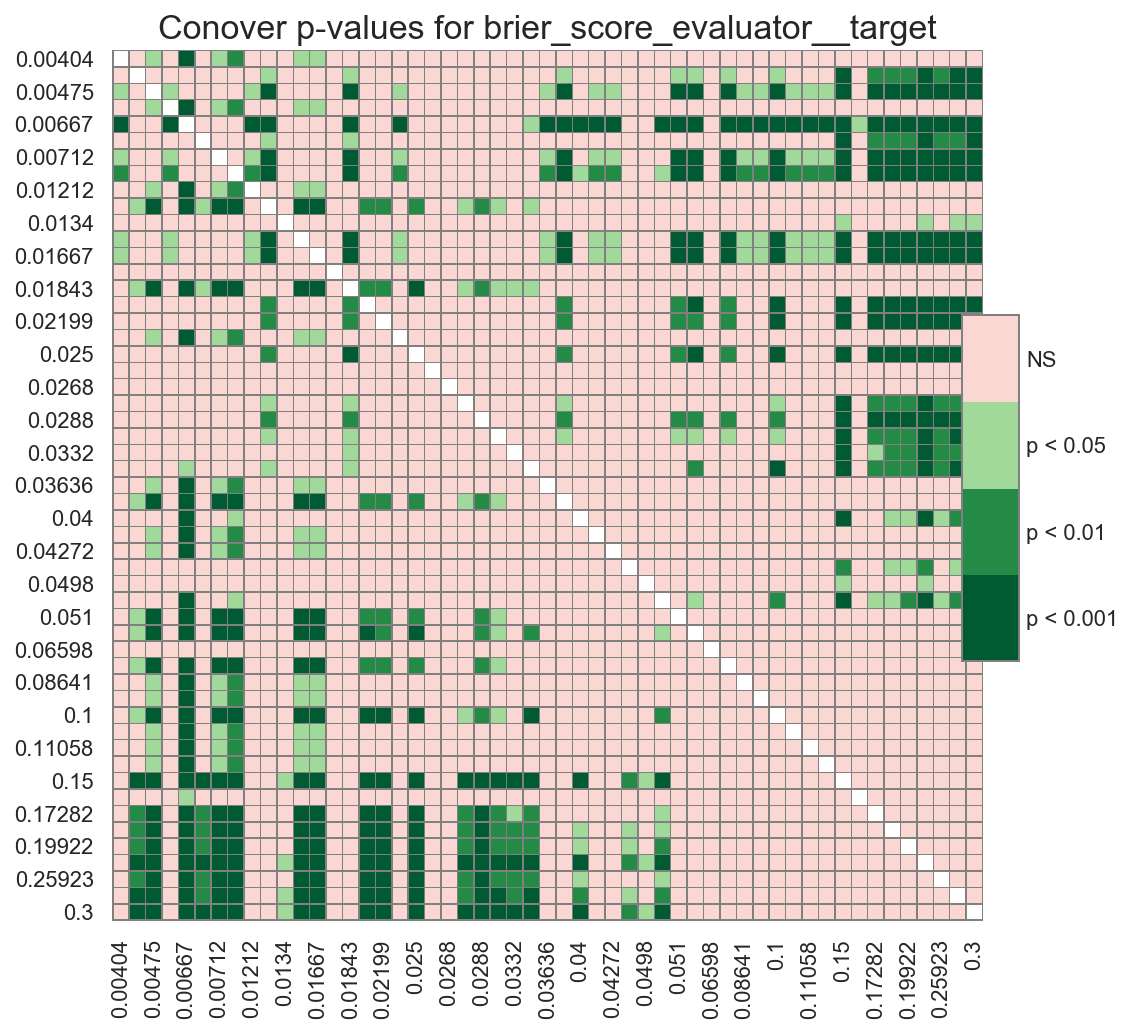
\includegraphics[width=.75\textwidth]{conover-cluster1.png} 
    \caption{Example of post hoc plot with the pairwise differences in treatment means}
    \label{fig:posthoc-conover}
\end{figure}

%% ------------------------------------------------------------------------- %%
\section{Treatment Effect and Single-Factor Plots}

In the analysis, a SFM model is fitted for every experimental scenario. After the statistical testing, the calculated SFM model is then visualized using the \textit{SFM plot}, a very important plot to understand the overall behavior of the estimated treatment effects $\hat{\tau_i}$ w.r.t the overall estimated mean $\hat{\bm{\mu}}$. The defined ordering of the treatment values, defined in Subsection \ref{subsec:ordering} is very useful in this step to grasp the general impact in the metrics of an experimental scenario. To correctly understand the SFM plot, in Figure \ref{fig:sfm-plot-c3-mdlr} the processed SFM plot for scenario $\mathcal{S}(C_3, \eta^{(3)}_{MD, LR}, AUC)$ is illustrated. All SFM plots have two components:

\begin{figure}[H]
    \centering
    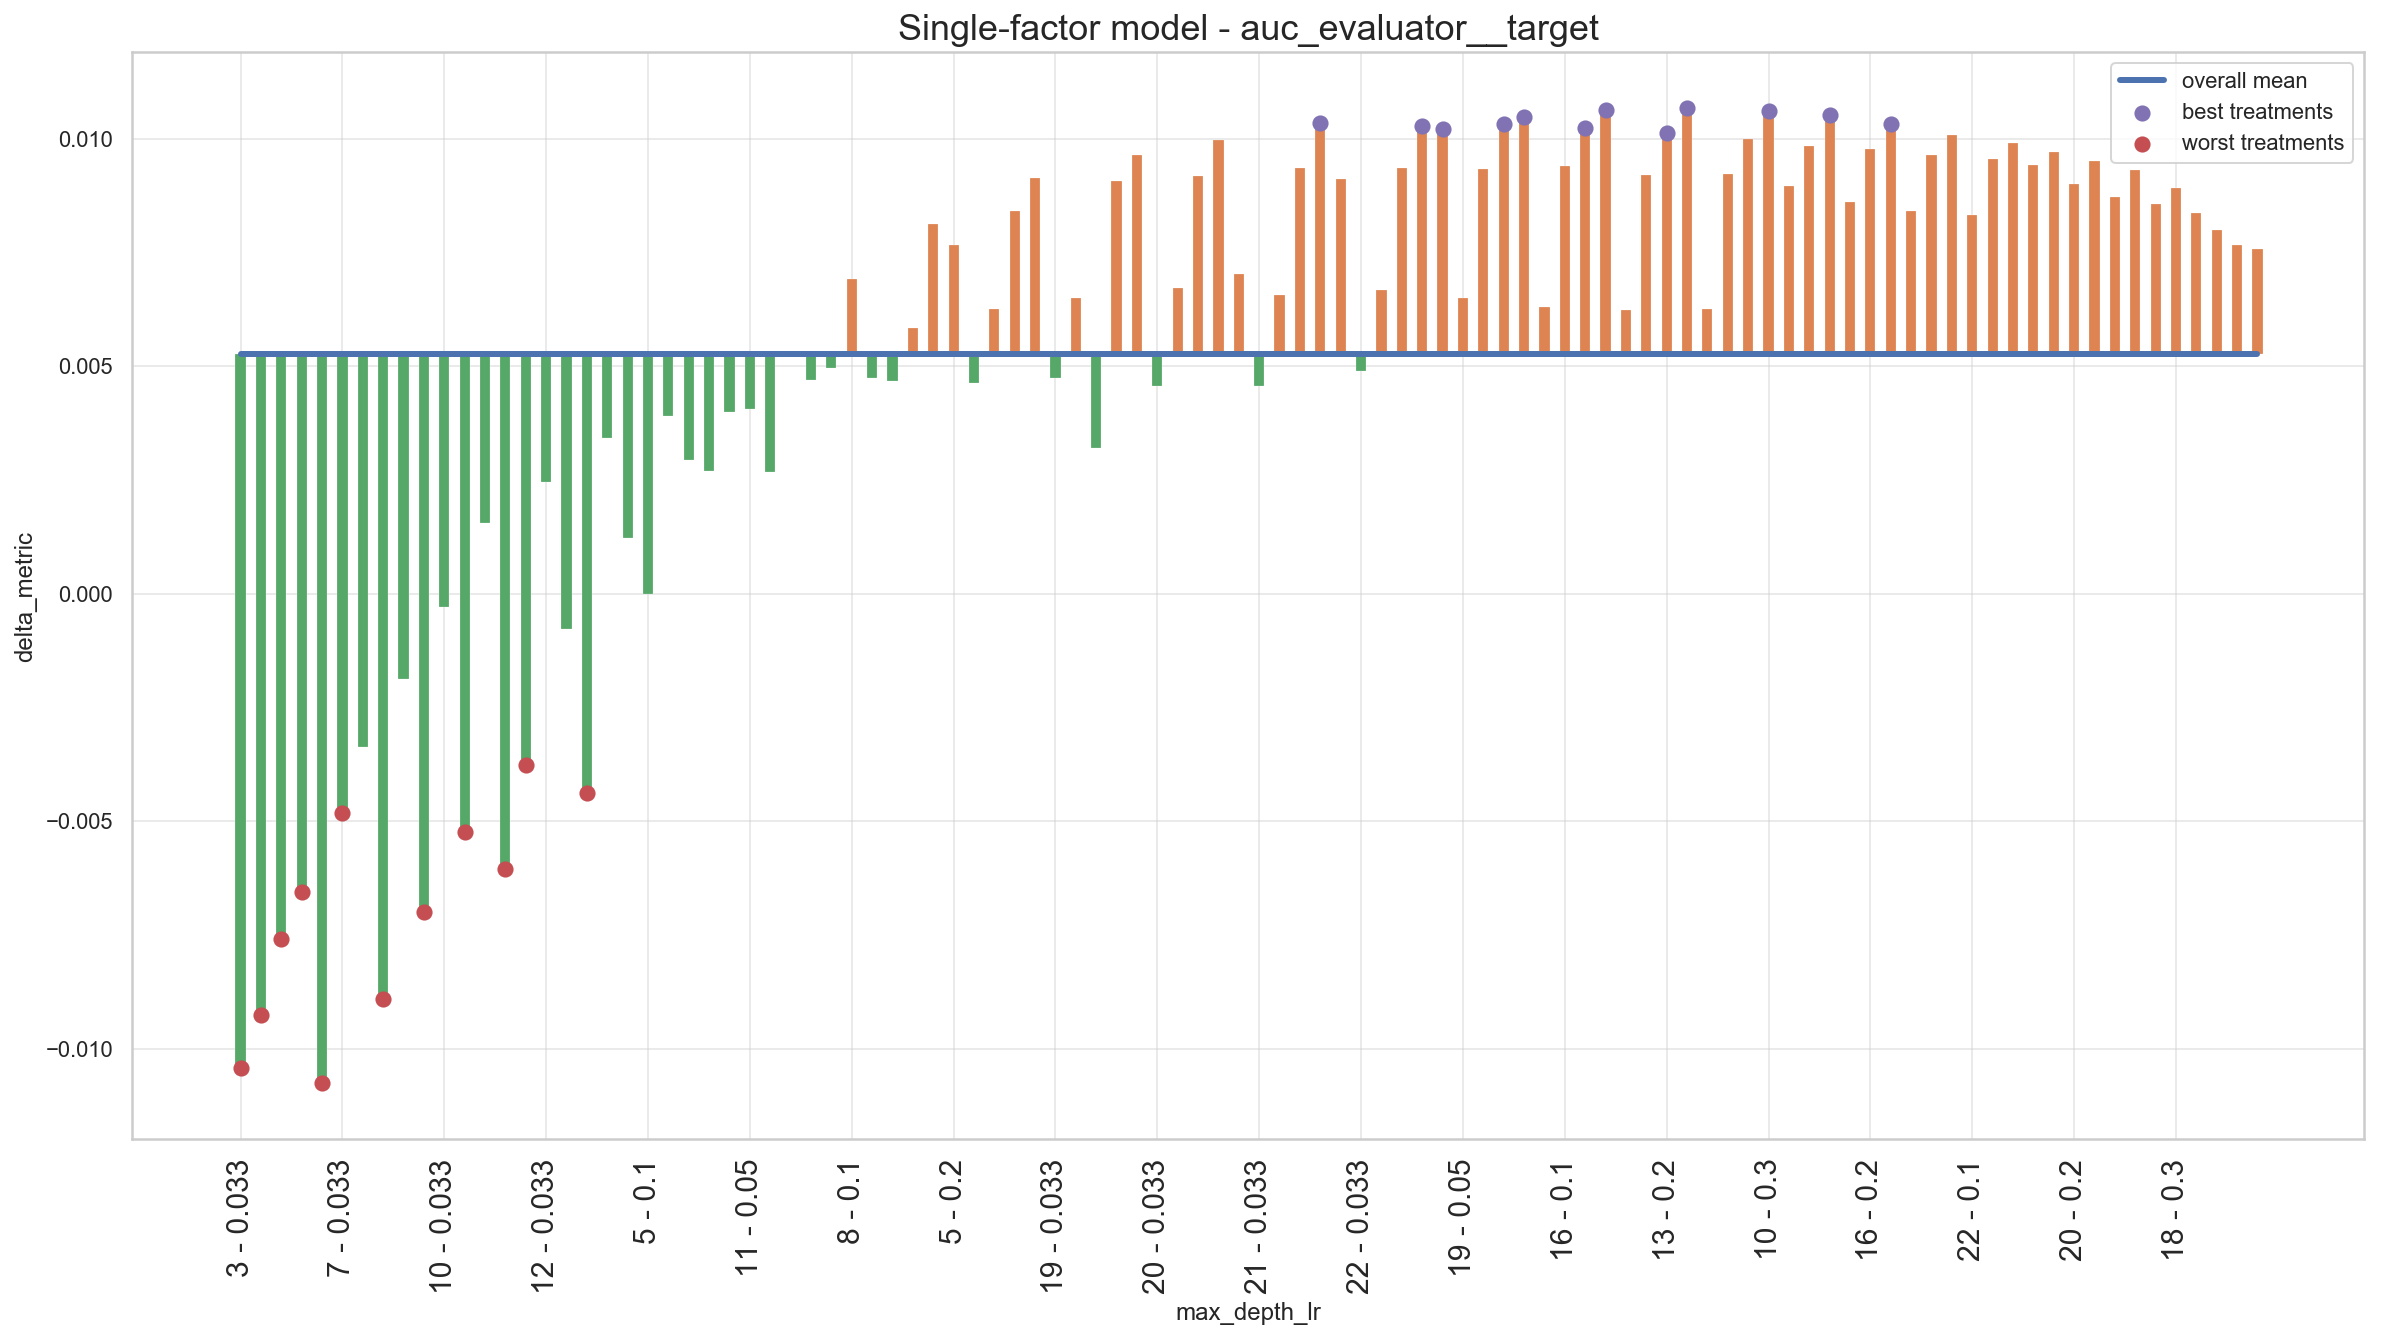
\includegraphics[width=1\textwidth]{sfm-cluster3-mdlr.png} 
    \caption{SFM plot of  $\mathcal{S}(C_3, \eta^{(3)}_{MD, LR}, AUC)$}
    \label{fig:sfm-plot-c3-mdlr}
\end{figure}


\begin{enumerate}
    \item The \textbf{overall mean} is the estimated average effect $\hat{\bm{\mu}}$. In practice, it means what is the average change in the performance metric of the LightGBM classification model of the current cluster when subjected to all treatment values  $\eta^{(k)}_Q$.
    \item The vertical lines in the plot are the estimated treatment effects $\hat{\tau_i}$ of each treatment value (shown in the x axis). The colors \textcolor{orange}{orange} and \textcolor{ForestGreen}{green} distinguish treatments higher and lower than  $\hat{\bm{\mu}}$, respectively.
    \item For each SFM plot, the $\hat{\tau_i}$ with the highest and lowest value are calculated and highlighted in two groups:
    \begin{enumerate}
        \item The \textbf{best treatments} are the treatments that provide the highest improvement on the performance metric. As explained on Subsection \ref{subsec:delta-metrics}, this depends on the metric being chosen: in Figure \ref{fig:sfm-plot-c3-mdlr} a positive $\delta_{AUC}$ means a model with a higher AUC than baseline, so the highest \textcolor{orange}{orange} lines are the best treatments in this case.
        \item The \textbf{worst treatments} are the treatments that have the worst impact on the performance metrics, i.e. treatments that generates models with worse metrics than the baseline. Again, it depends on the metrics being chosen: in the case of AUC the worst treatments are the ones where the $\delta_{AUC}$ is the lowest in absolute value, but for Logloss and Brier Score this interpretation is reversed. In Figure \ref{fig:sfm-plot-c3-mdlr} the worst cases for this specific scenario are low values of both learning rate and maximum depth, i.e. the lowest \textcolor{ForestGreen}{green} lines.
    \end{enumerate}
\end{enumerate}

The SFM plots are the final plots for the analysis done in this study. They become increasingly difficult to read the higher the dimensionality of the treatments, i.e. the higher the number of different hyperparameters being changed at the same time.

%% ------------------------------------------------------------------------- %%
\section{Result by Hyperparameters}

In this part, the hyperparameters combinations are analyzed individually for their impact obtained with the experimental results.

\subsection{\texorpdfstring{\Large$\eta_{NE}$}{}}
\label{subsec:res-ne}

By analyzing the results of the Kruskal–Wallis tests, without considering the homoscedasticity test, the number of estimators is the hyperparameter that have the least impact on the metrics, on all clusters. The proportion of times this hyperparameter actually provided a significant difference for $\delta_{AUC}$, $\delta_{Brier}$ and $\delta_{Logloss}$ were approximately 16\%, 16\% and 50\% respectively. That is, from all the experimental scenarios with treatments of only changing the number of estimators ($\eta_{NE}$), almost none of them had a significant difference in AUC and Brier Score.

When analyzing the SFM plots, a peculiar behavior was observed on the results of $\eta_{NE}$ experiments. The treatments effects are very noisy, with many intercalating positive and negative results. In many of the SFM plots there's a middle region where the worst treatments appear. In Figures \ref{fig:sfm-ne-1} and \ref{fig:sfm-ne-2} two SFM plots exemplify this behavior, one with a Logloss metric and the other with AUC. 

\begin{figure}[H]
    \centering
    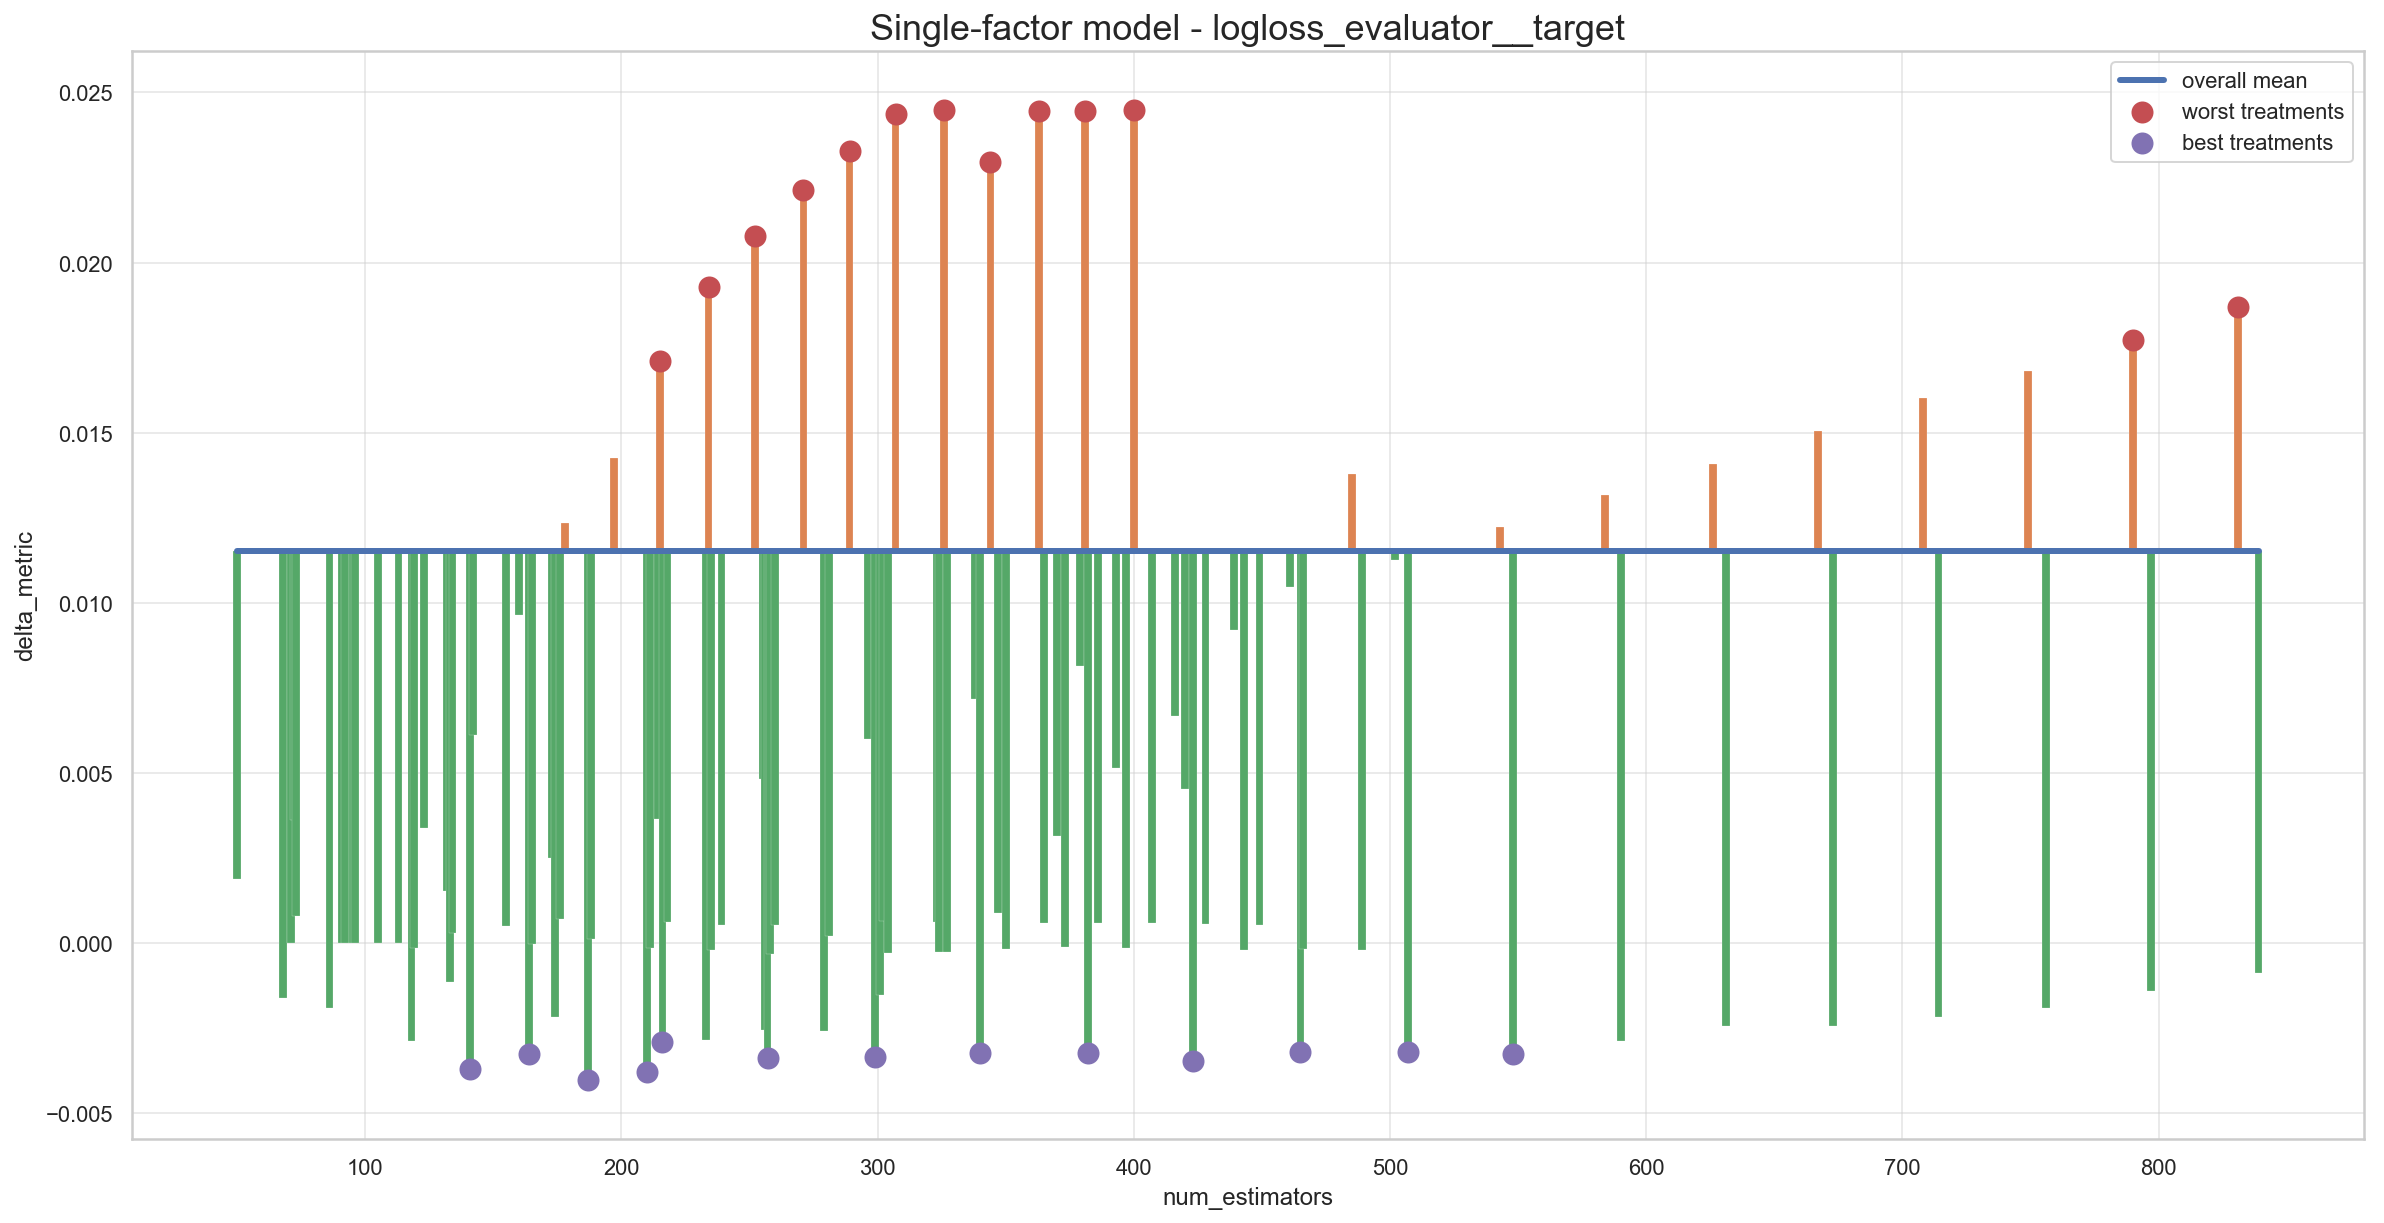
\includegraphics[width=0.9\textwidth]{sfm-cluster1-logloss-ne.png}
    \caption{SFM plot for $\mathcal{S}(C_1, \eta^{(1)}_{NE}, Logloss)$}
    \label{fig:sfm-ne-1}
\end{figure}

\begin{figure}[H]
    \centering
    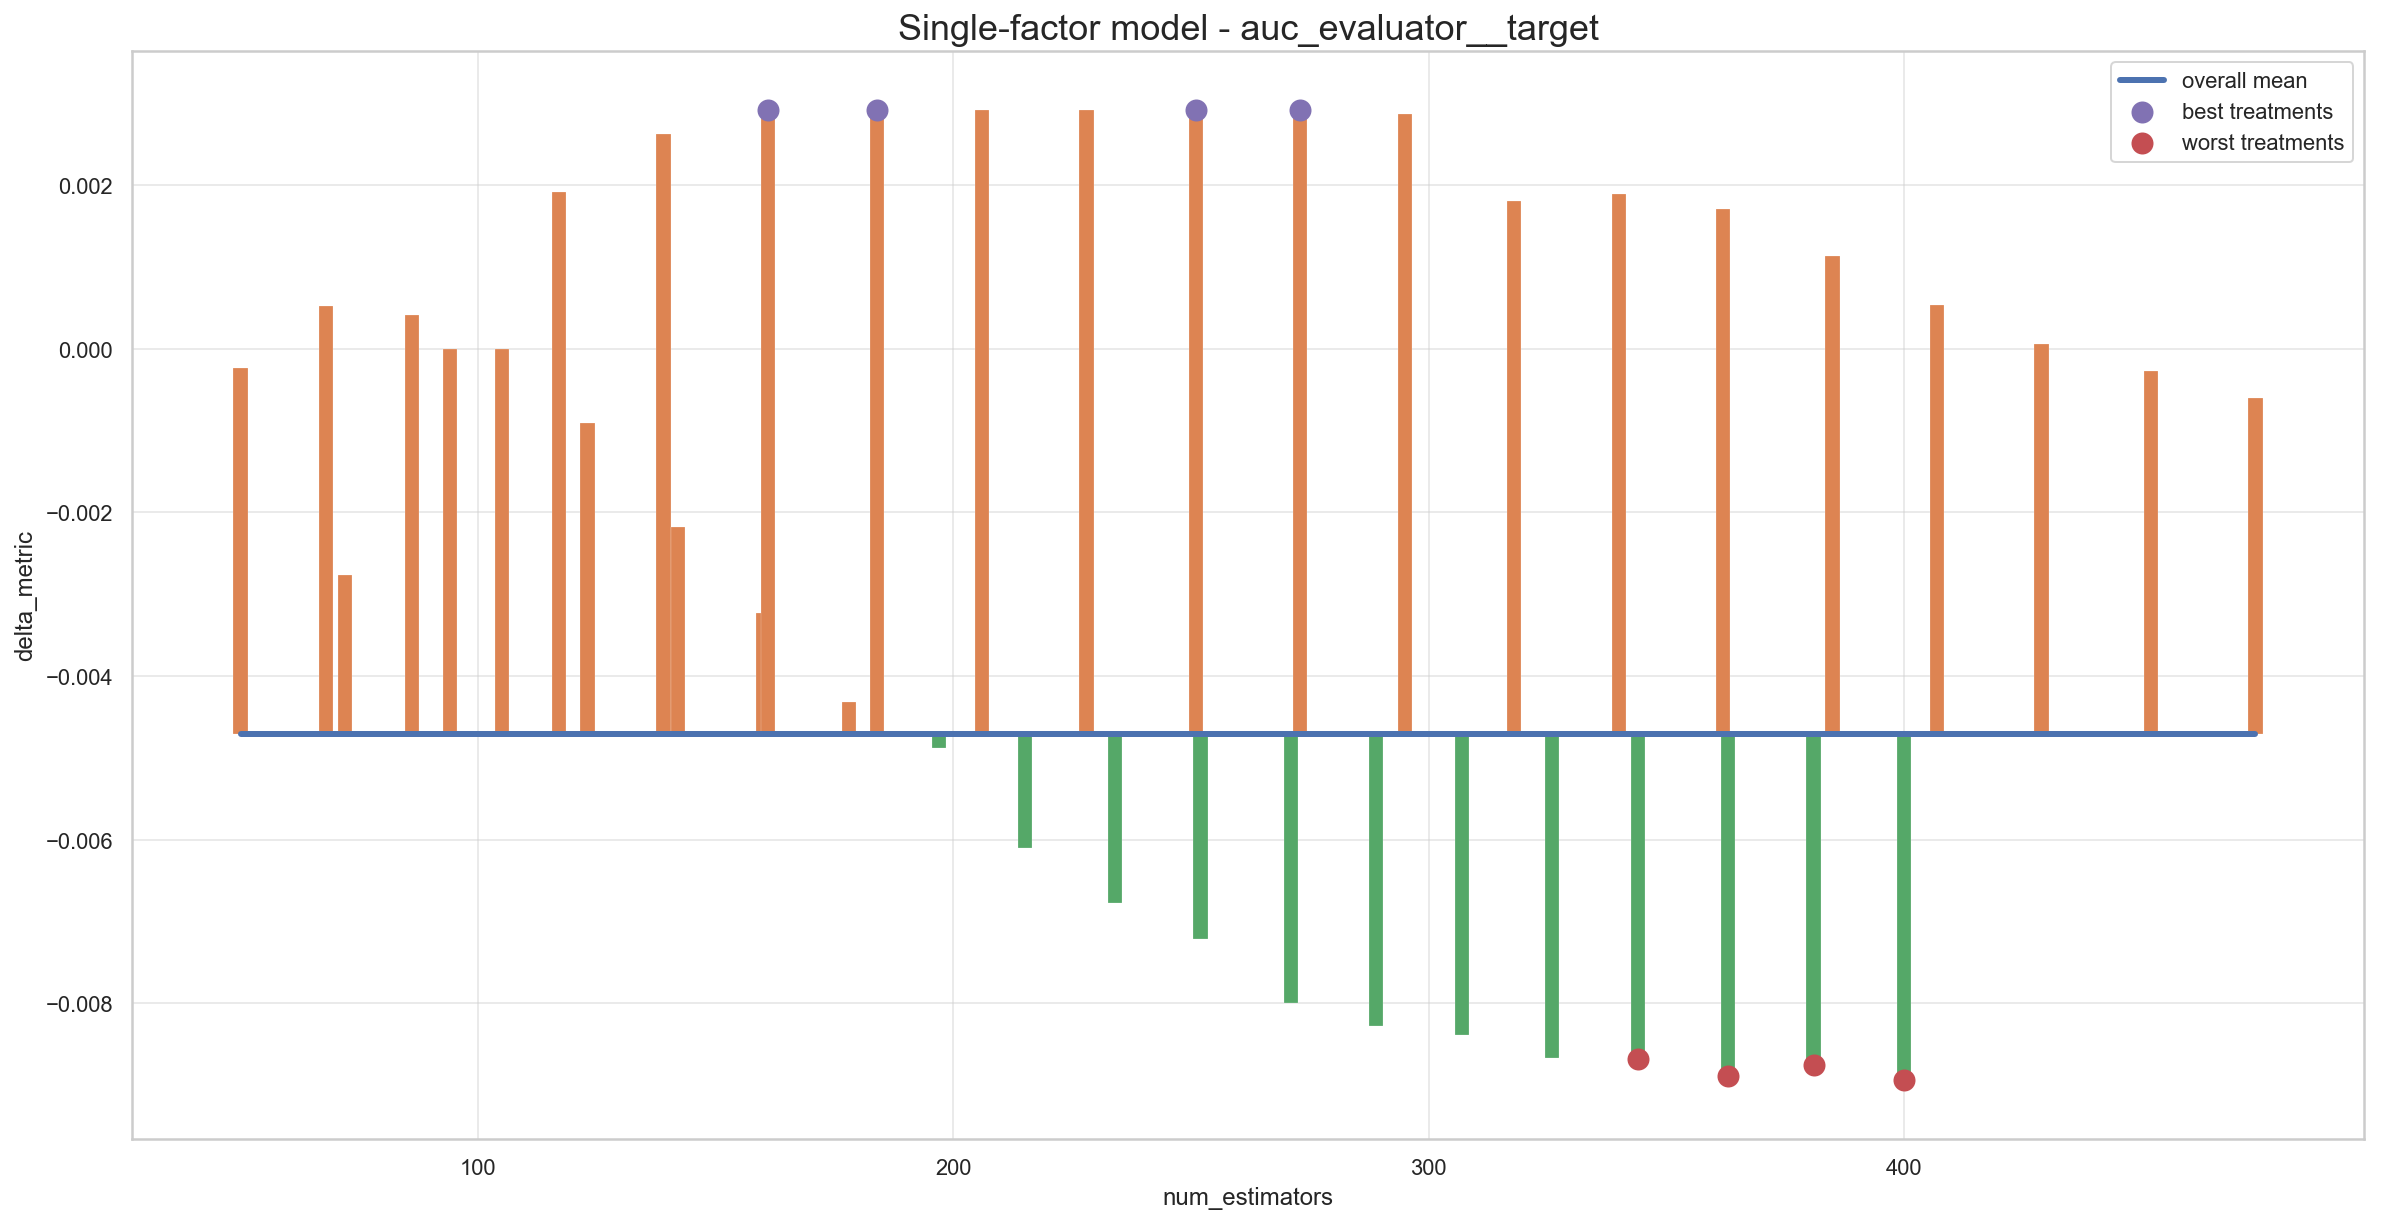
\includegraphics[width=0.9\textwidth]{sfm-cluster6-auc-ne.png}
    \caption{SFM plot for $\mathcal{S}(C_6, \eta^{(6)}_{NE}, AUC)$}
    \label{fig:sfm-ne-2}
\end{figure}

One possible explanation for these results can be that the hyperparameter space chosen for \code{num\_estimators}  (see Subsection \ref{subsec:hp-space-num-est}) didn't cover the most significant values for it. In the results of \cite{probst2018tunability}, the optimal default value for the number of estimators (in their case \code{n\_rounds}) is 4168, and the optimal tuning quantiles $q_5$ and $q_{95}$ for the number of boosting iterations were $920.7$ and $4550.95$, respectively. This means that a good improvement to assess the number of estimators impact is to increase the upper limit in the hyperparameter space of this study to at least $4550$ estimators, using the values from \cite{probst2018tunability}.

\subsection{\texorpdfstring{\Large$\eta_{MD}$}{}}
\label{subsec:analysis-md}

The maximum depth is the individual hyperparameter (i.e. treatments with only one type of hyperparameter being changed) that had the highest significant changes in the performance metrics over all analyzed clusters. The treatment effects are very intuitive and confirm the expected behavior of changing the maximum depth of the trees in machine learning models. This behavior being that small values of maximum depth will limit the model complexity (i.e. it is a form of regularization) and higher values will increase it, which can be seen in Figure \ref{fig:sfm-md-1}.

Very low values of maximum depth generates models with poor performance, which then increases as the maximum depth rises, achieving an ``optimal point''. Then it starts decreasing, probably because the models start to overfit due to high complexity.

\begin{figure}[H]
    \centering
    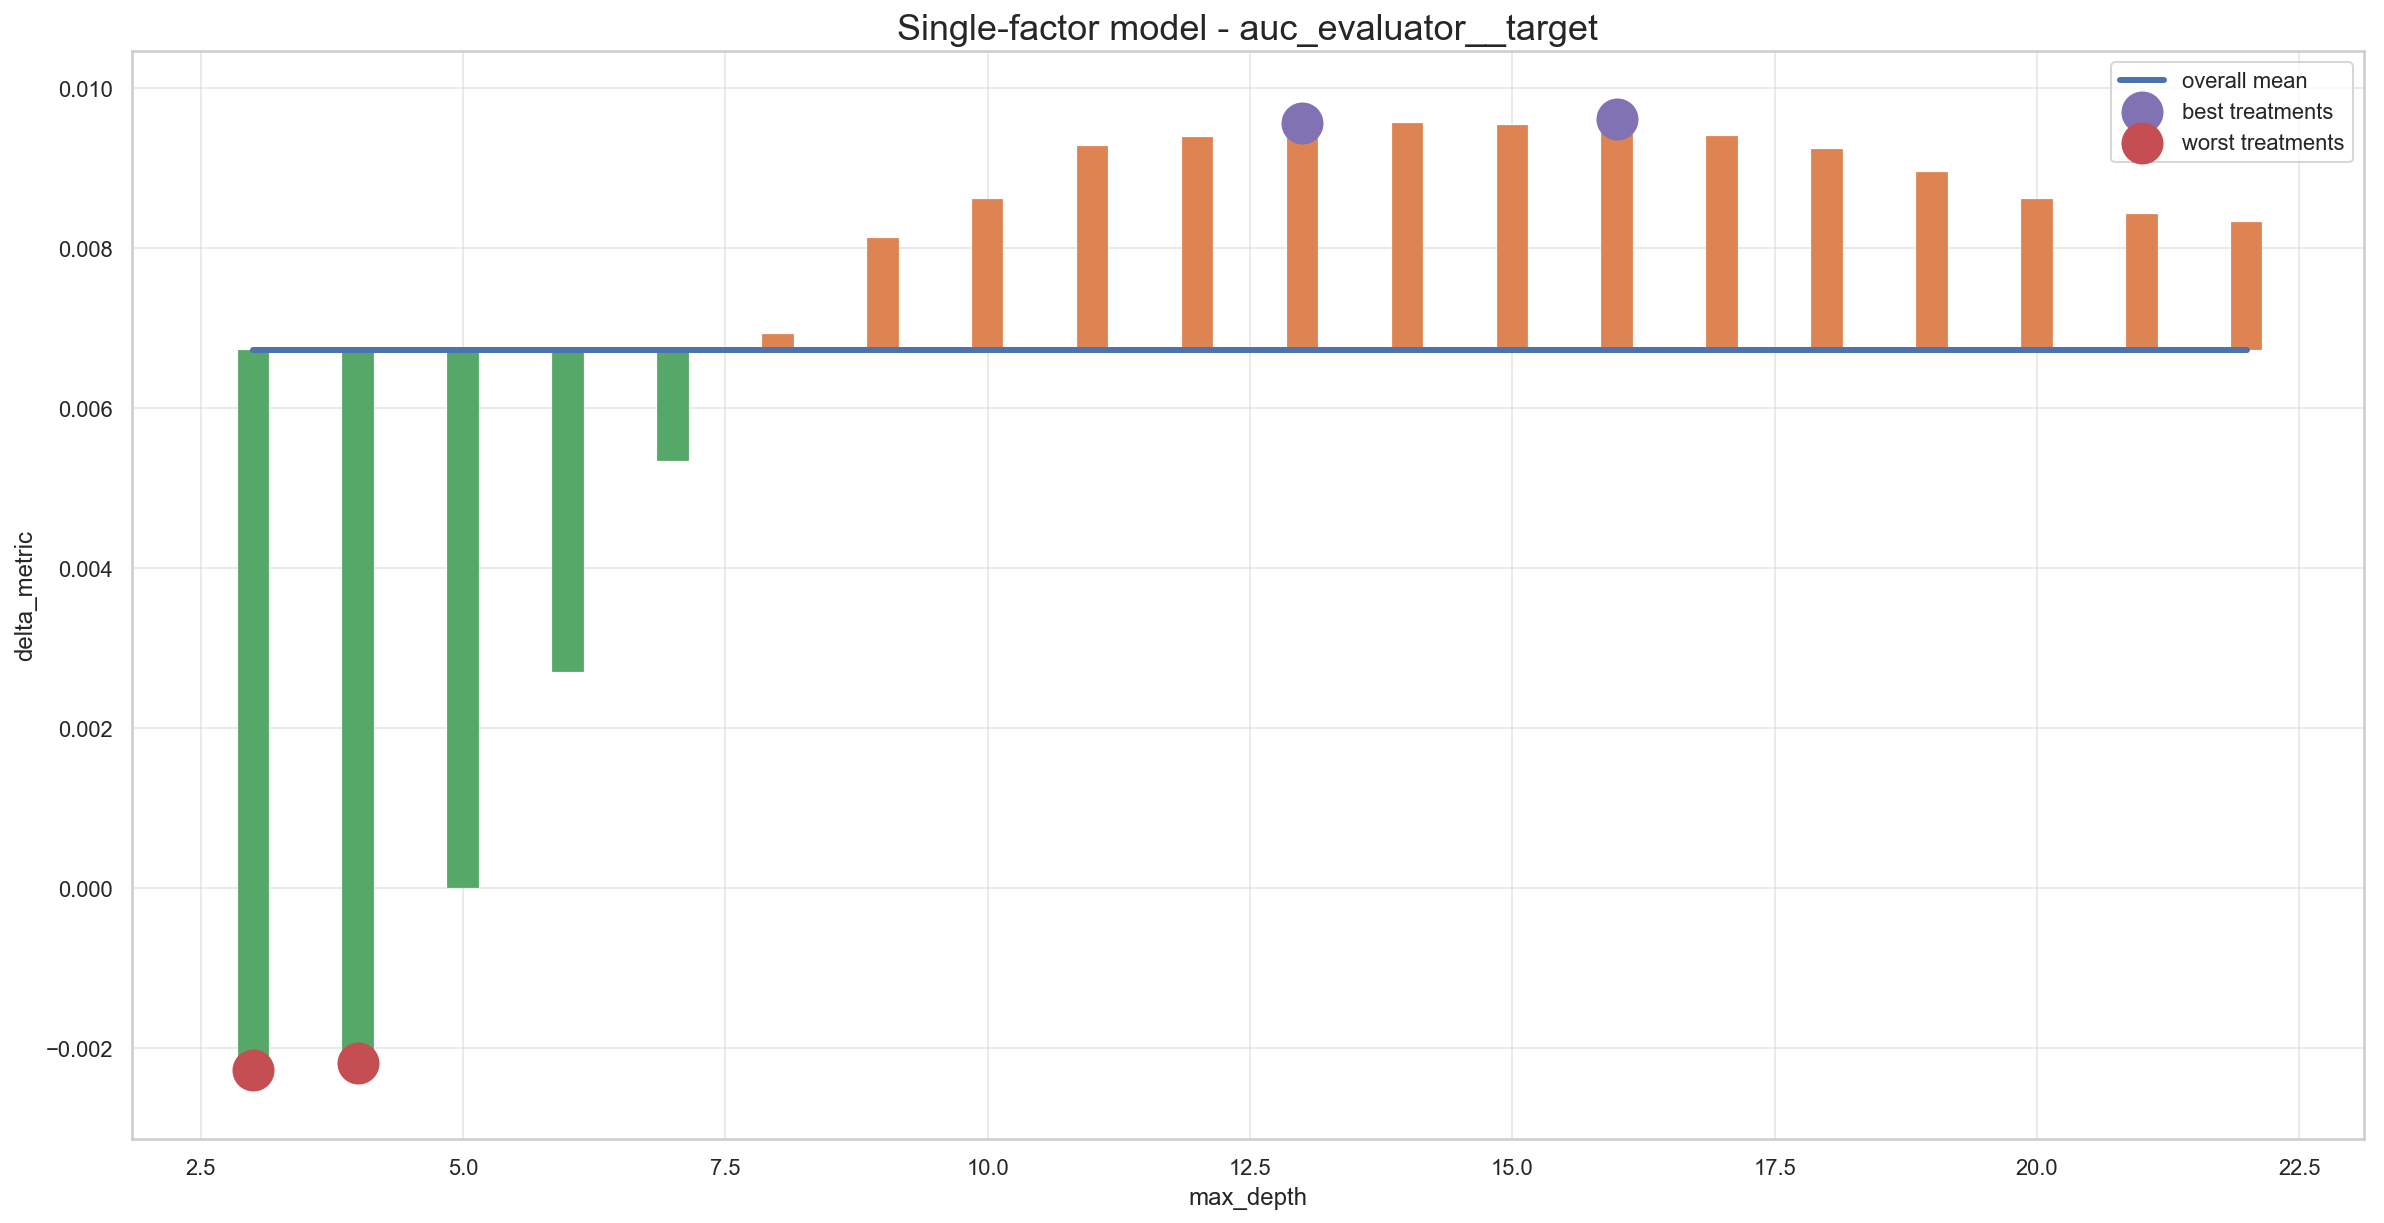
\includegraphics[width=.9\textwidth]{sfm-cluster3-auc-md.png}
    \caption{SFM plot for $\mathcal{S}(C_3, \eta^{(3)}_{MD}, AUC)$}
    \label{fig:sfm-md-1}
\end{figure}


\subsection{\texorpdfstring{\Large$\eta_{LR}$}{}}

The learning rate hyperparameter had a small number of significant results, but when analyzing the absolute value of the experiment's $\hat{\tau_i}$, their overall absolute impact is smaller than $\eta_{MD}$. Increasing the value of the learning is a way to increase the ``steps'' in the \textit{optimization space} of an algorithm. Both the $\delta_{AUC}$ plot and the SFM plot in Figures \ref{fig:delta-auc-cluster3-lr} and \ref{fig:sfm-lr-1} show a similar pattern, where low values of learning rate usually have a worse performance metric than high values of learning rate. This probably happens because all other hyperparameters are kept the same, and the learning rate increases the effect of each boosting iteration, which can yield a better model if the number of boosting iterations (\code{num\_estimators}) is relatively low.

\begin{figure}[H]
    \centering
    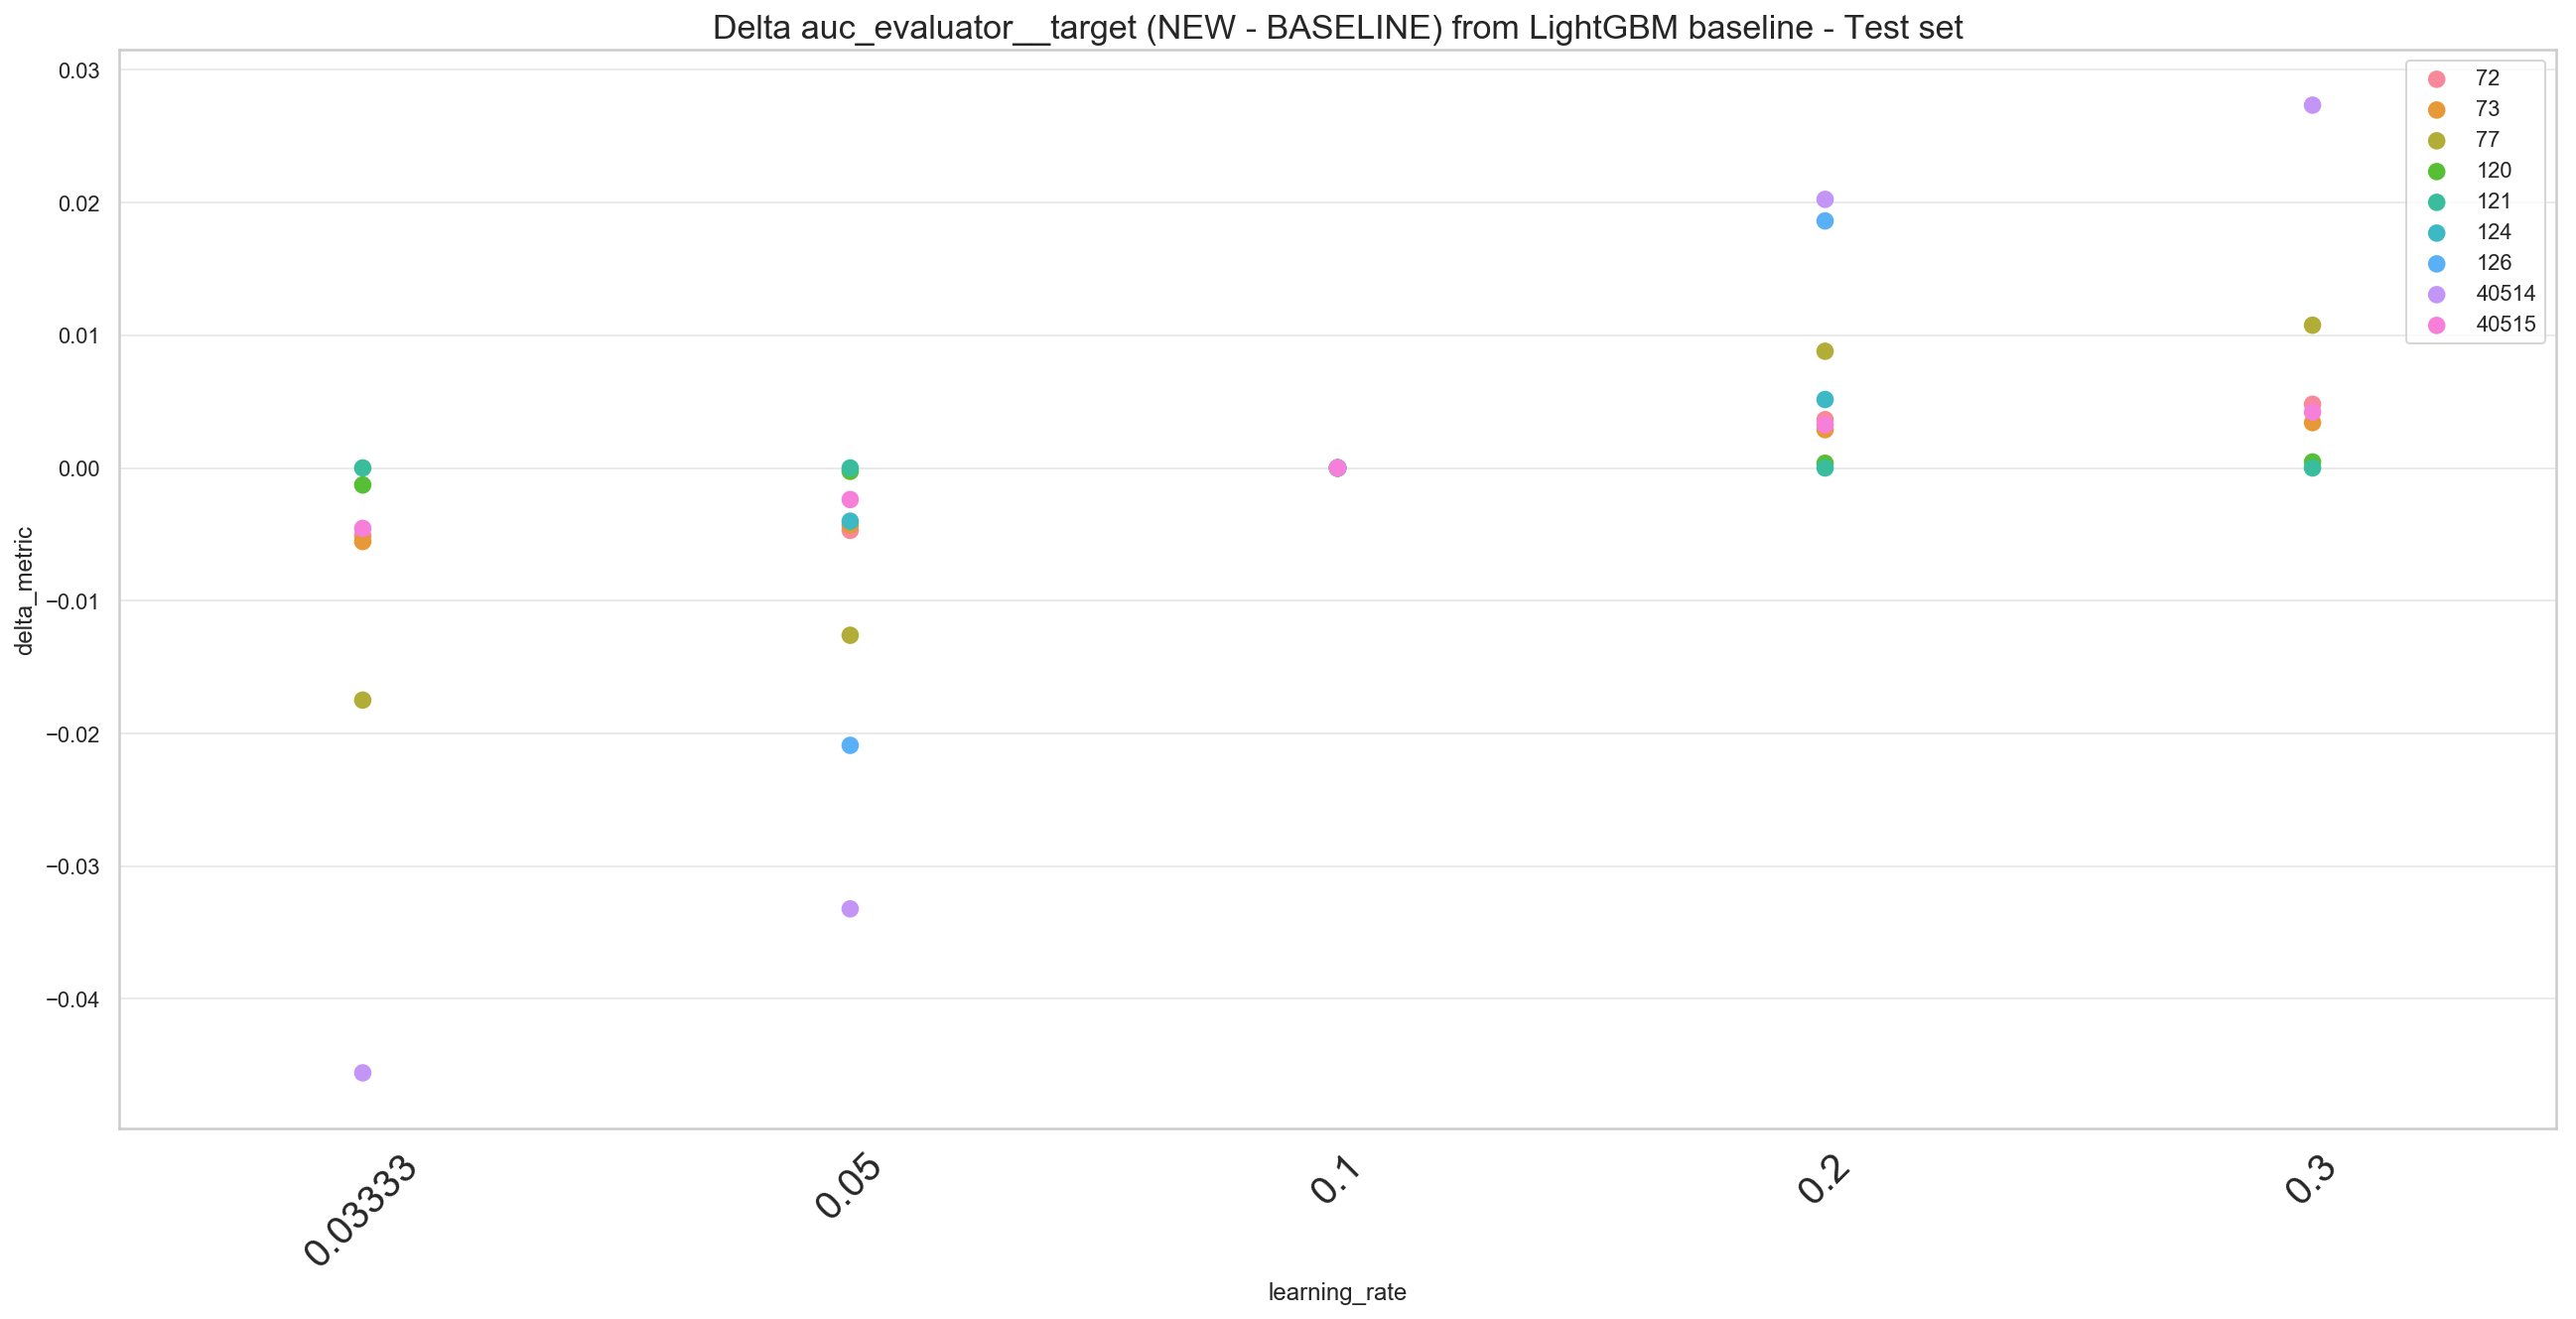
\includegraphics[width=.9\textwidth]{delta_auc-cluster3-lr.png}
    \caption{$\delta_{AUC}$ plot for $\mathcal{S}(C_3, \eta^{(3)}_{LR}, AUC)$}
    \label{fig:delta-auc-cluster3-lr}
\end{figure}

\begin{figure}[H]
    \centering
    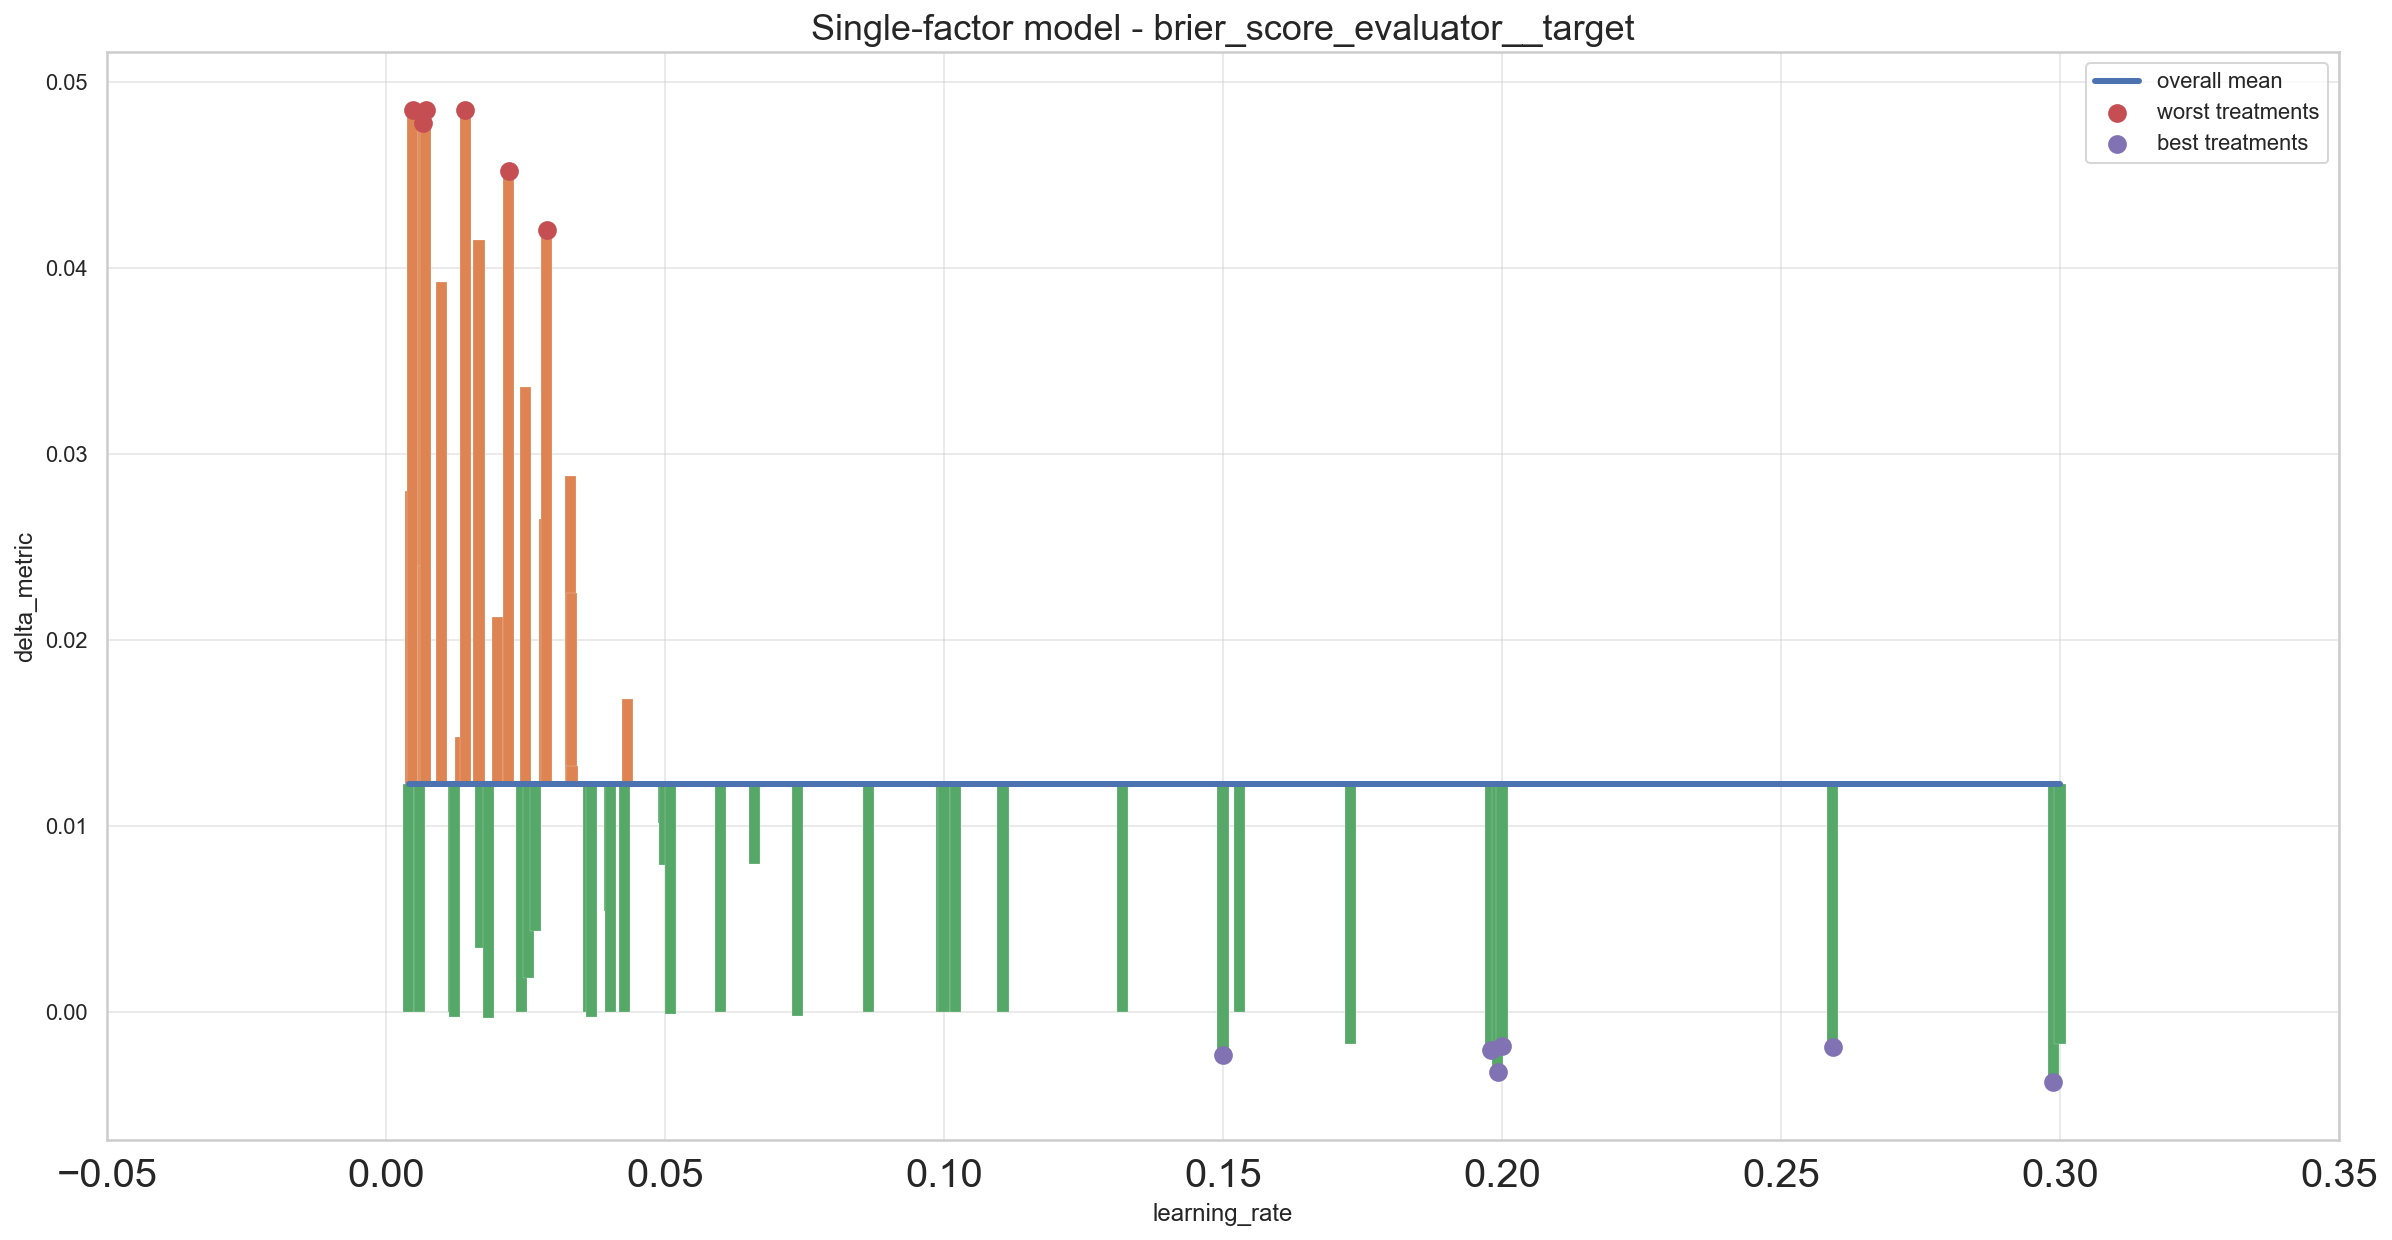
\includegraphics[width=.9\textwidth]{sfm-cluster1-brier-lr.png}
    \caption{SFM plot for $\mathcal{S}(C_1, \eta^{(1)}_{LR}, Brier)$}
    \label{fig:sfm-lr-1}
\end{figure}

Comparing these results with \cite{van2018hyperparameter}, it would be better to use a log scale in this hyperparameter space, instead of a uniformly spaced learning rate values: probably the magnitude of the learning rate values was too small to really observe the full impact of the learning rate individually. Another fact is that some of the learning rate experiments didn't had enough samples when testing their significance, so a possible improvement for future work is to increase the number of learning rates values considered.

\subsection{\texorpdfstring{\Large$\eta_{MD, LR}$}{}}

The combination of changing both the maximum depth and learning rate ($\eta_{MD, LR}$) in the machine learning models is the one combination that had the highest number of significant changes in performance metrics, according to Kruskal–Wallis tests. For instance, 100\% of the scenarios with $\eta_{MD, LR}$ and $\delta_{Brier}$ have had a significant difference in the treatment means, the only hyperparameter combination to do so.


\begin{figure}[H]
    \centering
    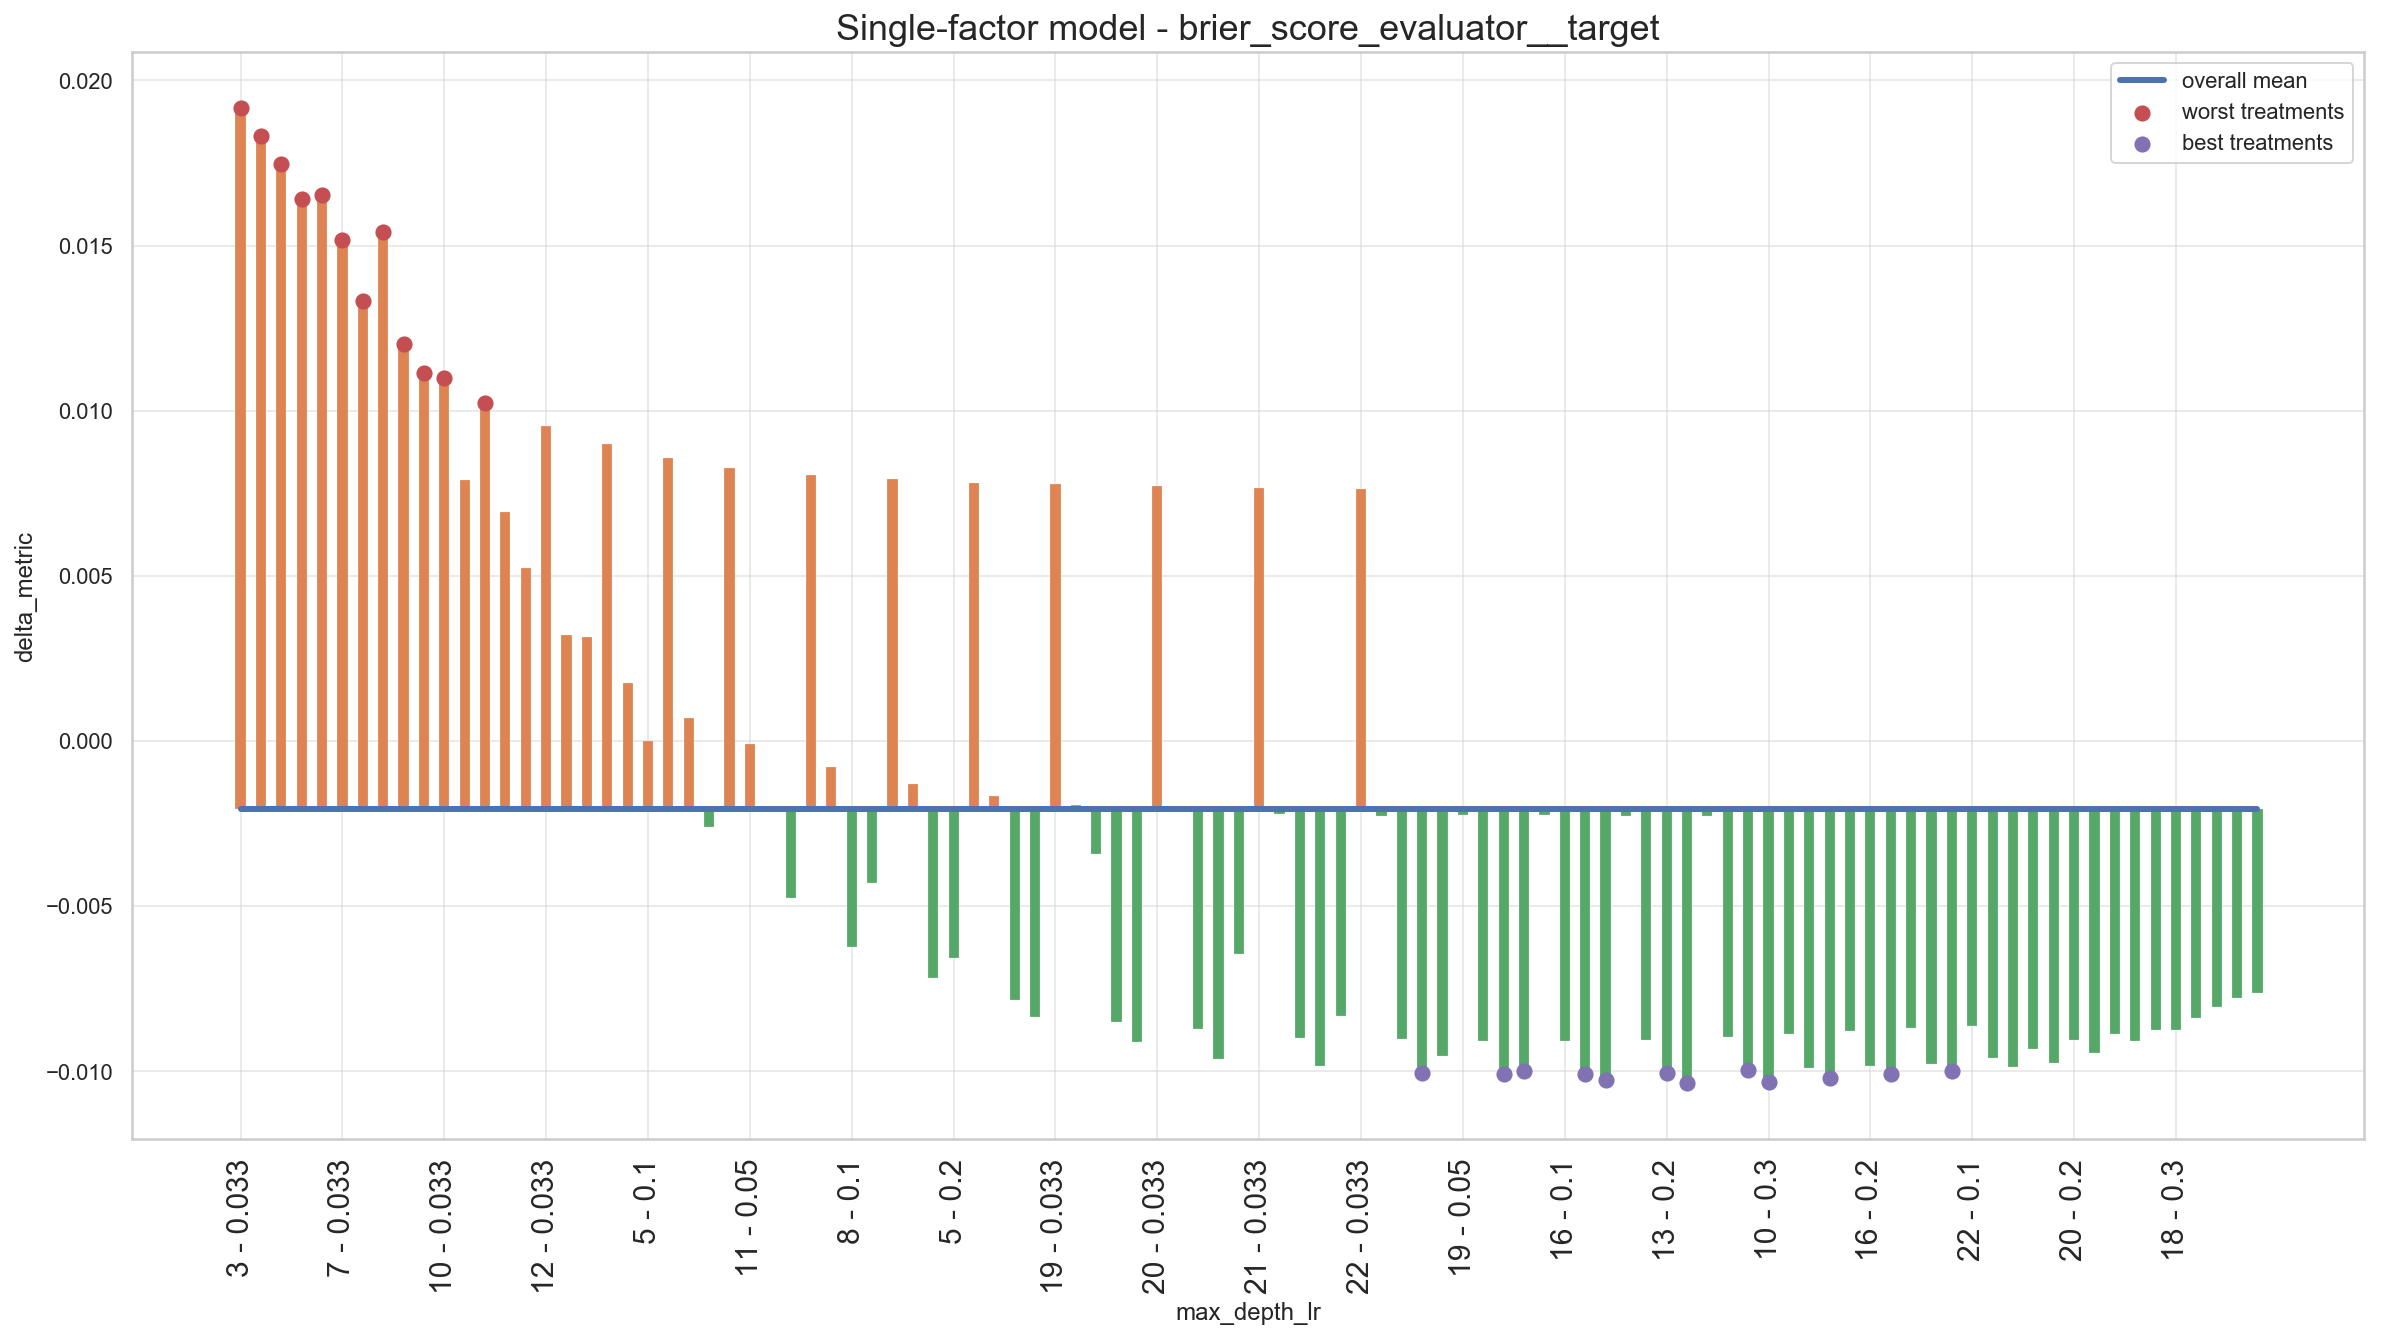
\includegraphics[width=.9\textwidth]{sfm-cluster3-brier-mdlr.png}
    \caption{SFM plot for $\mathcal{S}(C_3, \eta^{(3)}_{MD, LR}, Brier)$}
    \label{fig:sfm-mdlr-1}
\end{figure}

As explained in the last Subsection, the learning rate can increase (or ``accelerate'') the search over the gradient boosting optimization space, and the results shown here confirm this intuition. First, we can observe in Figure \ref{fig:sfm-mdlr-1} and Figure \ref{fig:sfm-mdlr-2} the same behavior found in the SFM plots from the experimental scenarios where the treatments are only the max depth $\eta_{MD}$, albeit reversed because the figures shown here display the Brier Score instead of AUC. The other evidence is that, by looking at the statistical tests results in Table \ref{table:stats-sig}, one can see that all significant experiments for treatment $\eta_{MD}$ are also significant for $\eta_{MD, LR}$, but there's a number of experiments from column $\eta_{MD}$ which aren't significant that became significant when the treatment is $\eta_{MD, LR}$. 


\begin{figure}[H]
    \centering
    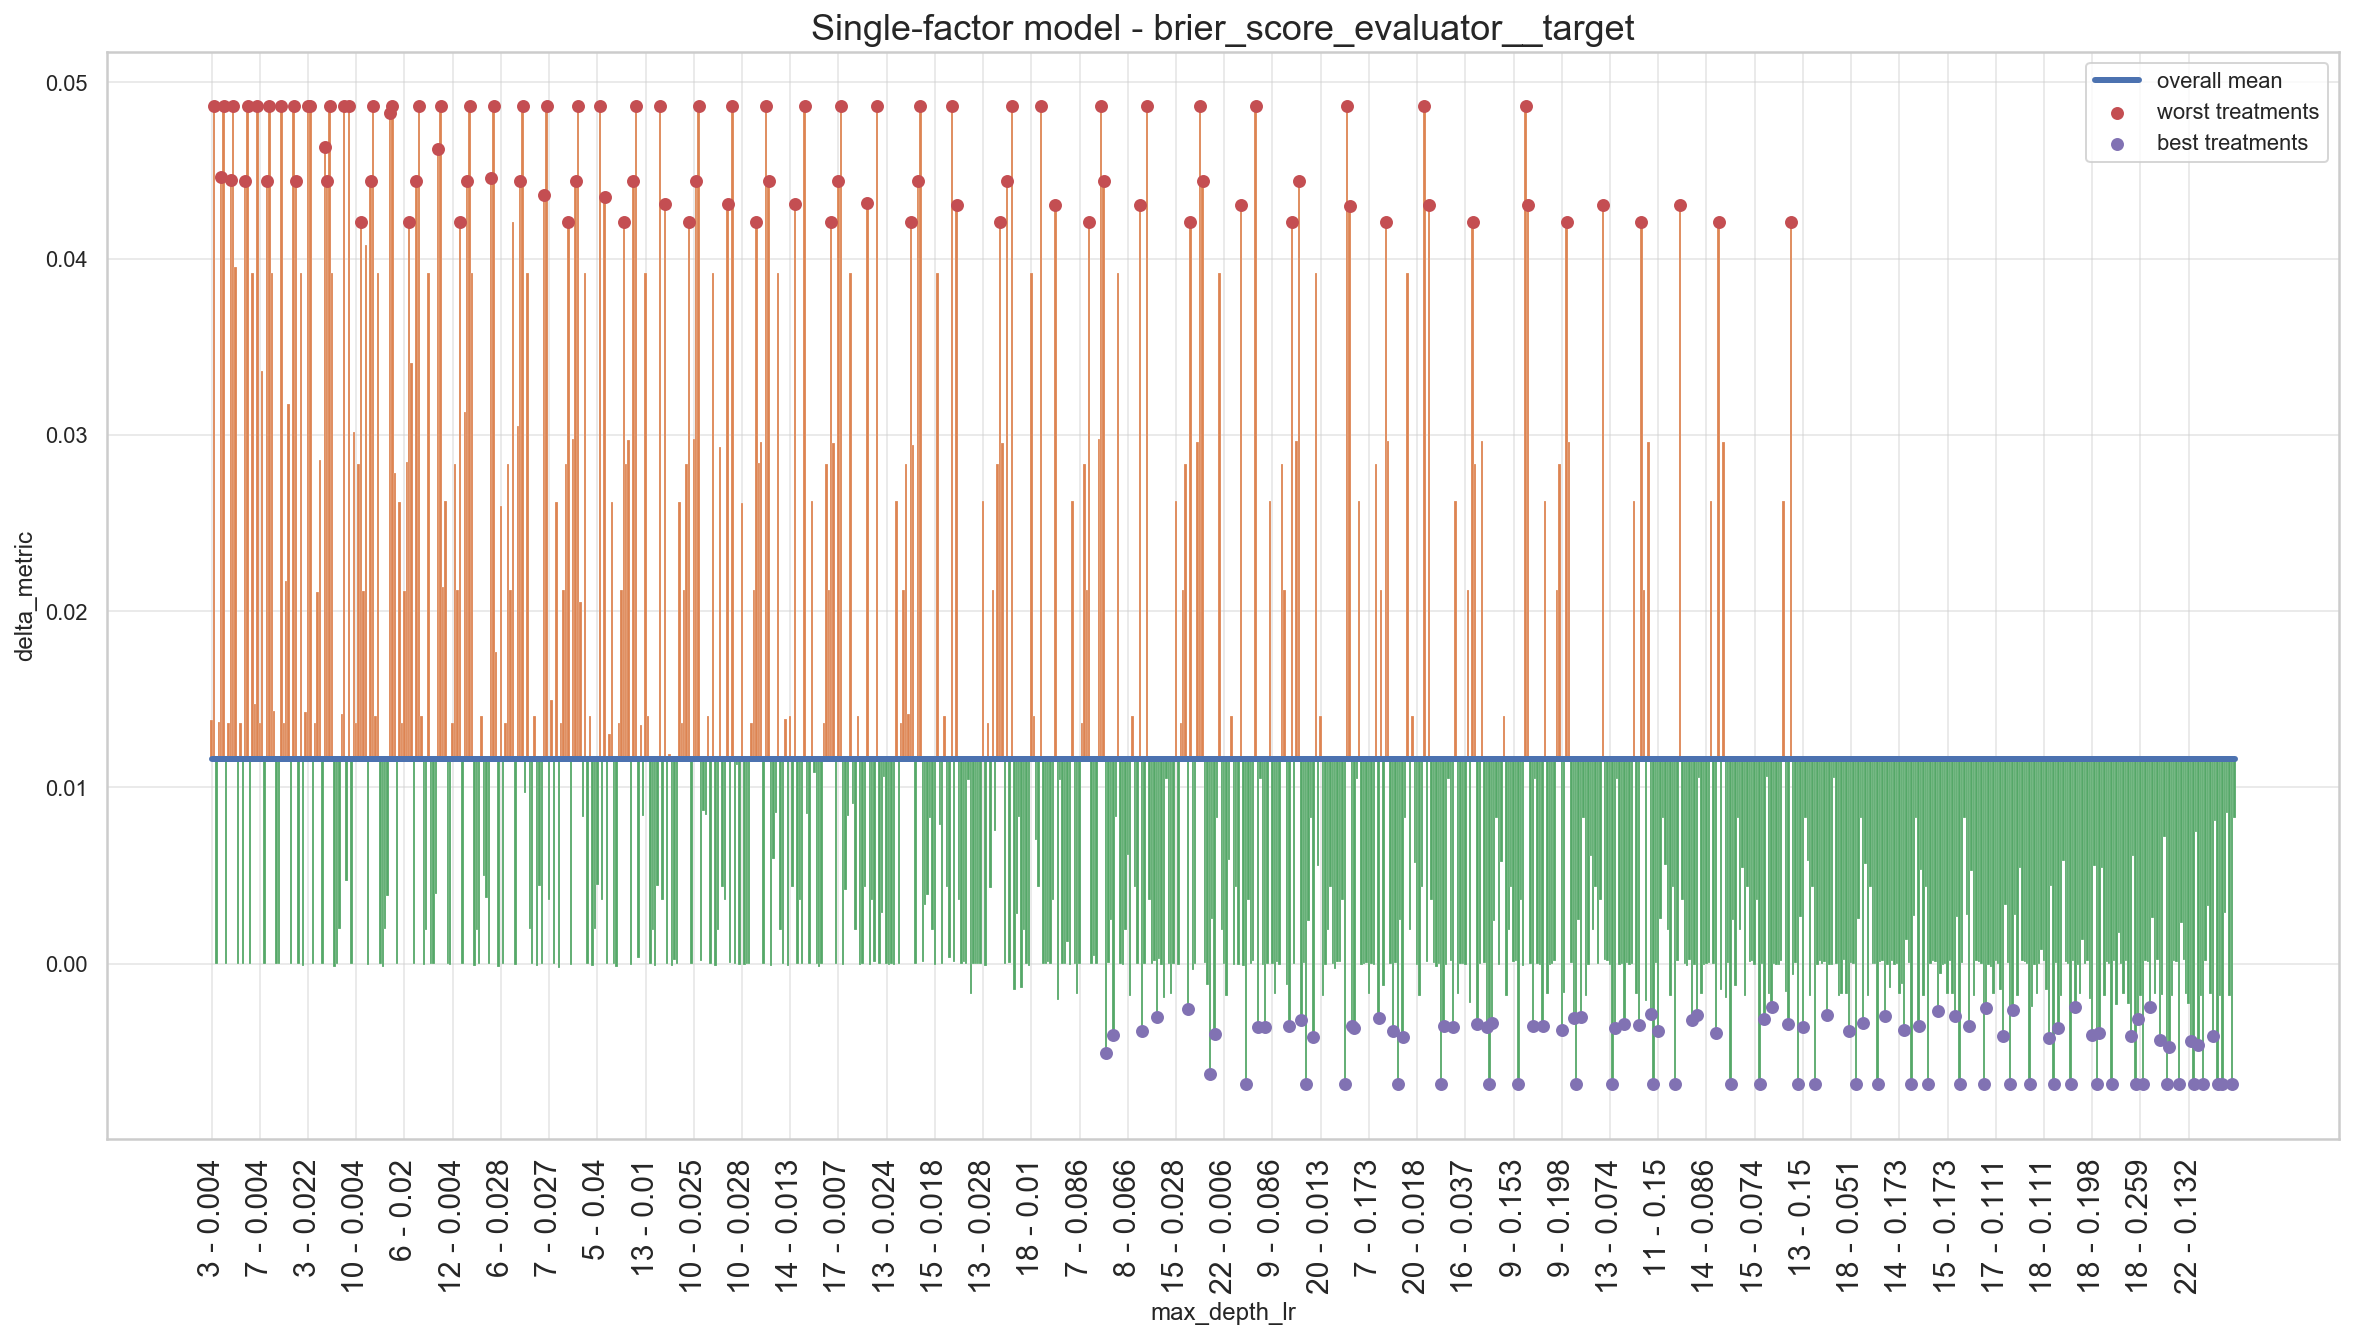
\includegraphics[width=.9\textwidth]{sfm-cluster1-brier-mdlr.png}
    \caption{SFM plot for $\mathcal{S}(C_1, \eta^{(1)}_{MD, LR}, Brier)$}
    \label{fig:sfm-mdlr-2}
\end{figure}

\subsection{\texorpdfstring{\Large$\eta_{MD, NE}$}{}}

This combination of maximum depth and number of estimators had the lowest number of statistically significant experiments: only in two experiments scenarios the null hypothesis of the Kruskal–Wallis test was rejected. This combination, when seen on an individual level (as in Figure \ref{fig:res-mult1}), reveals that possibly treating both maximum depth and number of estimators as a single factor does not captures the overall impact of each hyperparameter. Different approaches might be more useful here, like the \textit{Functional ANOVA} used in \cite{van2018hyperparameter}. Higher limits of the number of estimators distribution could also give a better overall picture of the $\eta_{MD, NE}$, as explained in Subsection \ref{subsec:res-ne}.

However, when analyzing some of the SFM models (even the ones which are heteroscedastic), there's a common pattern in the SFM plots structure. It was explained in \ref{subsec:max-depth} a relationship between max depth and the number of estimators, which describe different ways to change the performance of a classifier based on the magnitude of each hyperparameter.

\begin{figure}[H]
    \centering
    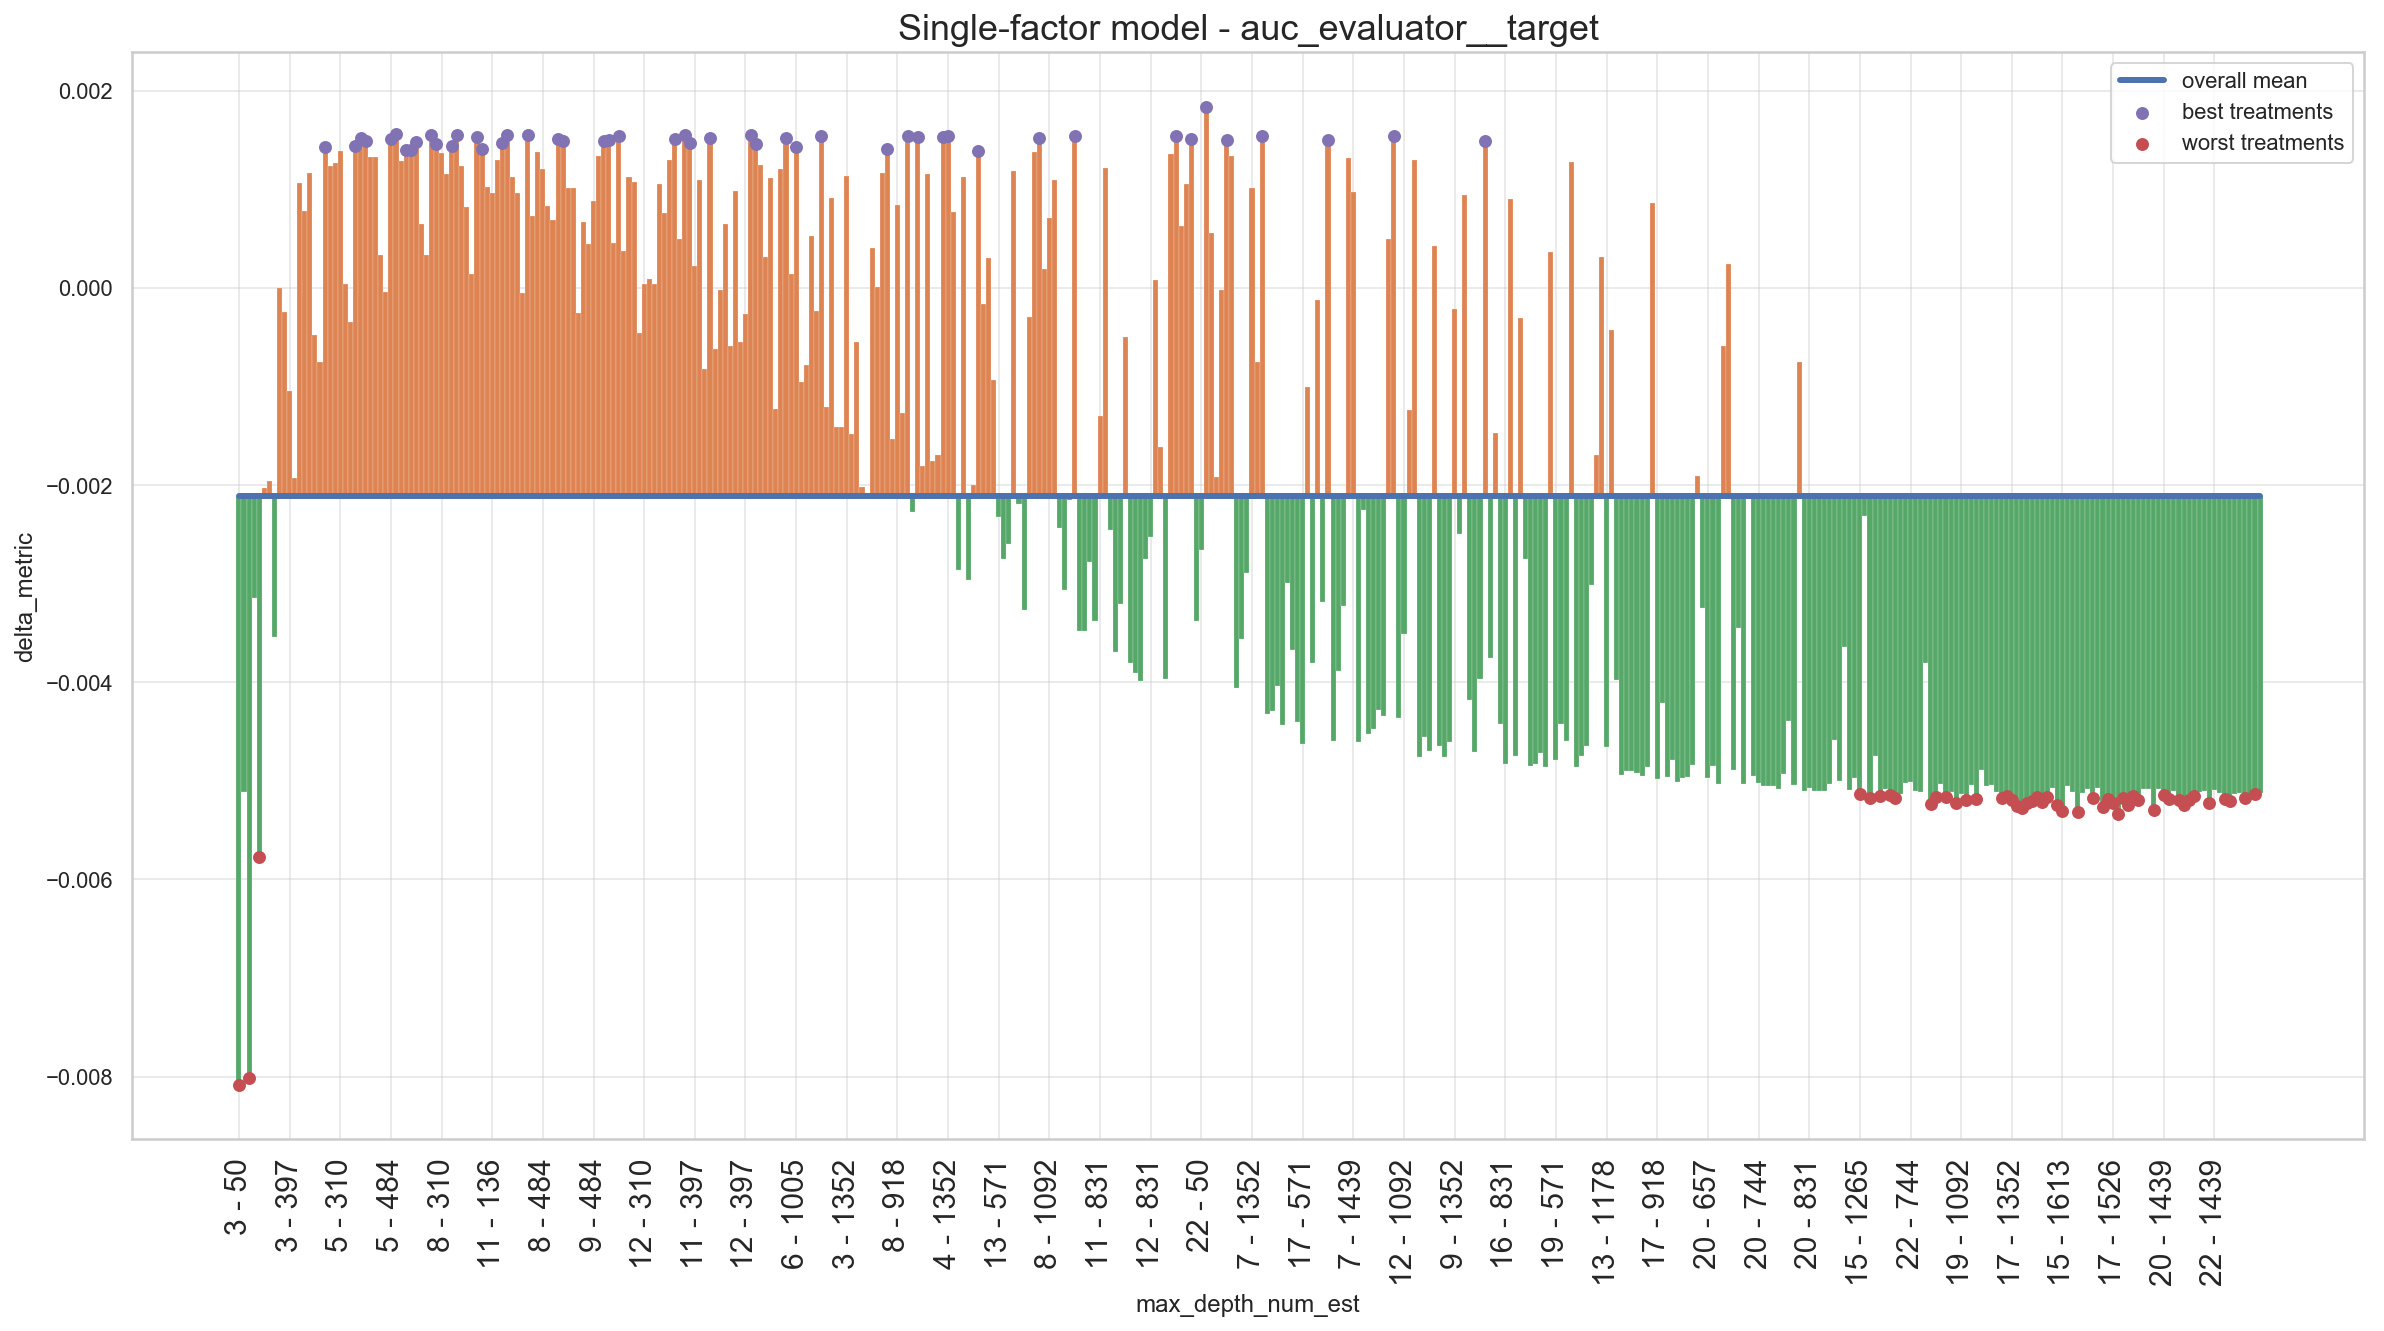
\includegraphics[width=.9\textwidth]{sfm-cluster3-auc-mdne.png}
    \caption{SFM plot for $\mathcal{S}(C_3, \eta^{(3)}_{MD, NE}, AUC)$}
    \label{fig:sfm-mdne-2}
\end{figure}

The same pattern observed in Figure \ref{fig:res-mult1} can be recognized in the SFM plots of the experiments with treatments $\eta_{MD, NE}$. In Figure \ref{fig:sfm-mdne-2} for example, lower values of both \code{max\_depth} and \code{num\_estimators} decreases the AUC, then the AUC increases when there's an equilibrium between both hyperparameter values (the  \textcolor{orange}{orange} section). Finally, the AUC starts decreasing again when both hyperparameter values have high values. There's also a ``middle ground'' where the estimated treatment effects are intercalating, which is an effect of the ordering defined in Subsection \ref{subsec:ordering}: combinations with an average value of maximum depth or number of estimators can increase or decrease the AUC with high variance, which produces the intercalating effect clearly seen in Figure \ref{fig:sfm-mdne-1}.

\begin{figure}[H]
    \centering
    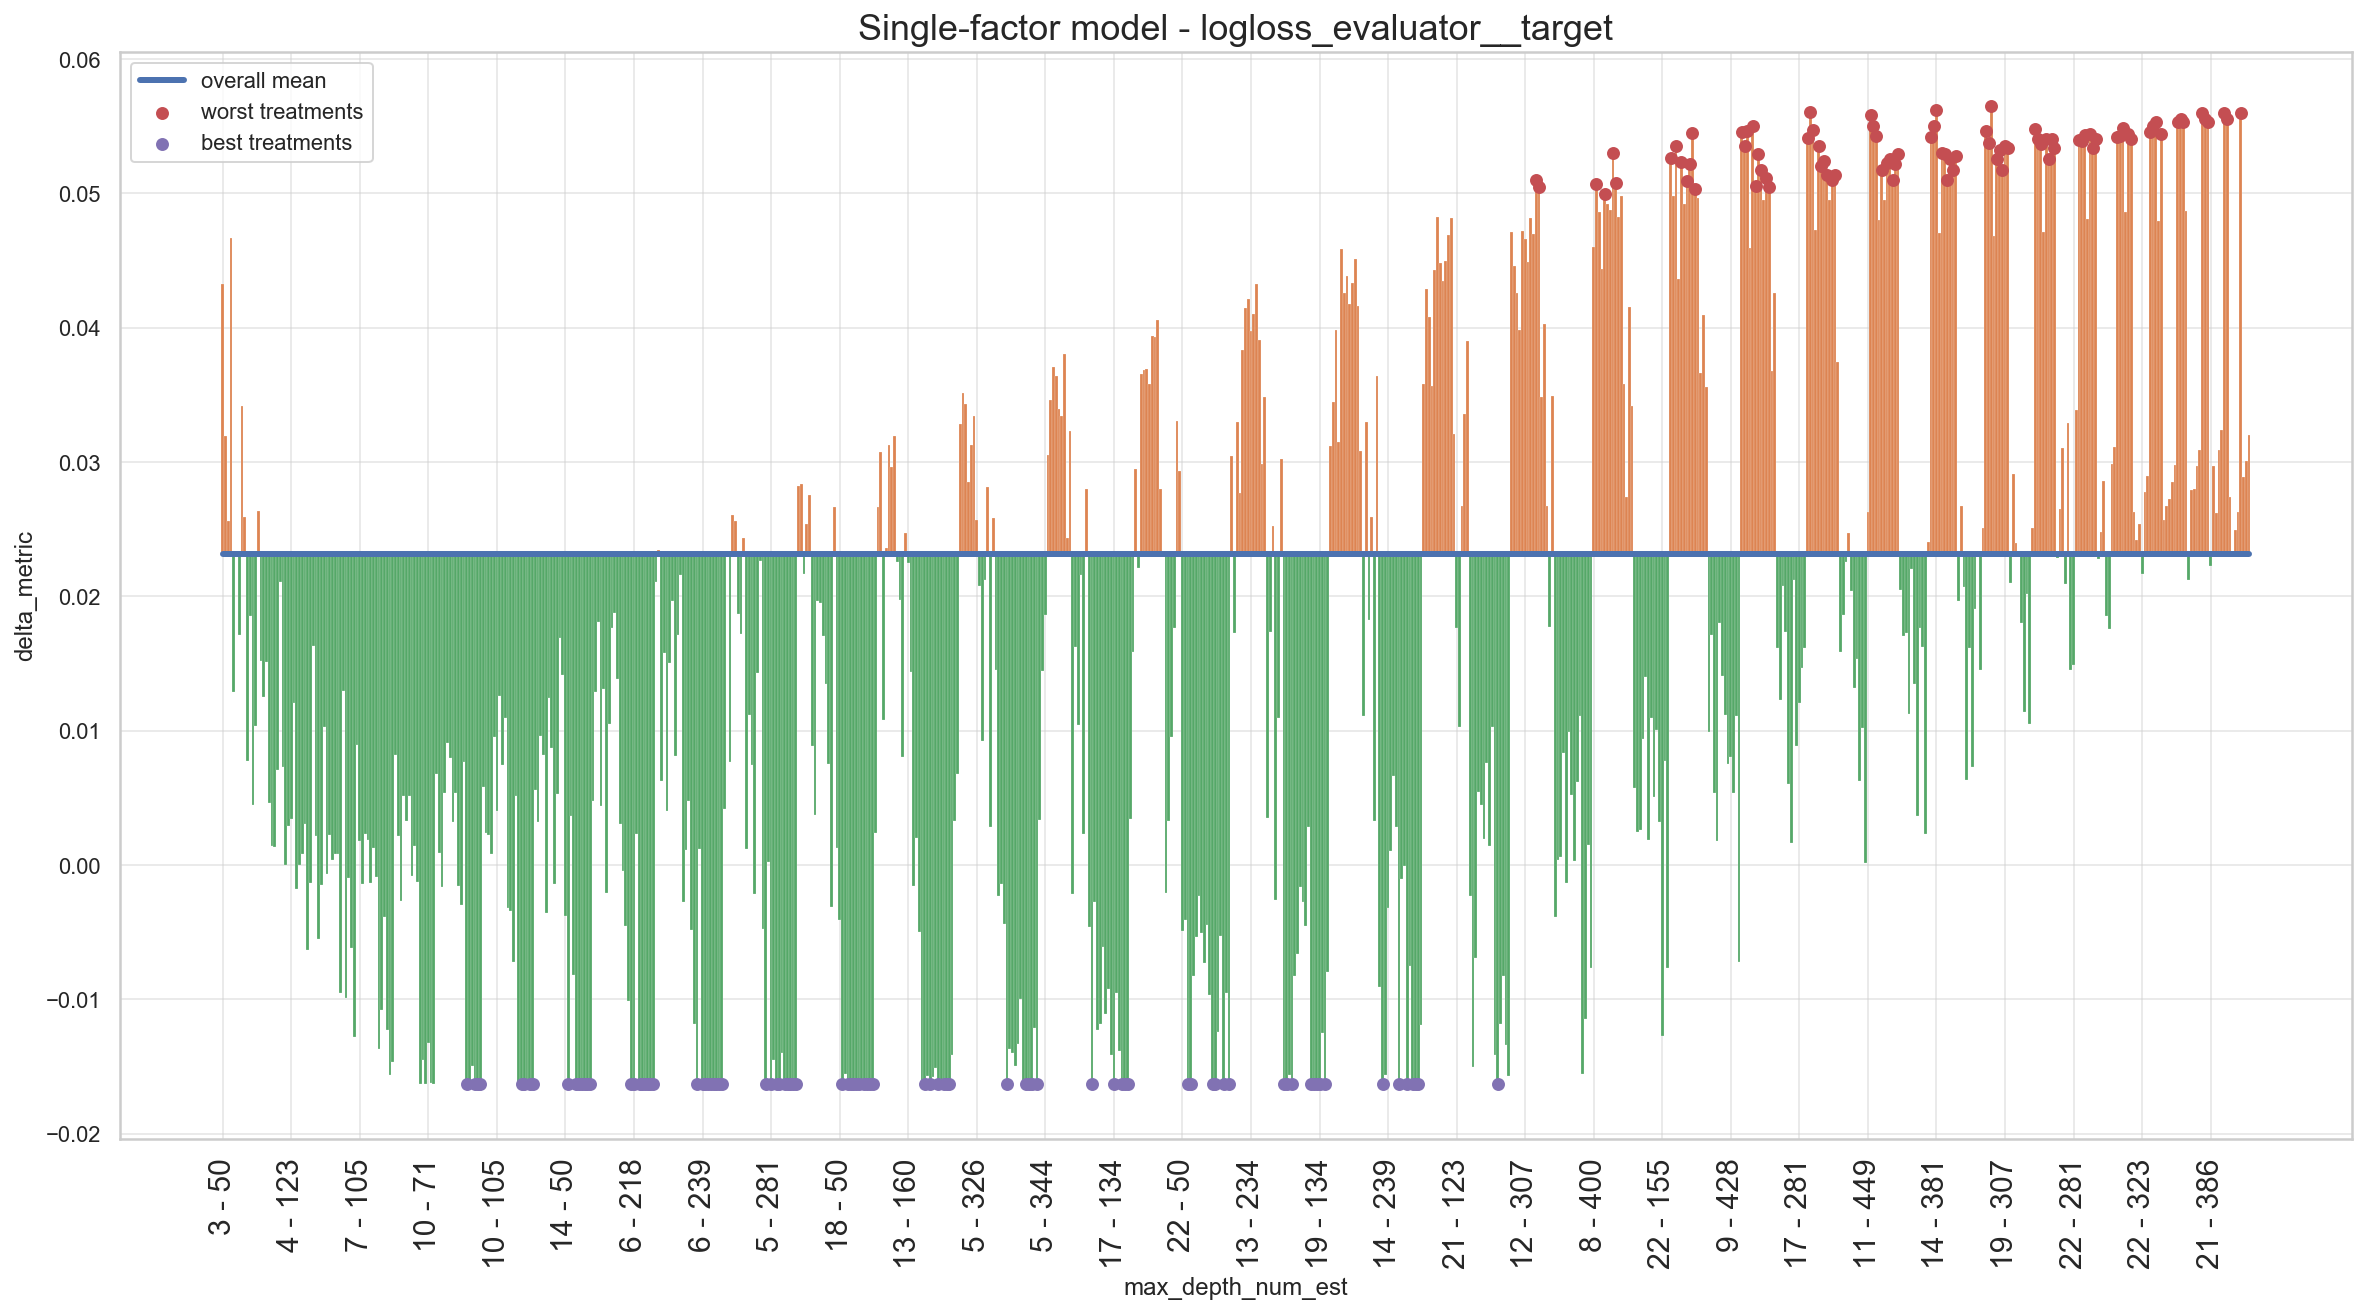
\includegraphics[width=.9\textwidth]{sfm-cluster2-logloss-mdne.png}
    \caption{SFM plot for $\mathcal{S}(C_2, \eta^{(2)}_{MD, NE}, Logloss)$}
    \label{fig:sfm-mdne-1}
\end{figure}

\subsection{\texorpdfstring{\Large$\eta_{LR, NE}$}{}}

The combination of learning rate and number of estimators yield a similar result to $\eta_{MD, LR}$, with more statistically significant results than individually changing either learning rate or number of estimators individually. The SFM plots from these scenarios follow a $\cup$-shaped pattern for AUC , and the opposite $\cap$-shaped pattern for Brier Score (Figure \ref{fig:sfm-lrne-1}) and Logloss results.

The result is also intuitive, because on one hand a small number of boosting iterations coupled with a small learning rate will likely lead to a very simple gradient boosting model, with low performance on the test set. On the other hand, high values of both learning rate and number of estimators can also generate bad classifiers. In the middle section of the SFM plot there's the highest density of the best treatments, which equilibrate both hyperparameter values.

\begin{figure}[H]
    \centering
    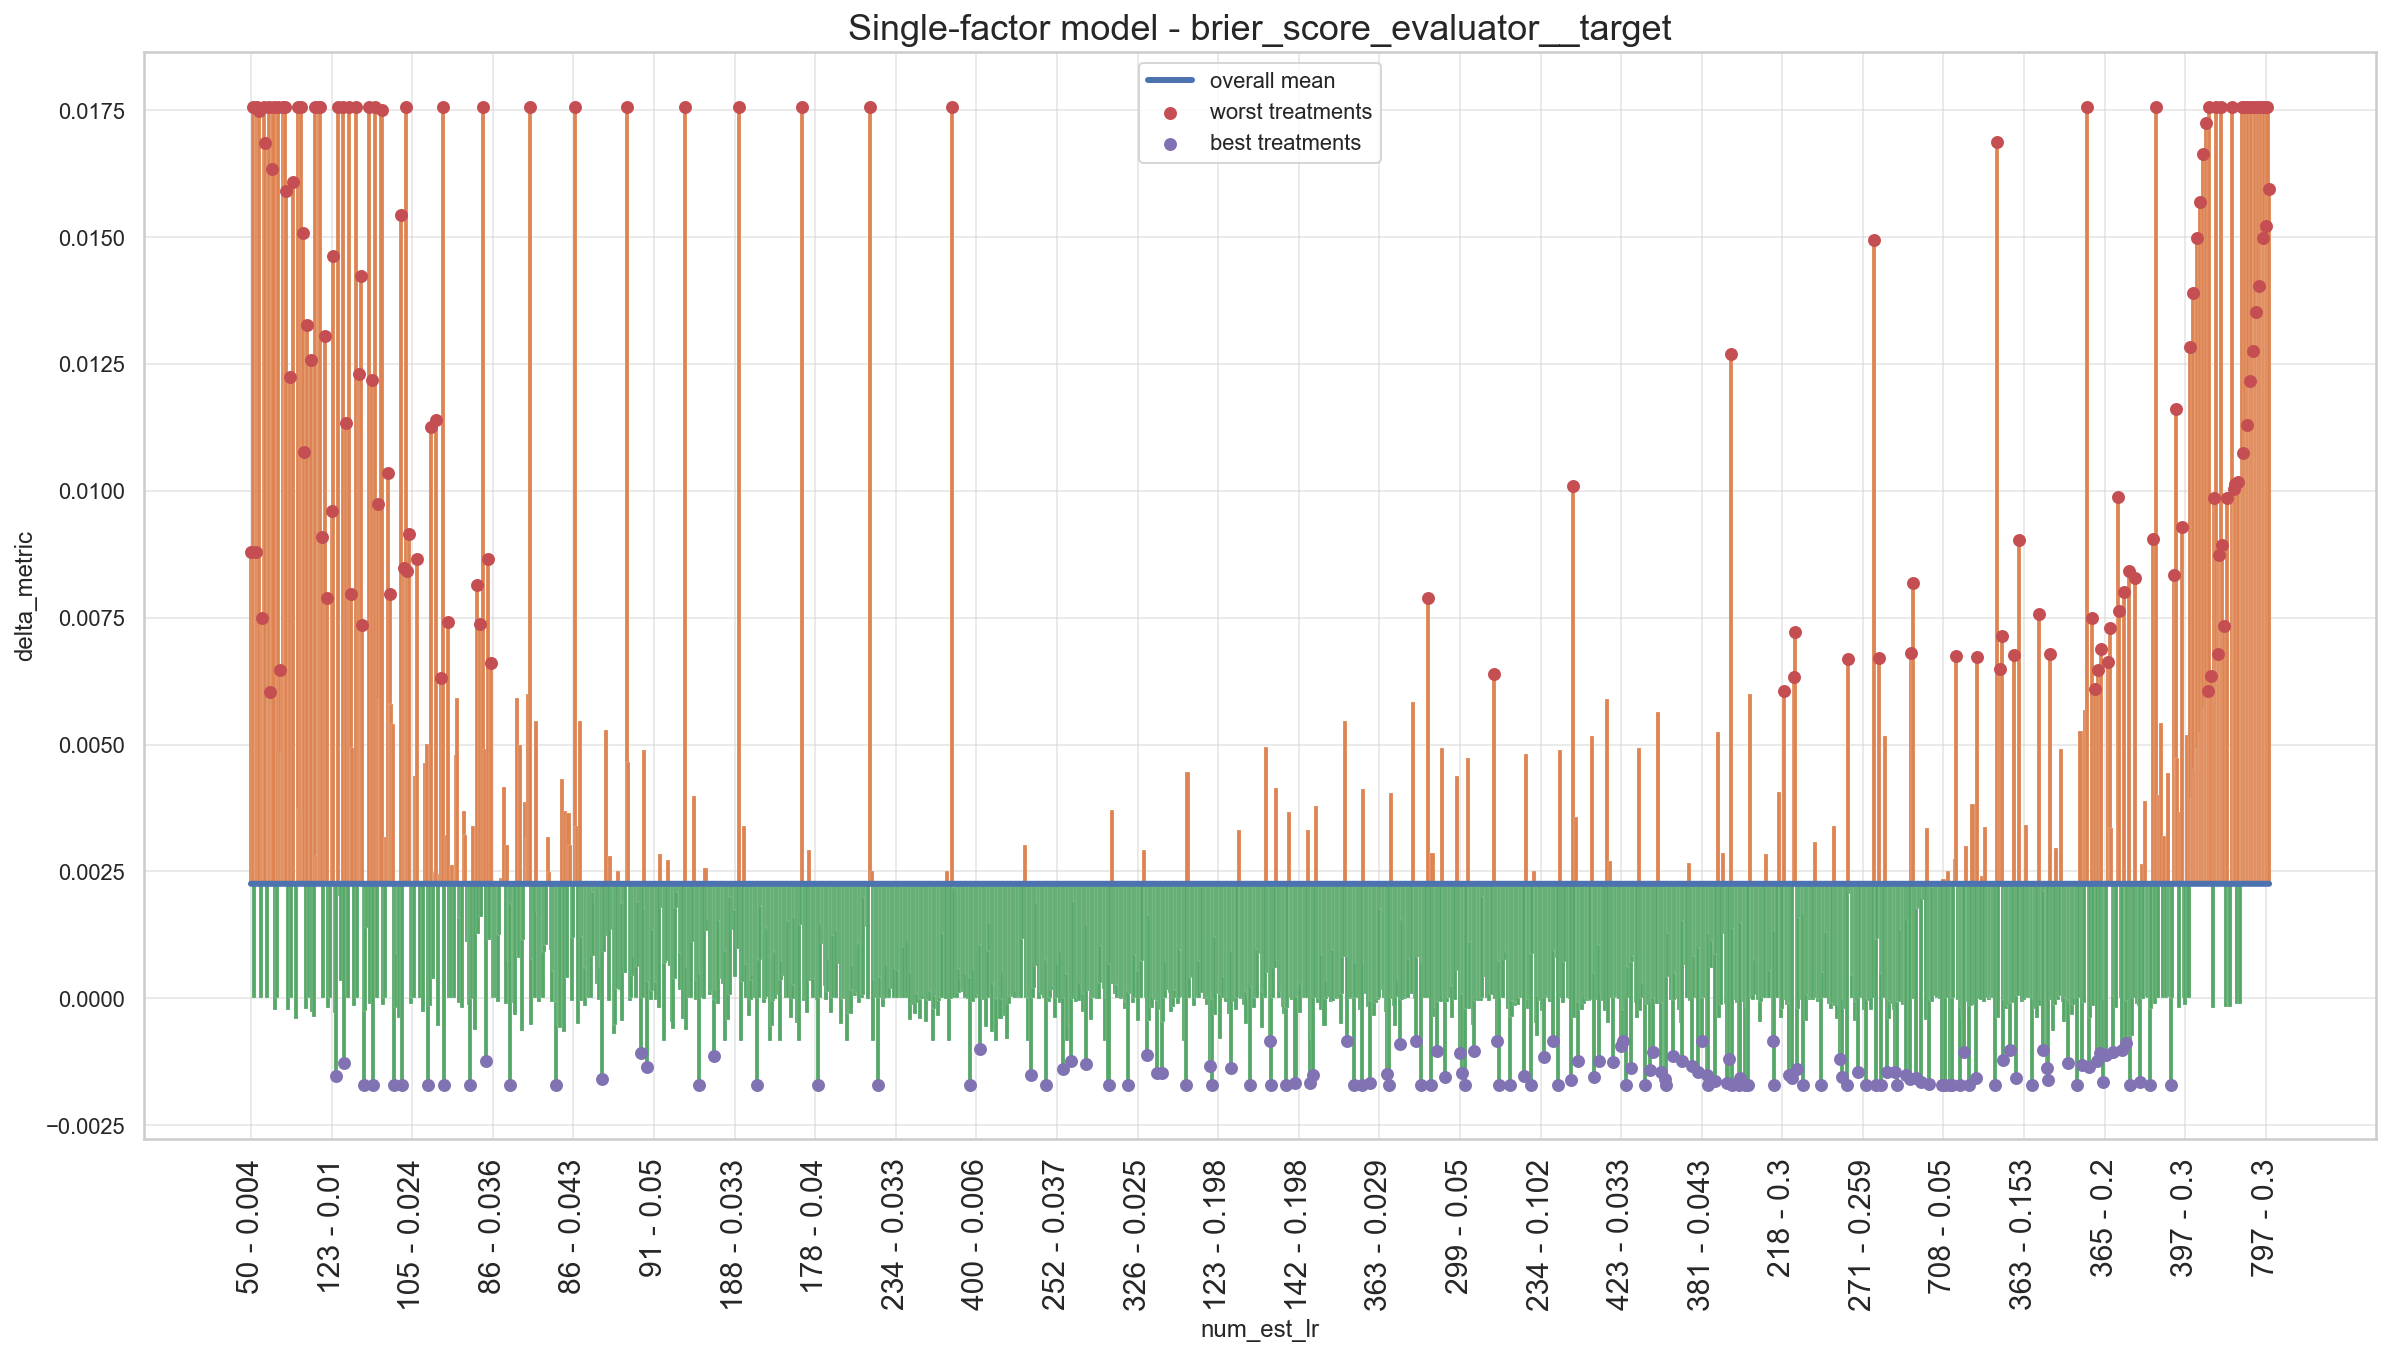
\includegraphics[width=.9\textwidth]{sfm-cluster1-brier-nelr.png}
    \caption{SFM plot for $\mathcal{S}(C_1, \eta^{(1)}_{LR, NE}, Brier)$}
    \label{fig:sfm-lrne-1}
\end{figure}

\subsection{\texorpdfstring{\Large$\eta_{NE, MD, LR}$}{}}

There's a high proportion of single-factor models of experimental scenarios with $\eta_{NE, MD, LR}$ that are significant. If not taking into account the homoscedasticity violations from Cluster 3 data, this would be the combination with the highest number of significant experiments.

Even though this combination has a high impact on the performance metrics, it is harder to visualize a pattern in the SFM plots due to the high dimensionality of the data. There's a clear pattern throughout all cluster results, although some behaviors can be interpreted from it. Figure \ref{fig:delta-nemdlr-1} illustrates the $\delta_{Logloss}$ plot for all treatment values of $\eta_{NE, MD, LR}$ for Cluster 2, with the respective SFM plot in Figure \ref{fig:sfm-nemdlr-1}: there's a similar $\cup$-shaped pattern as in the $\eta_{LR, NE}$ combinations, but in this case this pattern does not consistently appear in the other clusters experimental results.

% yes, the cluster is 2, there's a typo in the image filename =(
\begin{figure}[H]
    \centering
    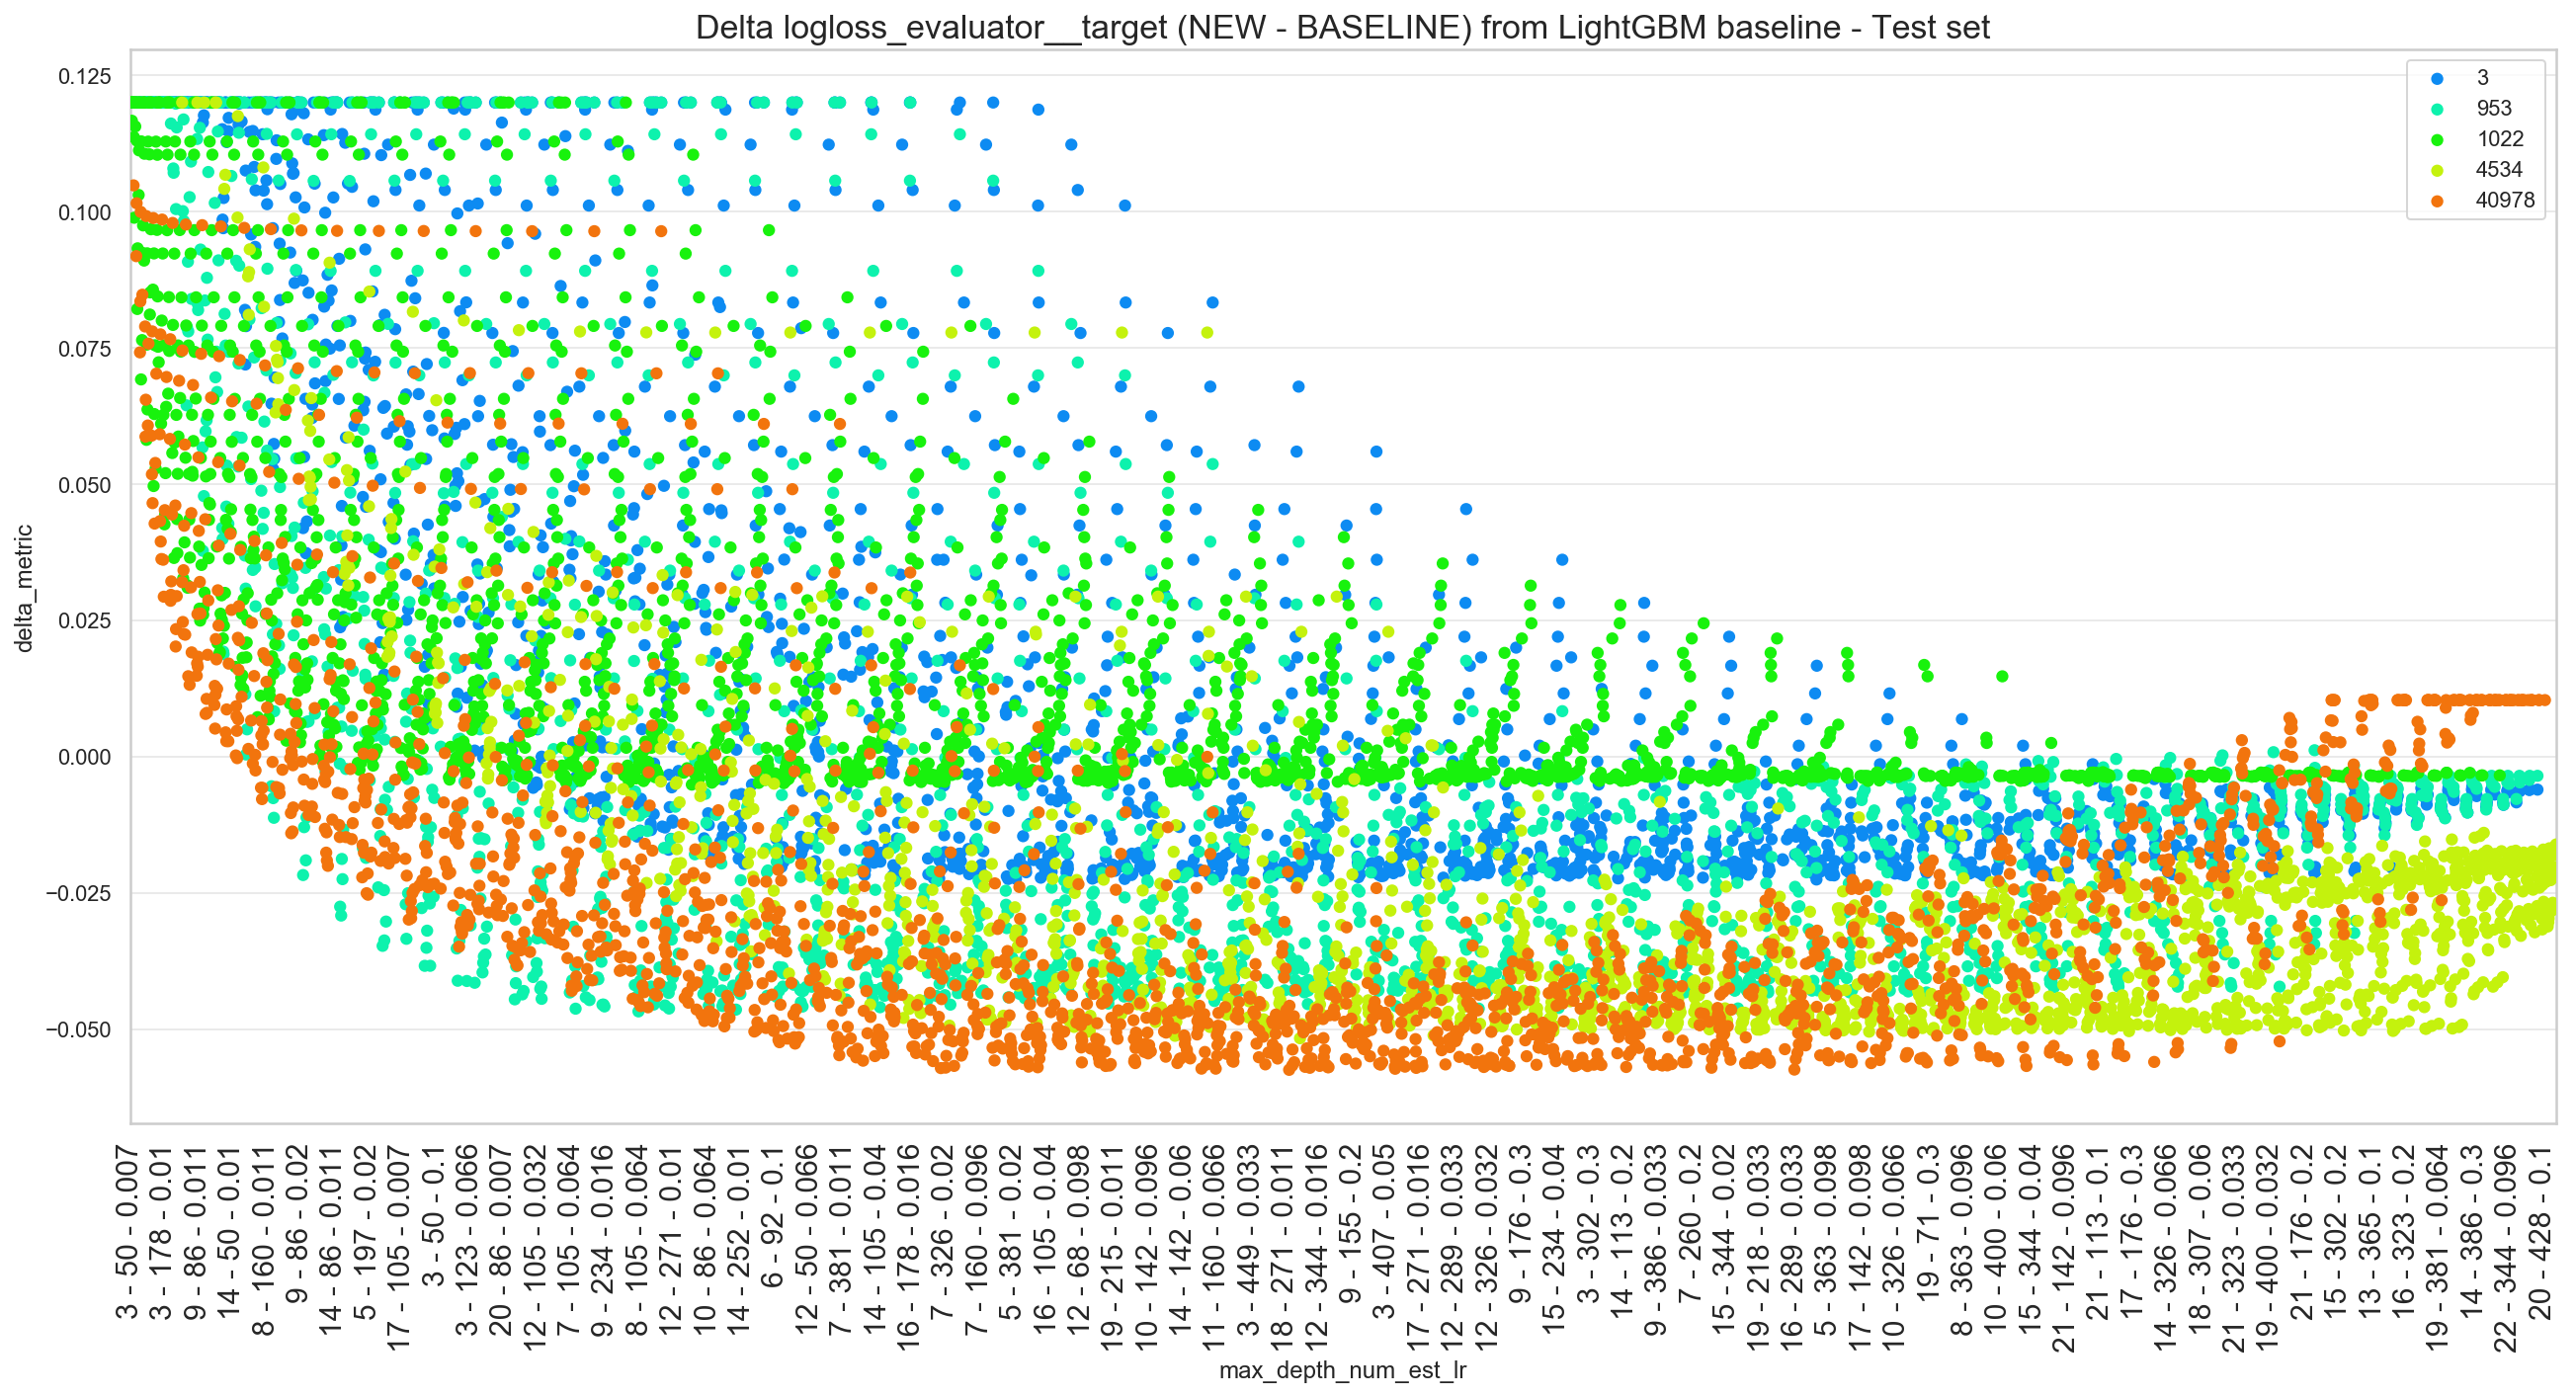
\includegraphics[width=.9\textwidth]{delta_logloss-cluster3-nemdlr.png}
    \caption{$\delta_{Logloss}$ for scenario $\mathcal{S}(C_2, \eta^{(2)}_{NE, MD, LR}, Logloss)$}
    \label{fig:delta-nemdlr-1}
\end{figure}

\begin{figure}[H]
    \centering
    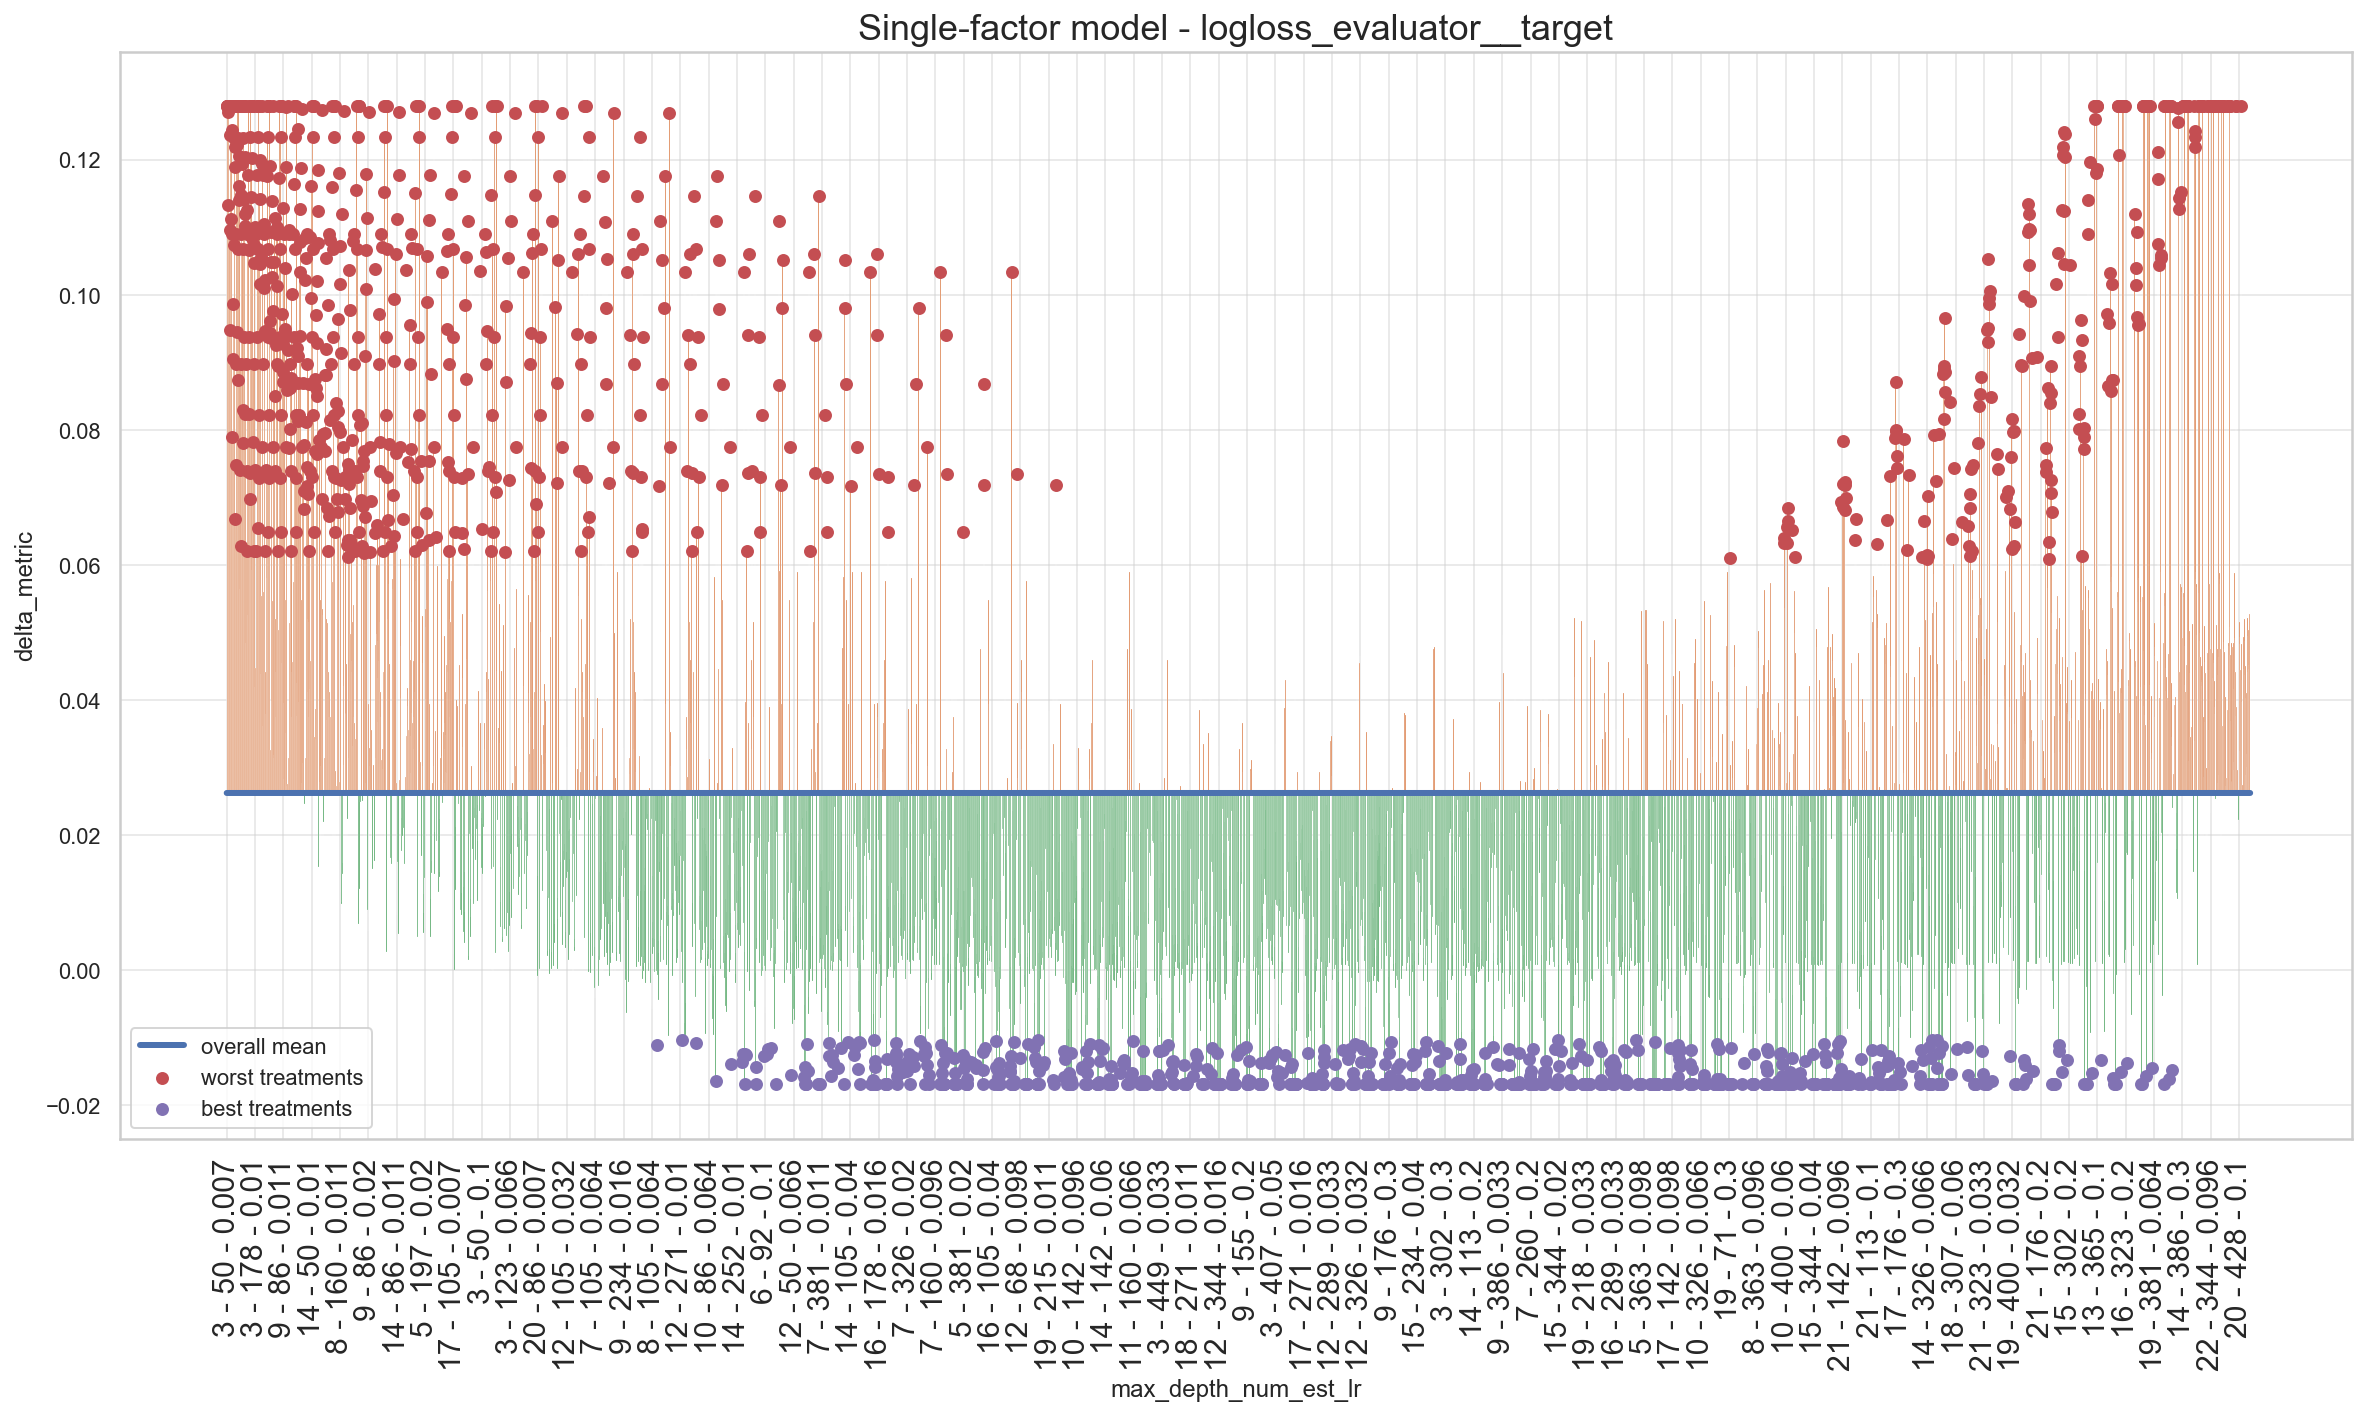
\includegraphics[width=.9\textwidth]{sfm-cluster3-logloss-nemdlr.png}
    \caption{SFM plot for $\mathcal{S}(C_2, \eta^{(2)}_{NE, MD, LR}, Logloss)$}
    \label{fig:sfm-nemdlr-1}
\end{figure}

In some metrics and clusters, the SFM plot for $\eta_{NE, MD, LR}$ is very noisy, probably due to a high dimensionality reduction in the x axis, which makes it even more difficult to interpret it, as illustrated in Figure \ref{fig:sfm-nemdlr-2}. Overall, 

\begin{figure}[H]
    \centering
    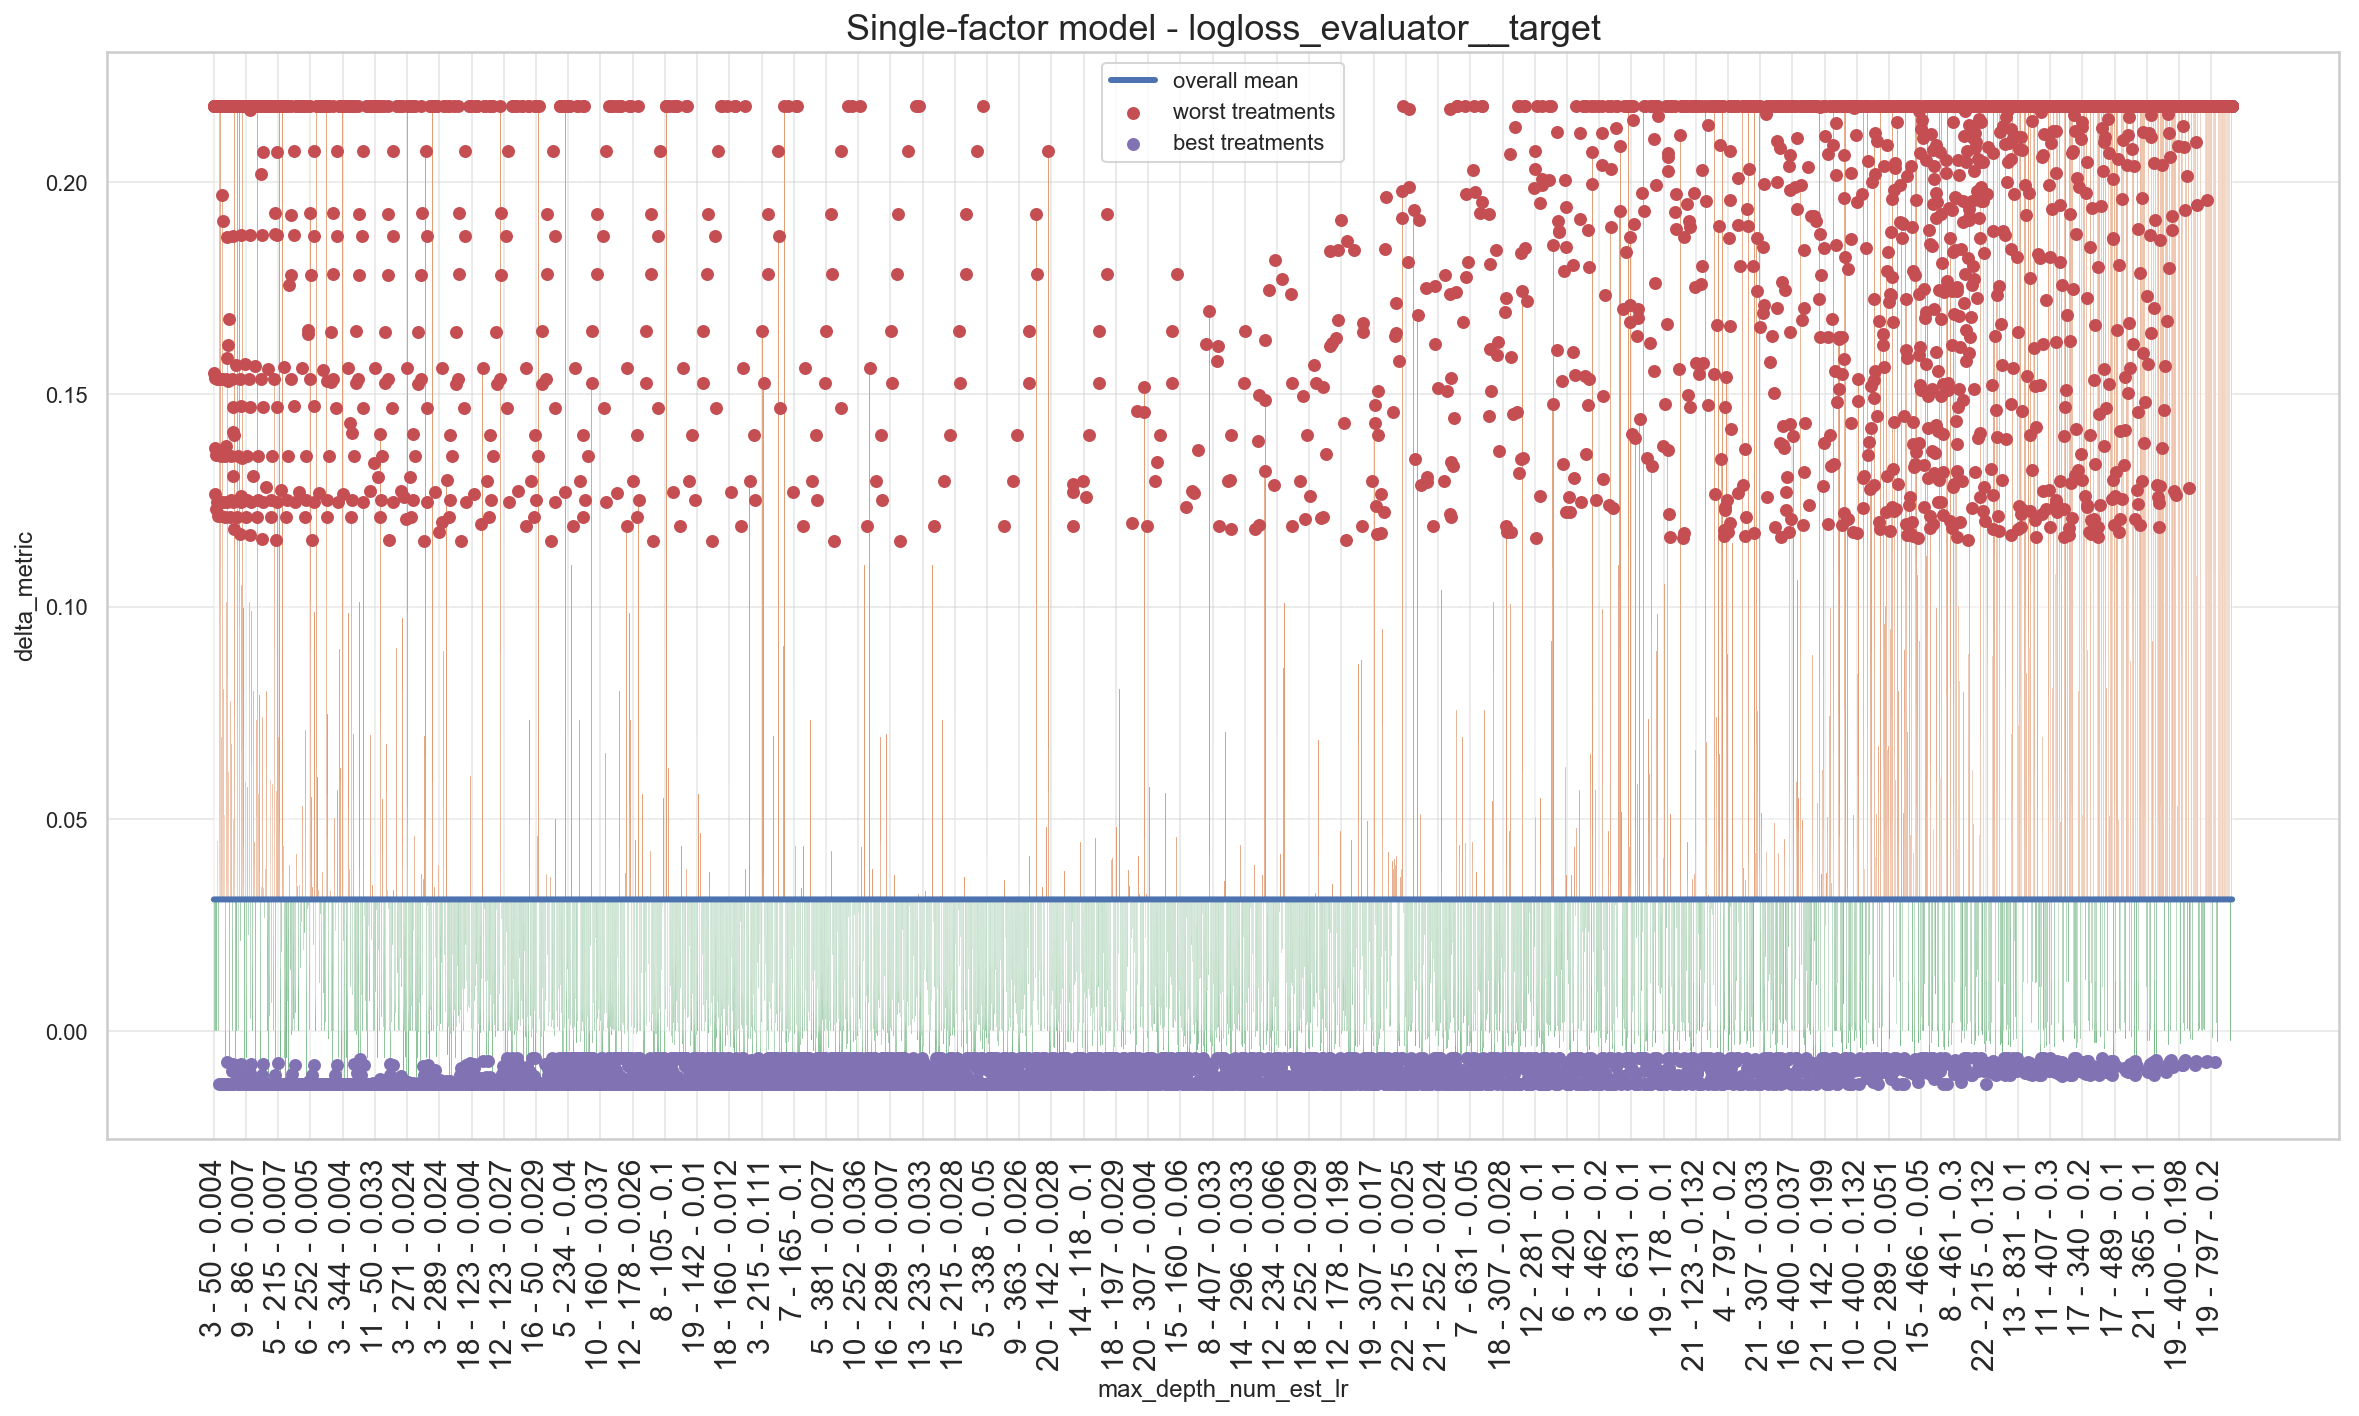
\includegraphics[width=.9\textwidth]{sfm-cluster1-logloss-nemdlr.png}
    \caption{SFM plot for $\mathcal{S}(C_1, \eta^{(1)}_{NE, MD, LR}, Logloss)$}
    \label{fig:sfm-nemdlr-2}
\end{figure}

%% ------------------------------------------------------------------------- %%
\section{Results by Hyperparameter Combination Effect}

Another perspective of analysis of the experiments results is about the ``combination effect'' of the hyperparameters, i.e. how changing one hyperparameter individually, in pairs or in triples differ in terms of significant difference in the performance metrics $\delta_{metric}$.

Theoretically, training models while changing multiple hyperparameters in a model tuning process means more hyperparameter space is covered. For example, the Random Search algorithm (see \cite{probst2018tunability}) typically change more than one hyperparameter value at a time, searching for a more ``extensive'' hyperparameter space than changing just a single hyperparameter value each time. This fact can be confirmed in study, at least for the clusters analyzed here. Table \ref{table:stats-combination} show the percentage of scenarios which a significant change in the metrics was observed in the study.

\begin{table}[H]
    \centering
    \begin{tabular}{l|lcc}
              & \multicolumn{3}{c}{\textbf{Metric}}                                 \\
              & \multicolumn{1}{c}{$\delta_{AUC}$} &  \multicolumn{1}{c}{$\delta_{Brier}$} &  \multicolumn{1}{c}{$\delta_{Logloss}$} \\
    \textbf{Combinations} &          & \multicolumn{1}{l}{} & \multicolumn{1}{l}{} \\
    \midrule
    Individual & $22.2\%$ & $22.2\%$ & $38.8\%$\\
    Pair       & $38.8\%$ & $55.5\%$ & $50\%$\\
    Triple     & $66.6\%$ & $66.6\%$ & $66.6\%$
    \end{tabular}
    \caption{Percentage of statistically significant results for each comparison and metric}
    \label{table:stats-combination}
\end{table}

In practice changing several hyperparameters at the same time can be costly, which is one of the reasons a Bayesian Optimization or multi-stage optimization can be performed, e.g. the multi-stage algorithm described in \cite{wang-etal-2015-efficient}. Using the results of this study, the typical trade-off between computational complexity and search space in the model tuning can be better evaluated depending on the case. For instance, one could start a gradient boosting model tuning process by changing \code{max\_depth} and \code{learning\_rate} at the same time, as it is a pair of hyperparameters (it is faster to run than a triple or higher number of combinations) that resulted in a high percentage of statistically significant SFM models (the models are highly sensitive to this combination of hyperparameters).

    
%% ------------------------------------------------------------------------- %%
\section{Results by Cluster}

Each cluster result can also provide useful insights related to the datasets inside the cluster and how sensitive they are w.r.t different combinations of hyperparameters. In this section the main observations from each cluster results are addressed, along with possible explanations for their behavior.

By using table \ref{table:stats-sig} from Section \ref{sec:stats-significance}, it is possible to summarize the results of the experiments grouping by the cluster number. Table \ref{table:stats-clusters} describes the proportion of statistically significant experiments for each metric on each cluster. This table gives an idea of how sensitive each cluster is to changes in the performance metrics, when subjected to all treatments of this study.

\begin{table}[H]
    \centering
    \begin{tabular}{l|cccccc}
              & \multicolumn{6}{c}{\textbf{\large Cluster}}                                    \\
              & \textbf{1} & \textbf{2} & \textbf{3} & \textbf{4} & \textbf{5} & \textbf{6}    \\
    \textbf{\large Metric} &          &          &          &          &          &          \\
    \midrule
    $\delta_{AUC}$         & $42.8\%$ & $57.1\%$ & $28.5\%$ & $0.0\%$  & $57.1\%$ & $42.8\%$ \\
    $\delta_{Brier}$       & $57.1\%$ & $57.1\%$ & $14.2\%$ & $42.8\%$ & $71.4\%$ & $14.2\%$ \\
    $\delta_{Logloss}$     & $71.4\%$ & $85.7\%$ & $0.0\%$  & $42.8\%$ & $71.4\%$ & $14.2\%$ \\
    \midrule
                   Overall & $57.1\%$ & $66.6\%$ & $14.2\%$ & $28.5\%$ & $66.6\%$ & $23.8\%$ 
    \end{tabular}
    \caption{Percentage of statistically significant results in each cluster, by metric}
    \label{table:stats-clusters}
\end{table}

The most \textbf{insensitive cluster}, i.e. the cluster with the least number of statistically significant experiments is \textbf{Cluster 3}. As said in Subsection \ref{subsec:clustering-strat}, all the datasets of this cluster are synthetically generated datasets, and all of them have $\geq 100000$ rows in them.  However, when looking at the statistical test results of Cluster 3, it is  the cluster which rejected the most the null hypothesis of equal variance, i.e. it is the most heteroscedastic cluster. With further analysis, some of its datasets also have a very constant $\delta_{metric}$ in the metrics, another evidence or the insensitivity of this cluster: in Figure \ref{fig:delta-auc-cluster3-mdne} the $\delta_{AUC}$ for scenario $\mathcal{S}(C_3, \eta^{(3)}_{MD, NE}, AUC)$ shows that most of the datasets have a constant $\delta_{AUC}$ regardless of the changes in maximum depth and number of estimators.

\begin{figure}[H]
    \centering
    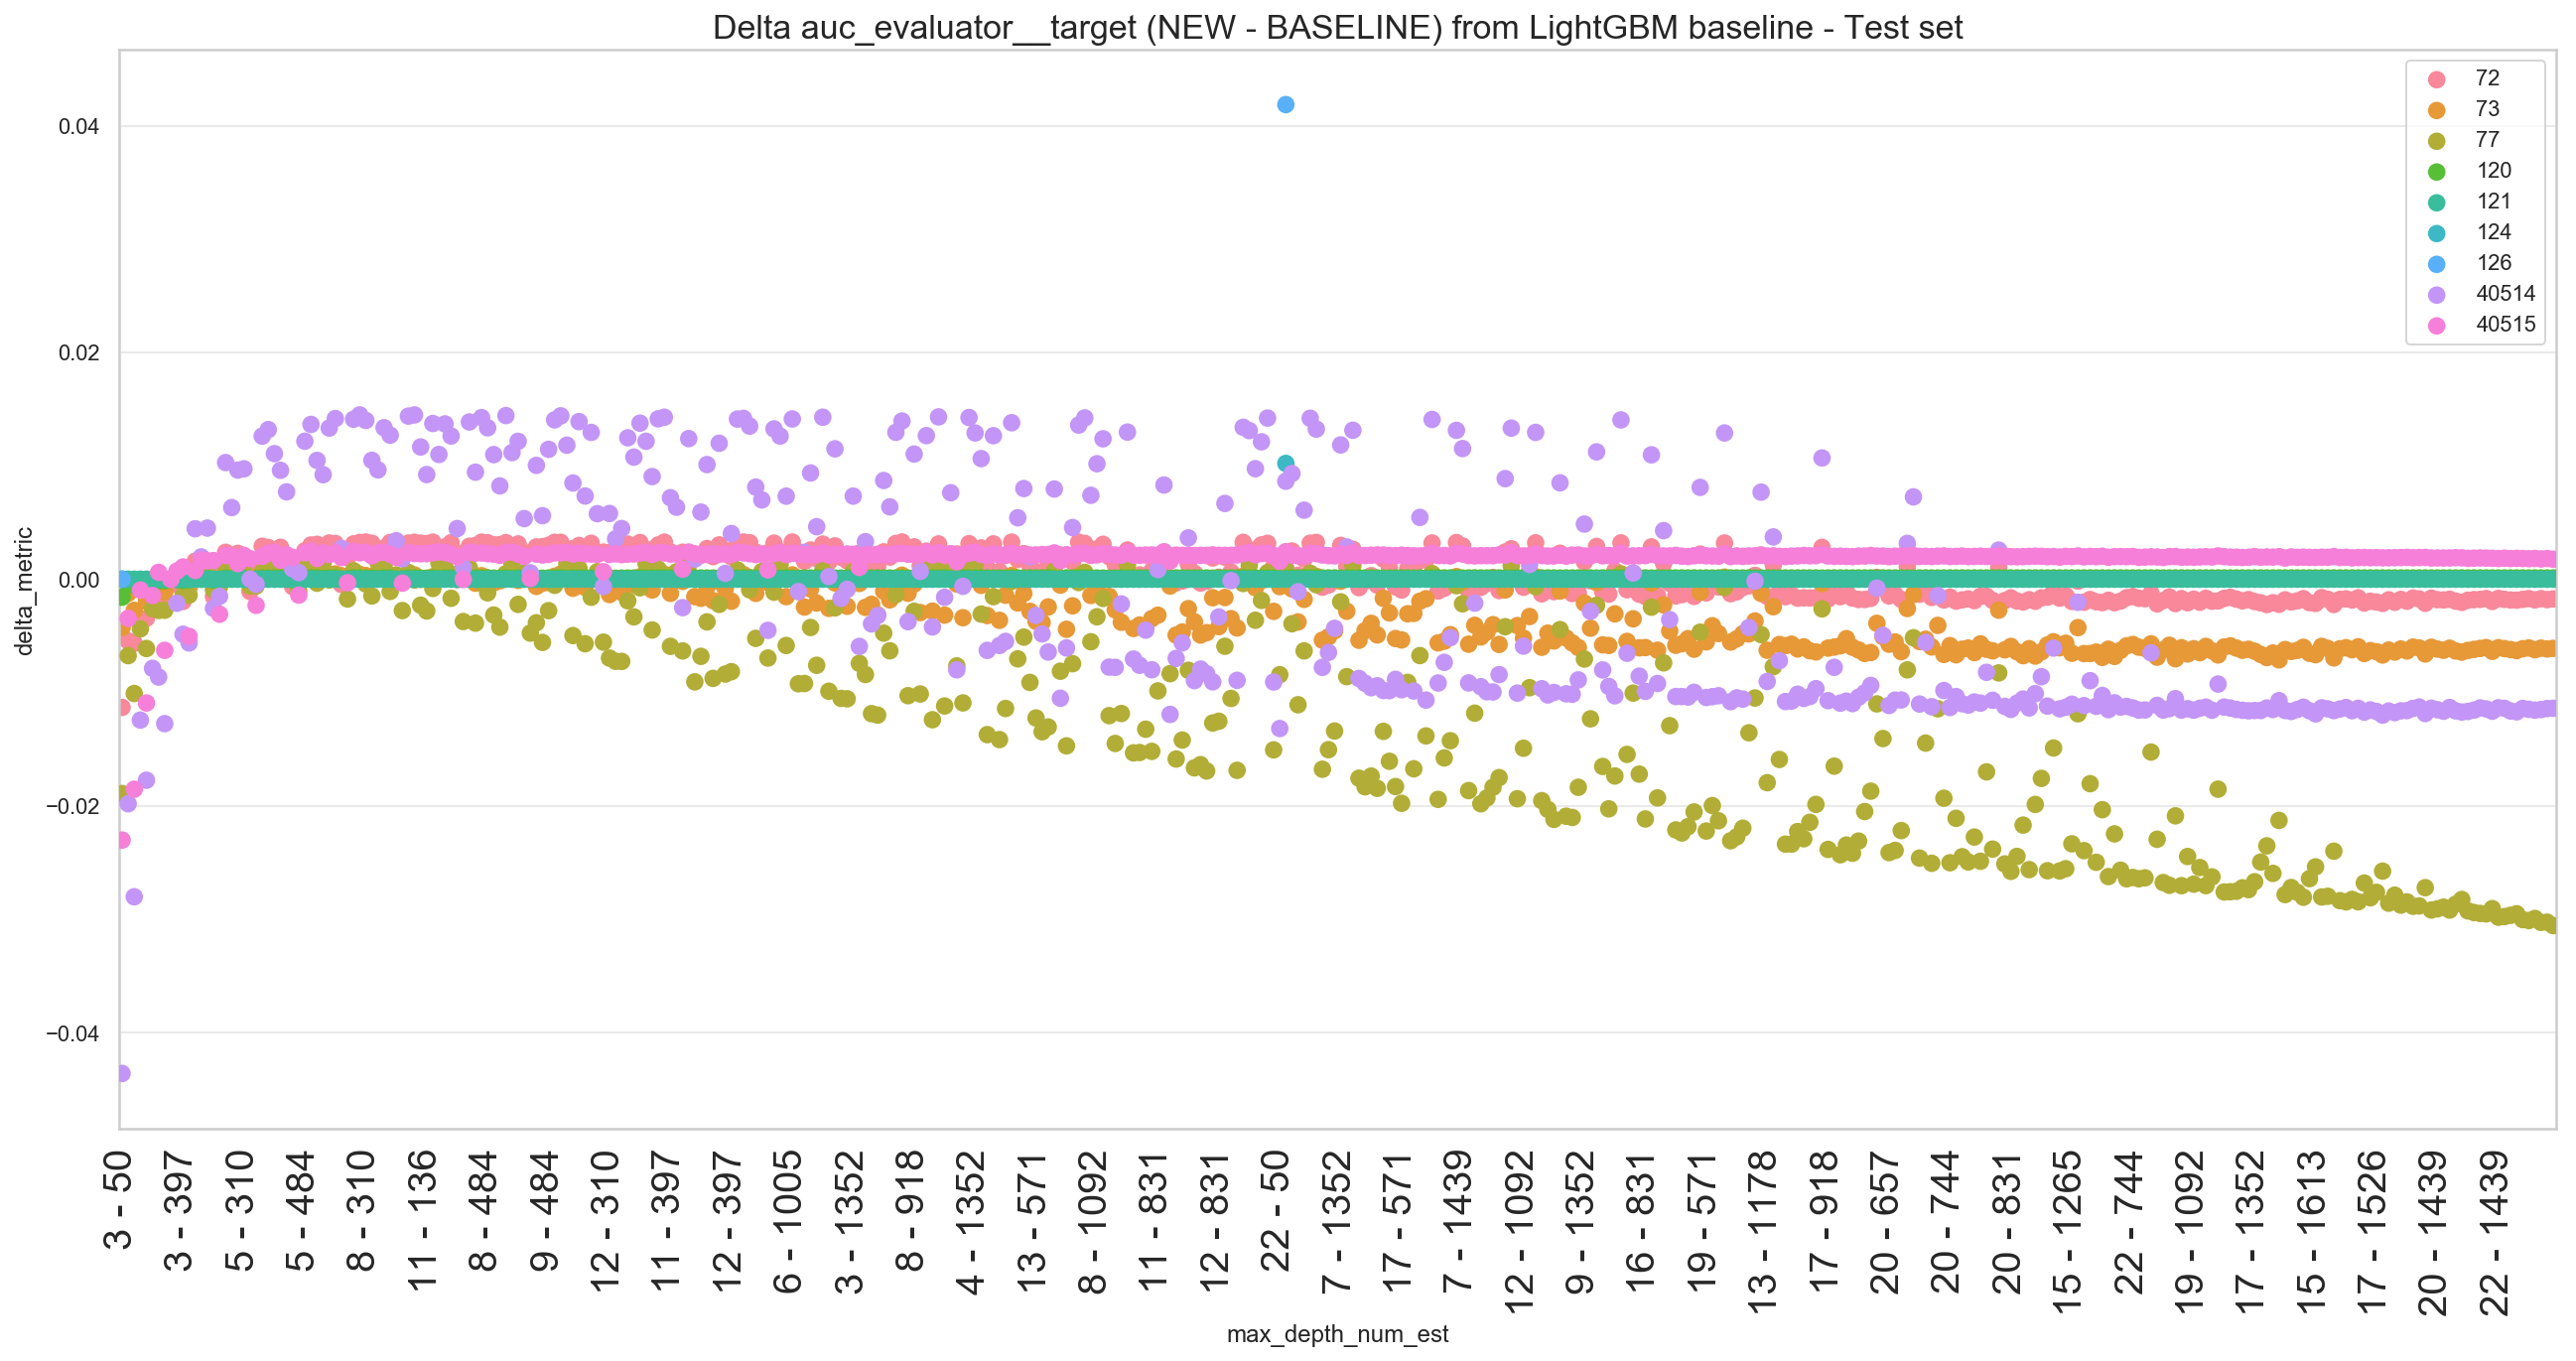
\includegraphics[width=.9\textwidth]{delta-auc-cluster3-mdne.png}
    \caption{$\delta_{AUC}$ plot for $\mathcal{S}(C_3, \eta^{(3)}_{MD, NE}, AUC)$ - only two datasets seem to change the AUC}
    \label{fig:delta-auc-cluster3-mdne}
\end{figure}

On the other hand, the most \textbf{sensitive clusters} are \textbf{Cluster 2} and \textbf{Cluster 5}. Analyzing the datasets aggregated characteristics (more details about them in Subsection \ref{subsec:agg-characteristics}) of both clusters, they are fairly similar: both have almost no numerical features, with a high proportion of categorical features; the number of rows is also similar, but Cluster 2 datasets typically have more rows than Cluster 5. The main difference between them is the number of features, where Cluster 2 datasets can have from 2 to 200 features and Cluster 5 datasets typically range from 10 to 20.

In Figure \ref{fig:sfm-cluster2-cluster5} two SFM plots of statistically significant experiments showcase both the behavior of max depth explained in Subsection \ref{subsec:analysis-md}, and also the impact of the number of features in max depth performance. One can see that the amount of tree depth needed to capture more information --- reflected here as a lower Brier Score --- is smaller when the datasets have less features. In Figure \ref{fig:sfm-c2c5-c5} max depth of $6$ is enough to have a negative treatment effect (in this case, an improvement over the baseline Brier Score), while for Cluster 2 which has more features this value is $9$, as illustrated in Figure \ref{fig:sfm-c2c5-c2}.


\begin{figure}[!h]
    \centering
    \begin{subfigure}[b]{0.49\textwidth}
        \centering
        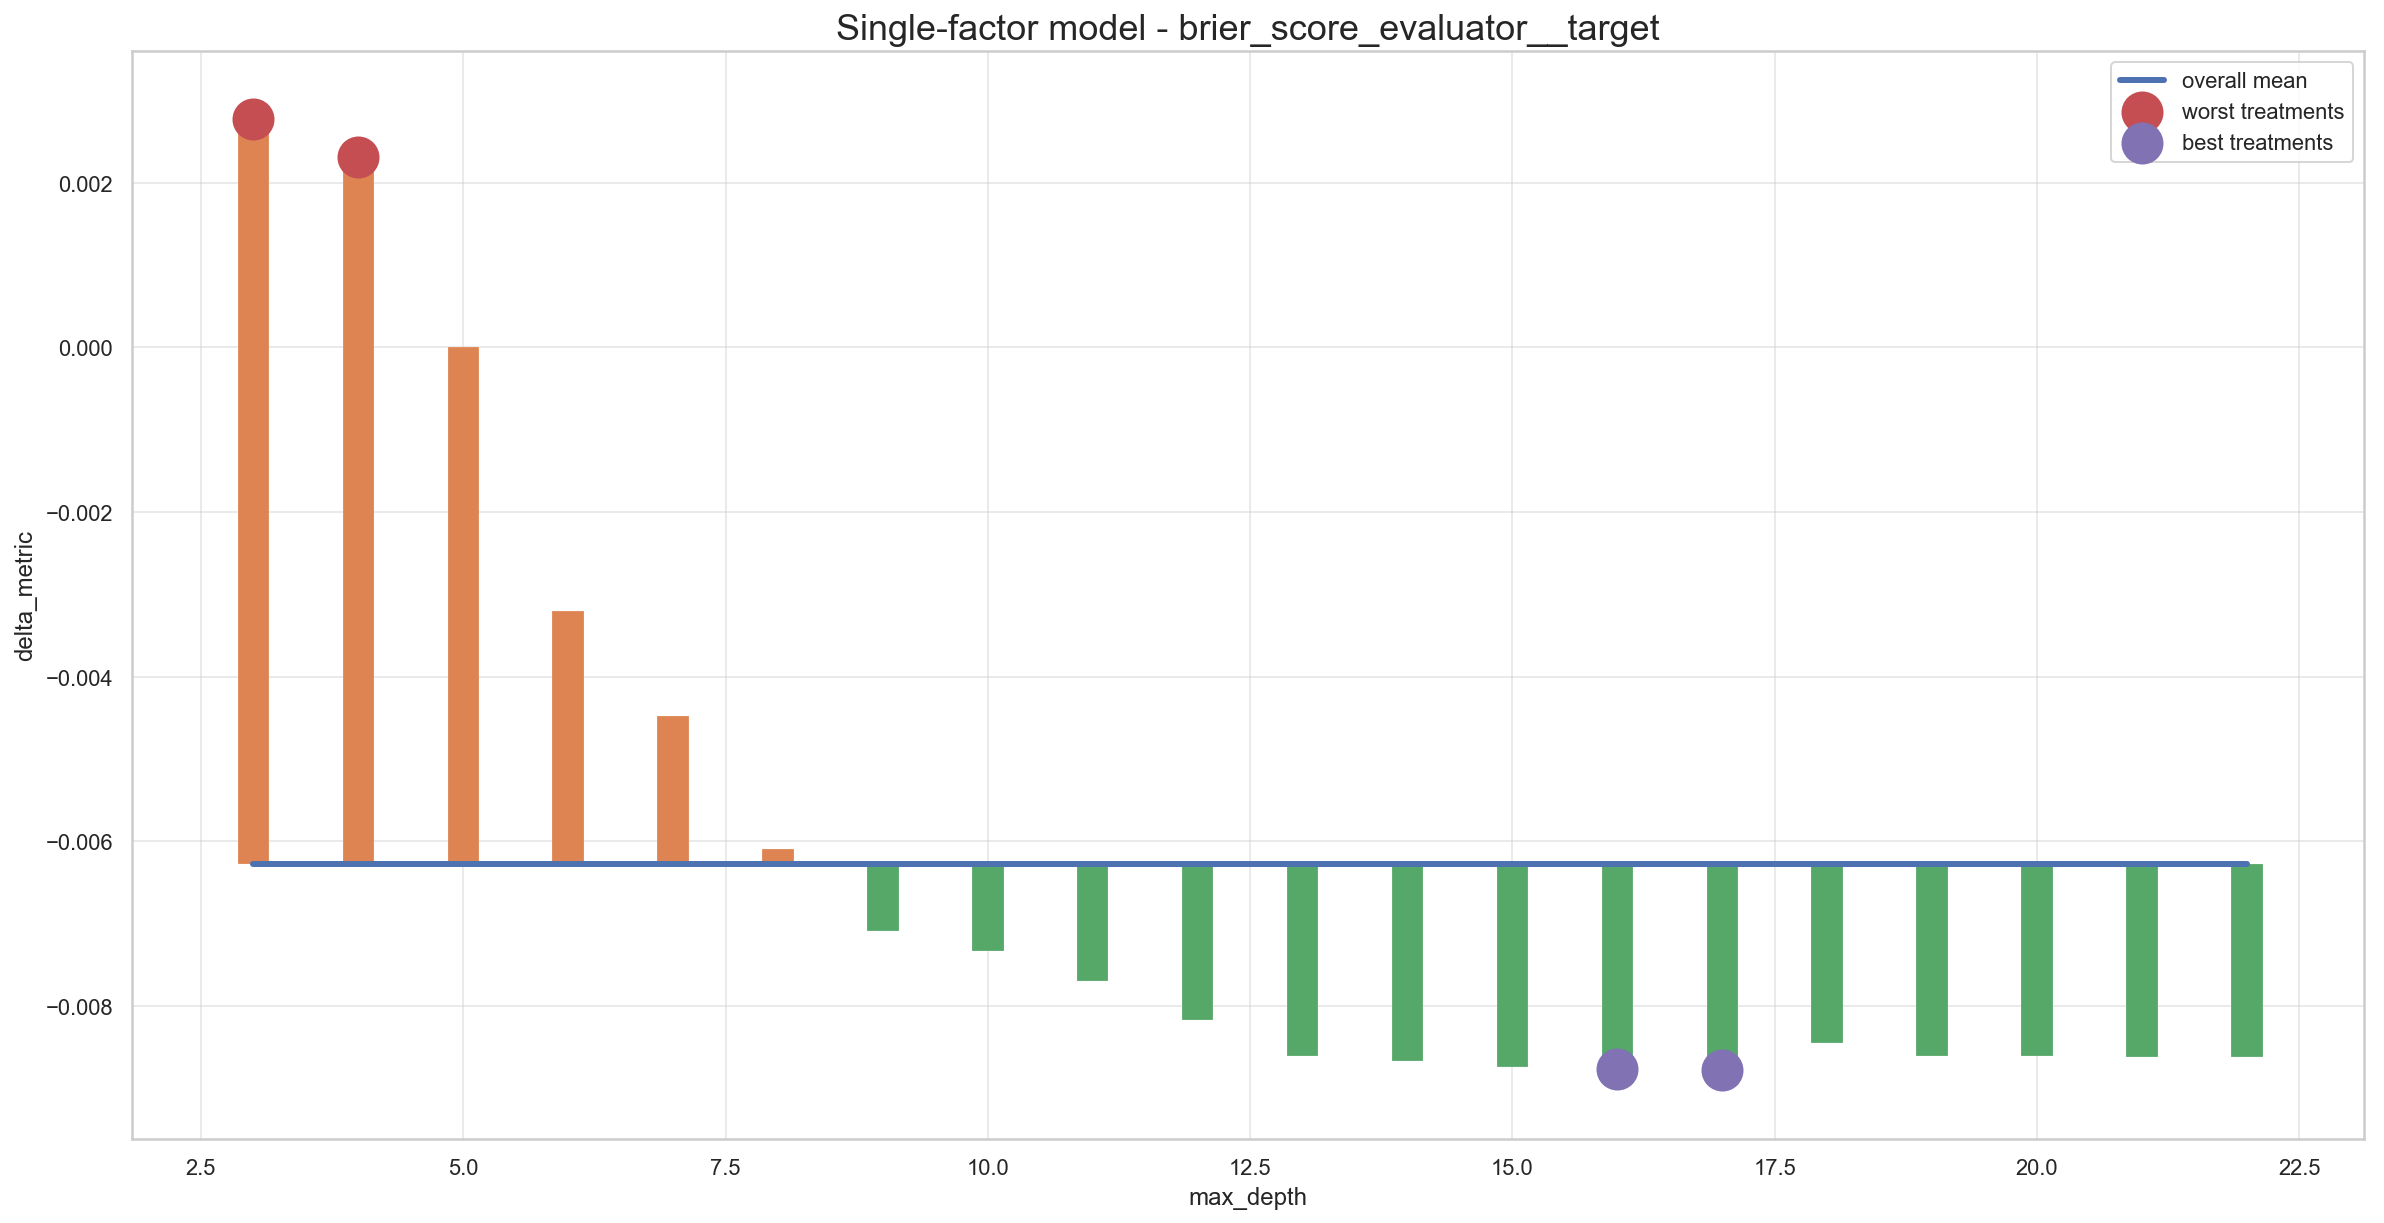
\includegraphics[width=\textwidth]{sfm-cluster2-brier-md.png}
        \caption{$\mathcal{S}(C_2, \eta^{(2)}_{MD}, Brier)$}
        \label{fig:sfm-c2c5-c2}
    \end{subfigure}
    \hfill
    \begin{subfigure}[b]{0.49\textwidth}
        \centering
        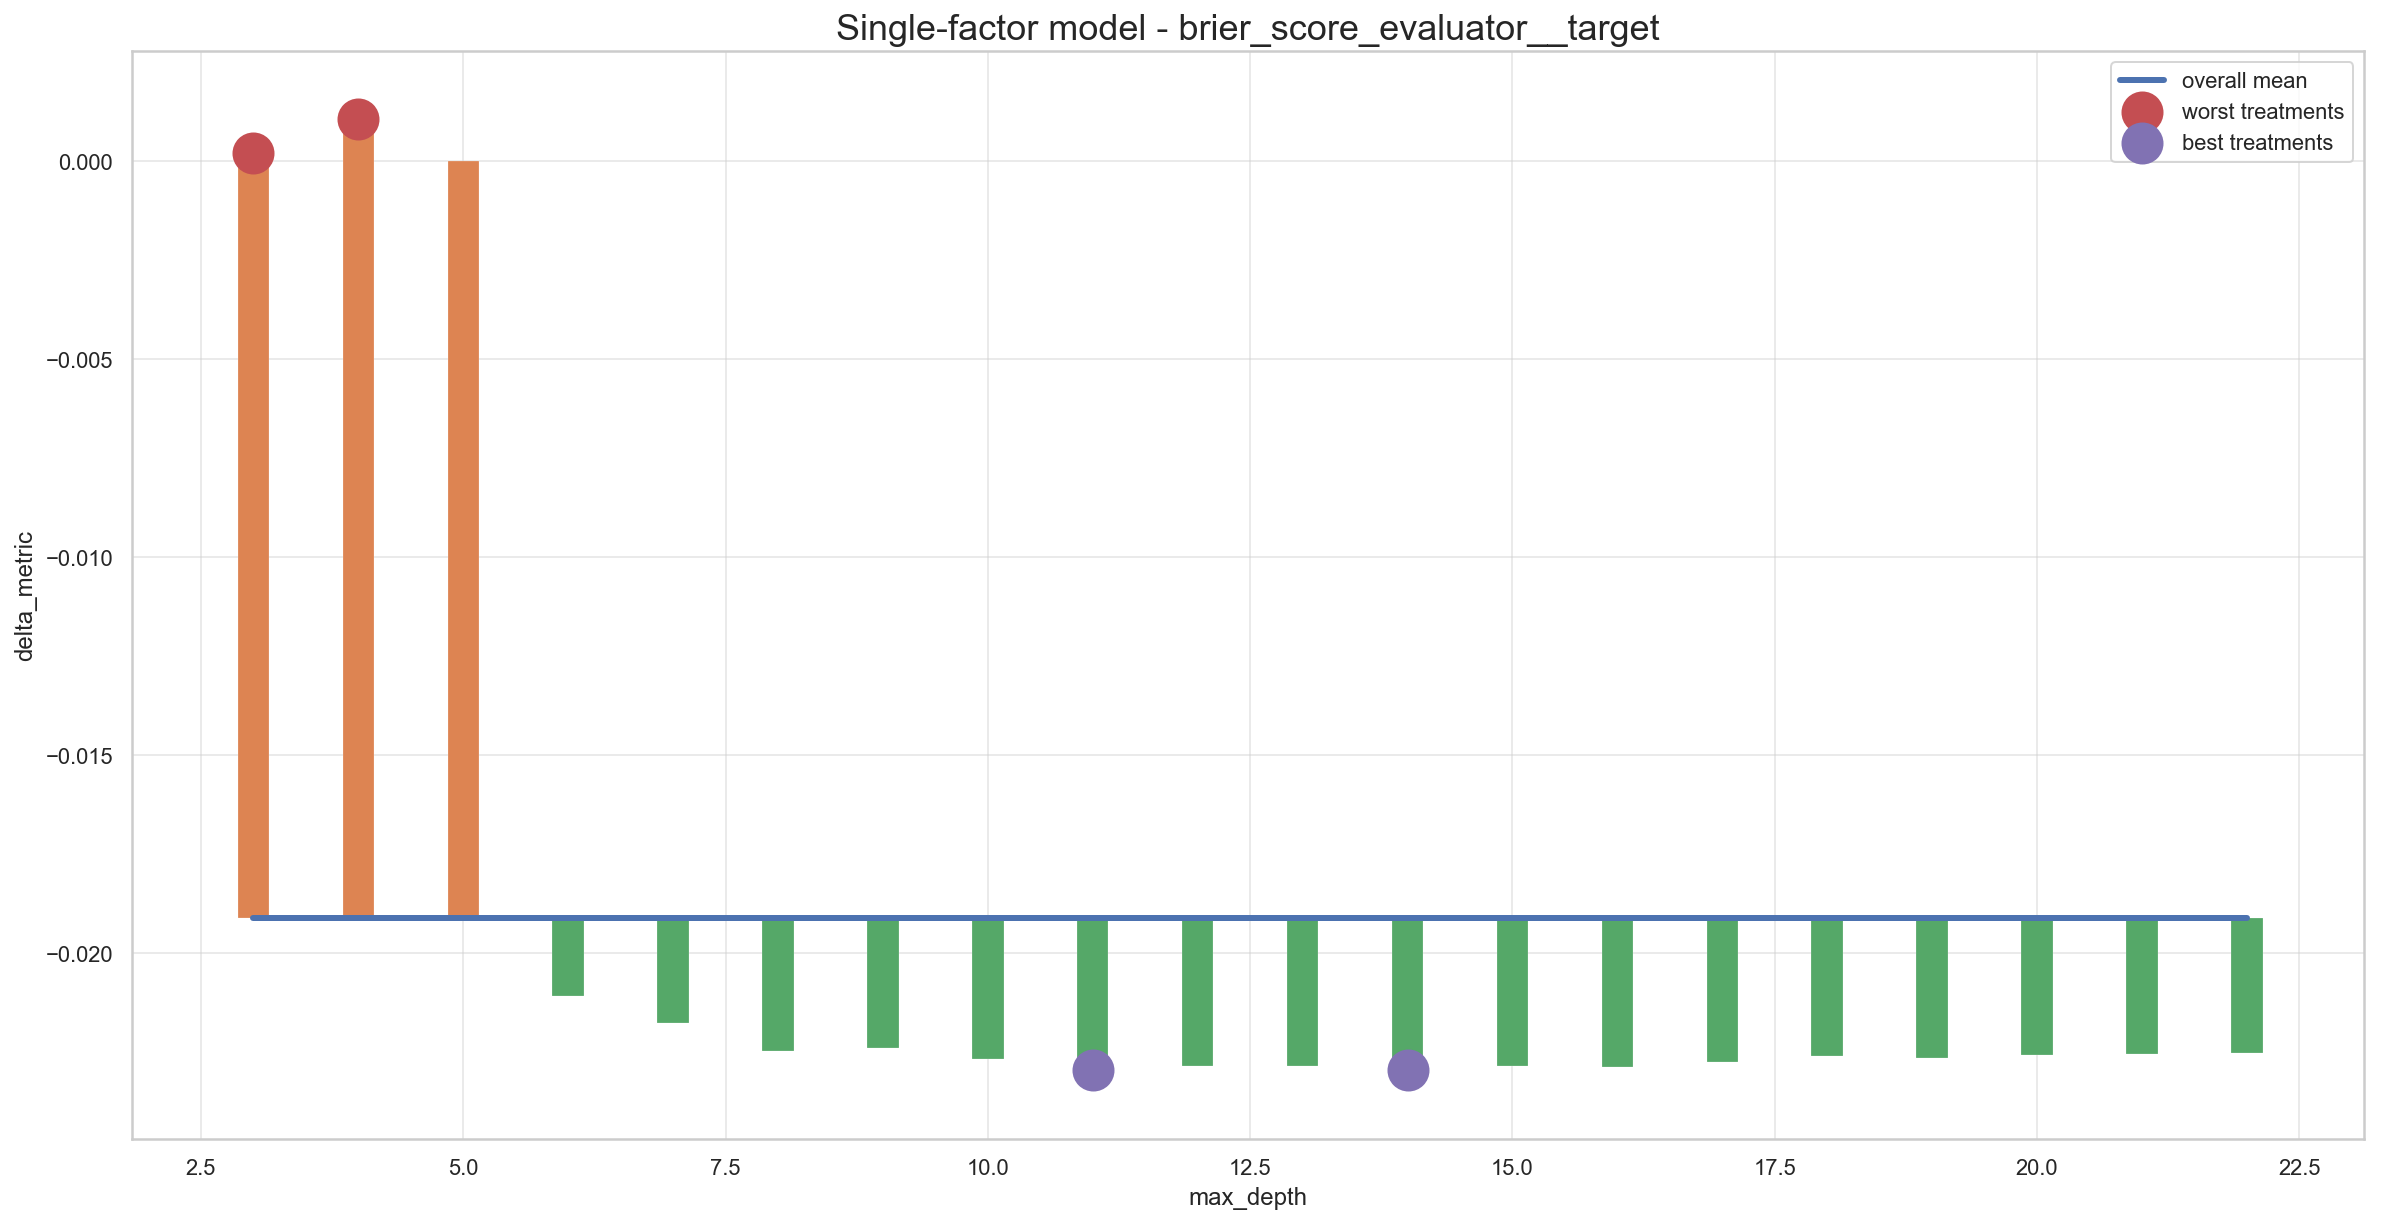
\includegraphics[width=\textwidth]{sfm-cluster5-brier-md.png}
        \caption{$\mathcal{S}(C_5, \eta^{(5)}_{MD}, Brier)$}
        \label{fig:sfm-c2c5-c5}
    \end{subfigure}
    \hfill
       \caption{Two SFM plots of $\eta_{MD}$ and $\delta_{Brier}$ on Cluster 2 and 5, respectively}
       \label{fig:sfm-cluster2-cluster5}
\end{figure}


Finally, it is interesting to note that Cluster 4 does not have a single statistically significant experiment when the performance metric is $\delta_{AUC}$, and when an experimental scenario with $\delta_{Brier}$ rejected the null hypothesis of equality of treatment means the corresponding scenario with $\delta_{Logloss}$ also rejected it, and vice versa.

%% ------------------------------------------------------------------------- %%
\section{Results by Metrics}

Regarding the performance metrics of the study, described in  Section \ref{classification-metrics}, there are some insights about their results from the experimental scenarios. Table \ref{table:stats-metrics} illustrates the proportion of scenarios with significant change in the $\delta_{metric}$: The Logloss metric is the most sensitive in this study, changing in almost 50\% of the experiments. It is closely followed by the Brier Score, and the least sensitive metric in the study is the AUC.

\begin{table}[H]
    \centering
    \begin{tabular}{ccc}
              \textbf{$\delta_{AUC}$} & \textbf{$\delta_{Brier}$} & \textbf{$\delta_{Logloss}$} \\
              \midrule
              $38.1\%$&$42.7\%$&$47.6\%$
    \end{tabular}
    \caption{Percentage of statistically significant results of each metric}
    \label{table:stats-metrics}
\end{table}

The higher percentage of significance of the logarithmic loss is expected, since it is the metric being optimized in all LightGBM binary classification models of the study. Logloss is not bound to the $\left[0, 1\right]$ interval as AUC and Brier Score, which means in practice the treatment values of the Logloss aren't as interpretable when compared to other metrics. The similarity of the percentage of Table \ref{table:stats-metrics} between the Brier Score and Logloss is partially expected, as both metrics assess the value of the predicted probabilities of the classifier.

At the same time, the AUC does not directly evaluate the performance of the predicted probabilities themselves, but it actually assess the relative ordering of the classifier. For this reason, results like the one observed in Cluster 4 can happen, i.e. the relative ordering performance can be kept the same while the forecasted probabilities can be better. The highest change of the $\delta_{AUC}$ was in the experimental scenario $\mathcal{S}(C_5, \eta^{(5)}_{NE, MD, LR}, AUC)$ illustrated in Figure \ref{fig:sfm-cluster5-auc-nemdlr}, albeit mostly worse AUC than baseline --- probably because Cluster 5 datasets have relatively few instances that make the models easy to overfit.

\begin{figure}[H]
    \centering
    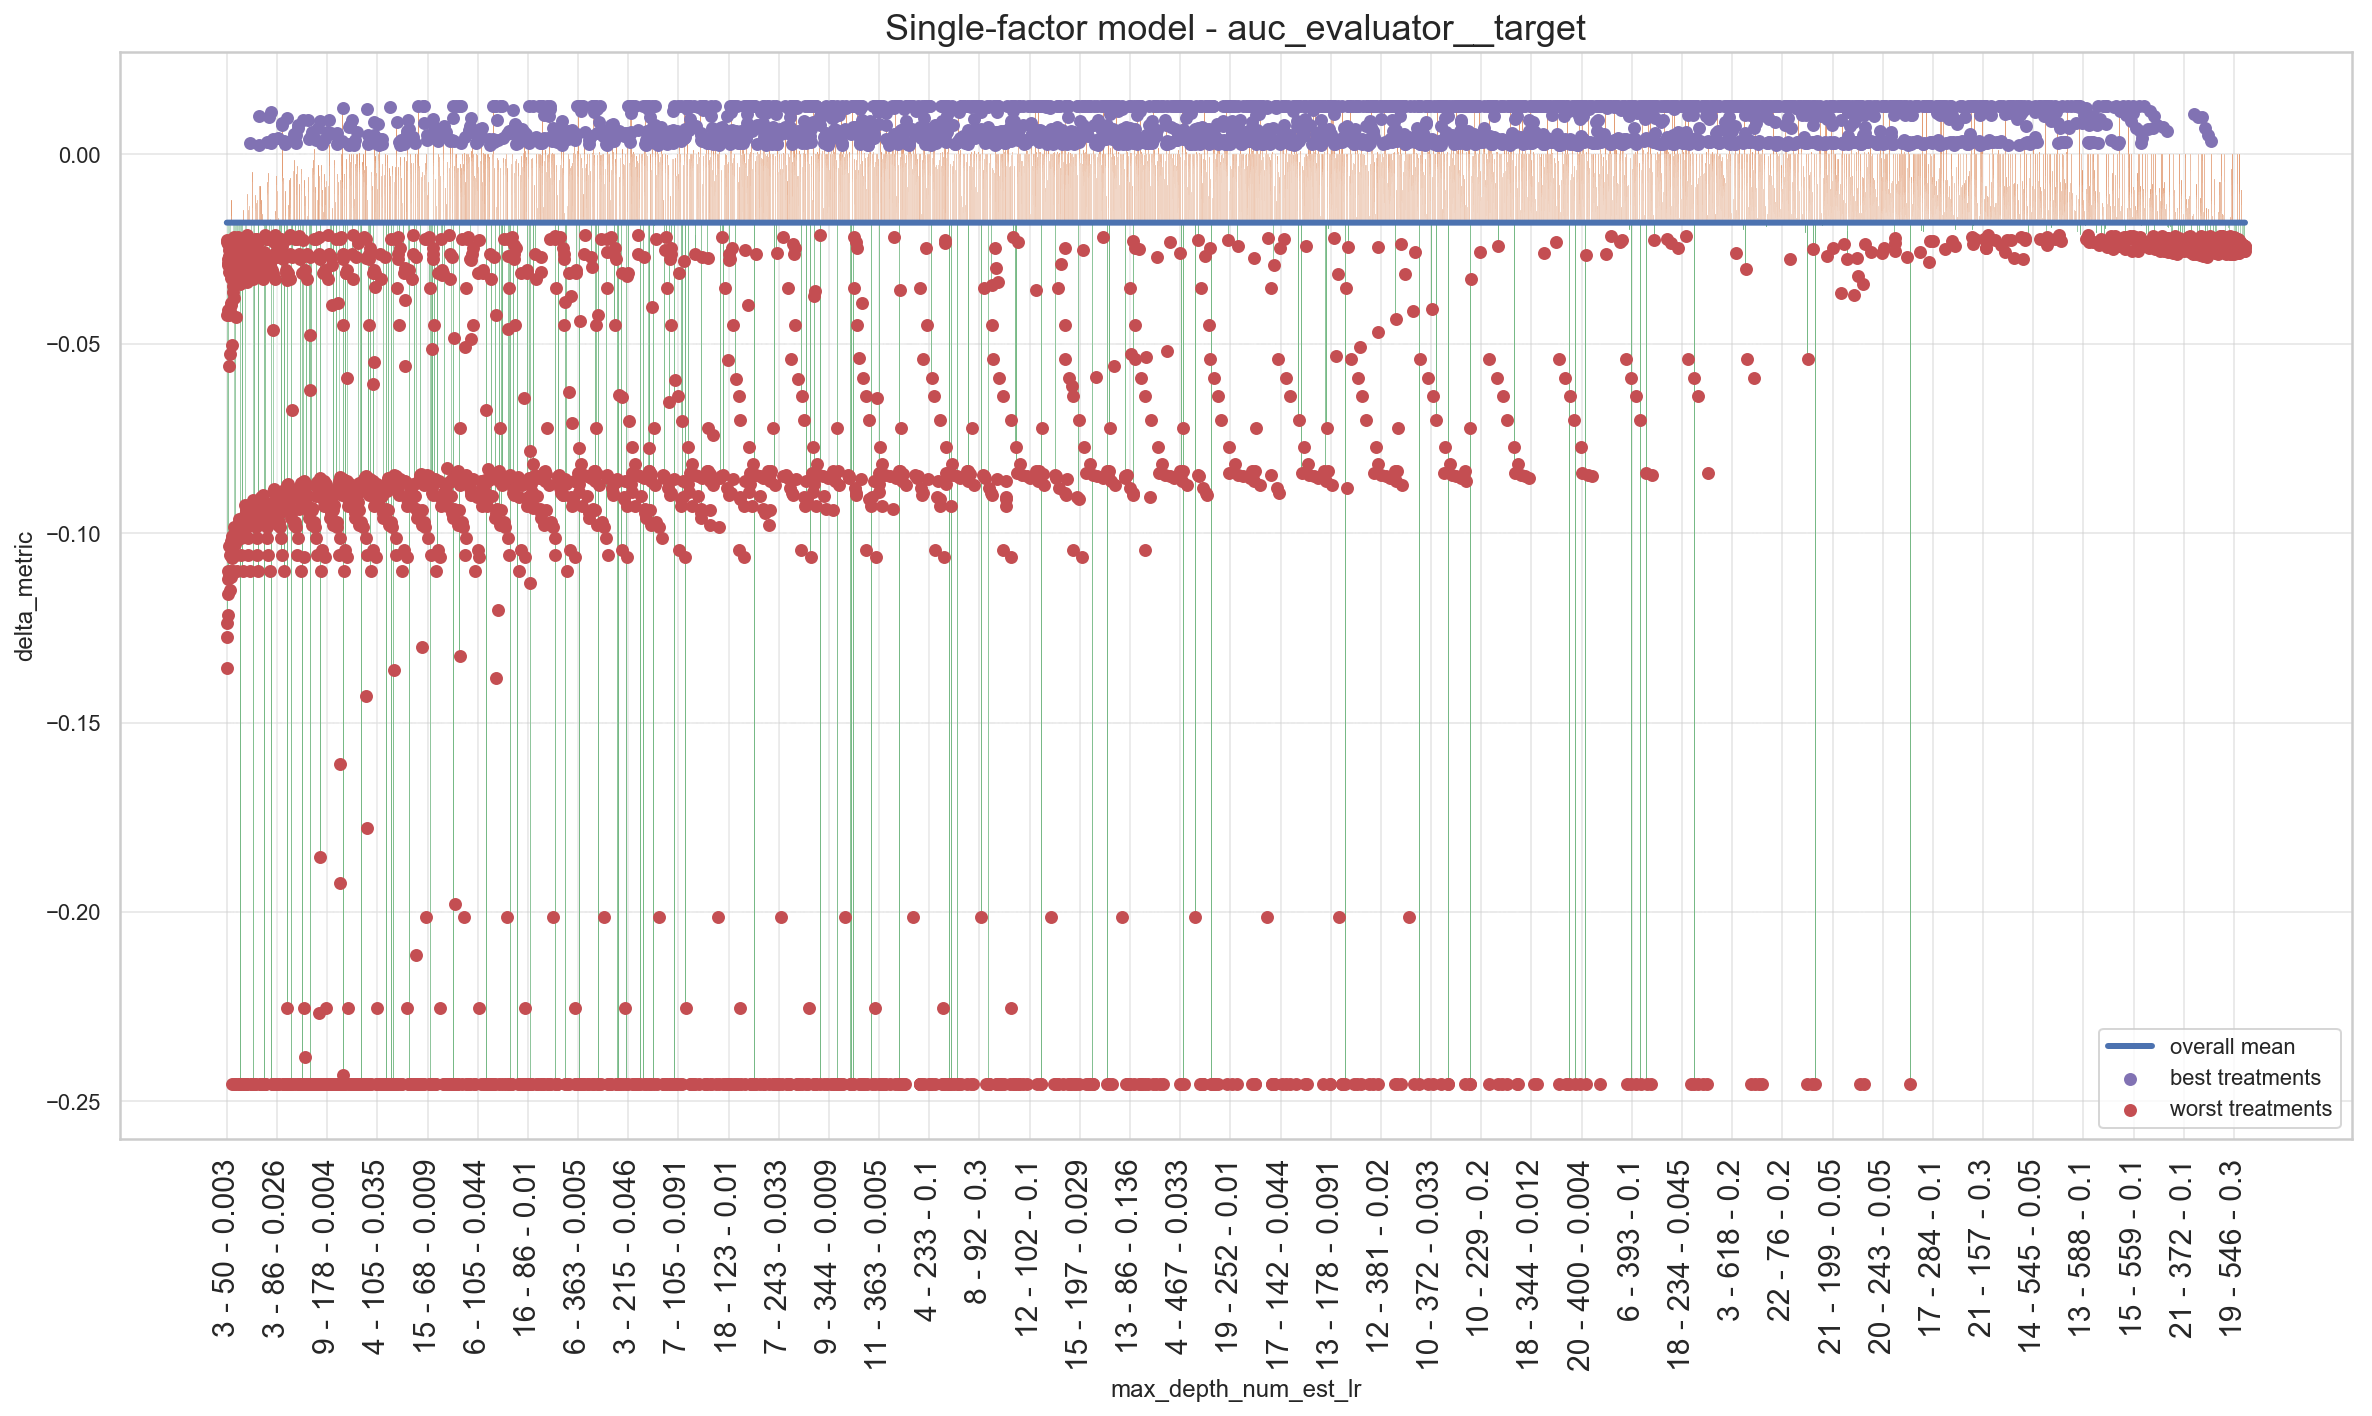
\includegraphics[width=.9\textwidth]{sfm-cluster5-auc-nemdlr.png}
    \caption{$\delta_{AUC}$ plot for $\mathcal{S}(C_5, \eta^{(5)}_{NE, MD, LR}, AUC)$}
    \label{fig:sfm-cluster5-auc-nemdlr}
\end{figure}


Several clusters in the study have imbalanced datasets, and it is known that AUC isn't the most informative metric in imbalanced situations, as described in \cite{saito2015precision}. In future work, a possible improvement is to use the Precision-Recall curve for imbalanced datasets, as it provides a better interpretation and of the classifier performance in these cases.
